%In this chapter we provide an in depth description of the various user interfaces provided by the platform.
%%TODO : use case with Philipp ?
%\section{Initial Interfaces}\label{sec:initial}
%This is the landing page of the application, where we have some information and on the top right we can see the Login and Get Started buttons, used to login and register to the platform.
%\begin{figure}[H]
%    \centering
%    
\includegraphics[width=0.8\textwidth]{Images/ui/Landing}
%    \caption{Landing Page}
%    \label{fig:landing}
%\end{figure}
%
%If we want to make an account, after pressing on the Get Started button, we are presented with the following selection.
%Here we need to specify what type of account we want to create, and we also need to agree to the terms and conditions, as well as to receiving email notifications.
%\begin{figure}[H]
%    \centering
%    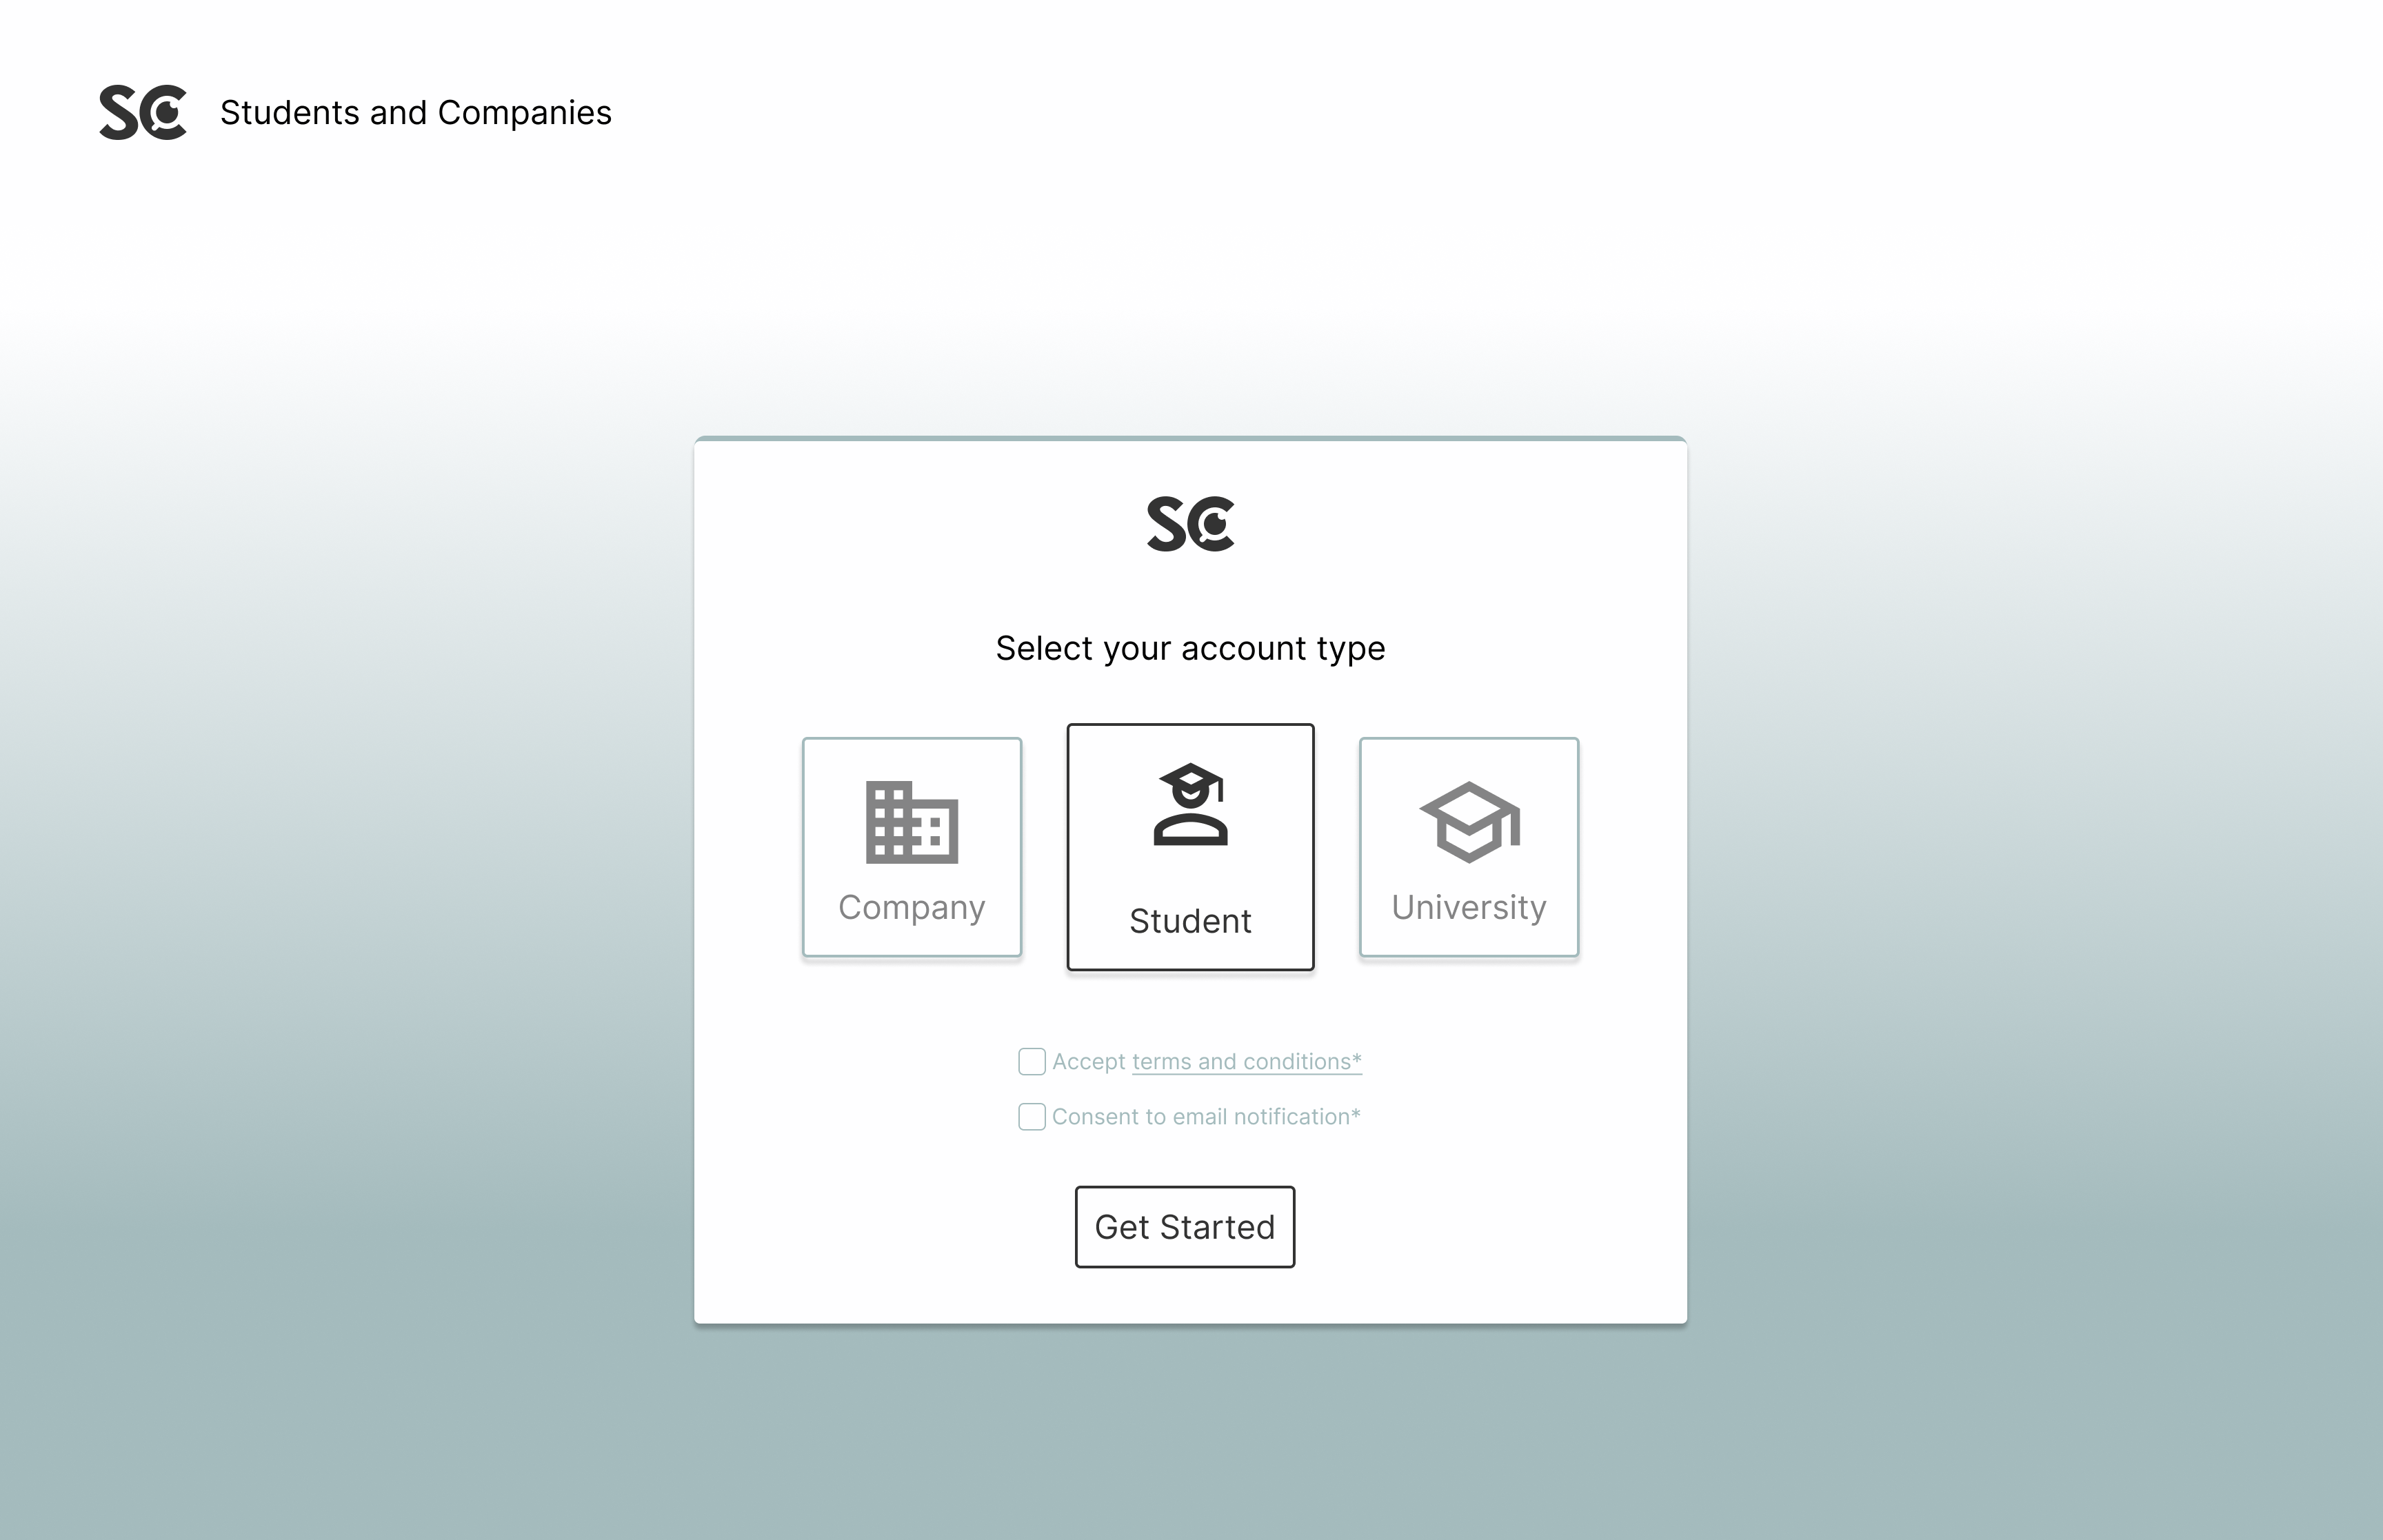
\includegraphics[width=0.8\textwidth]{Images/ui/Sign up selector}
%    \caption{SignUp Selector}
%    \label{fig:signup}
%\end{figure}
%
%Depending on which type of account we selected beforehand we are shown a different form, as we can see in the following images.
%\begin{figure}[H]
%    \centering
%    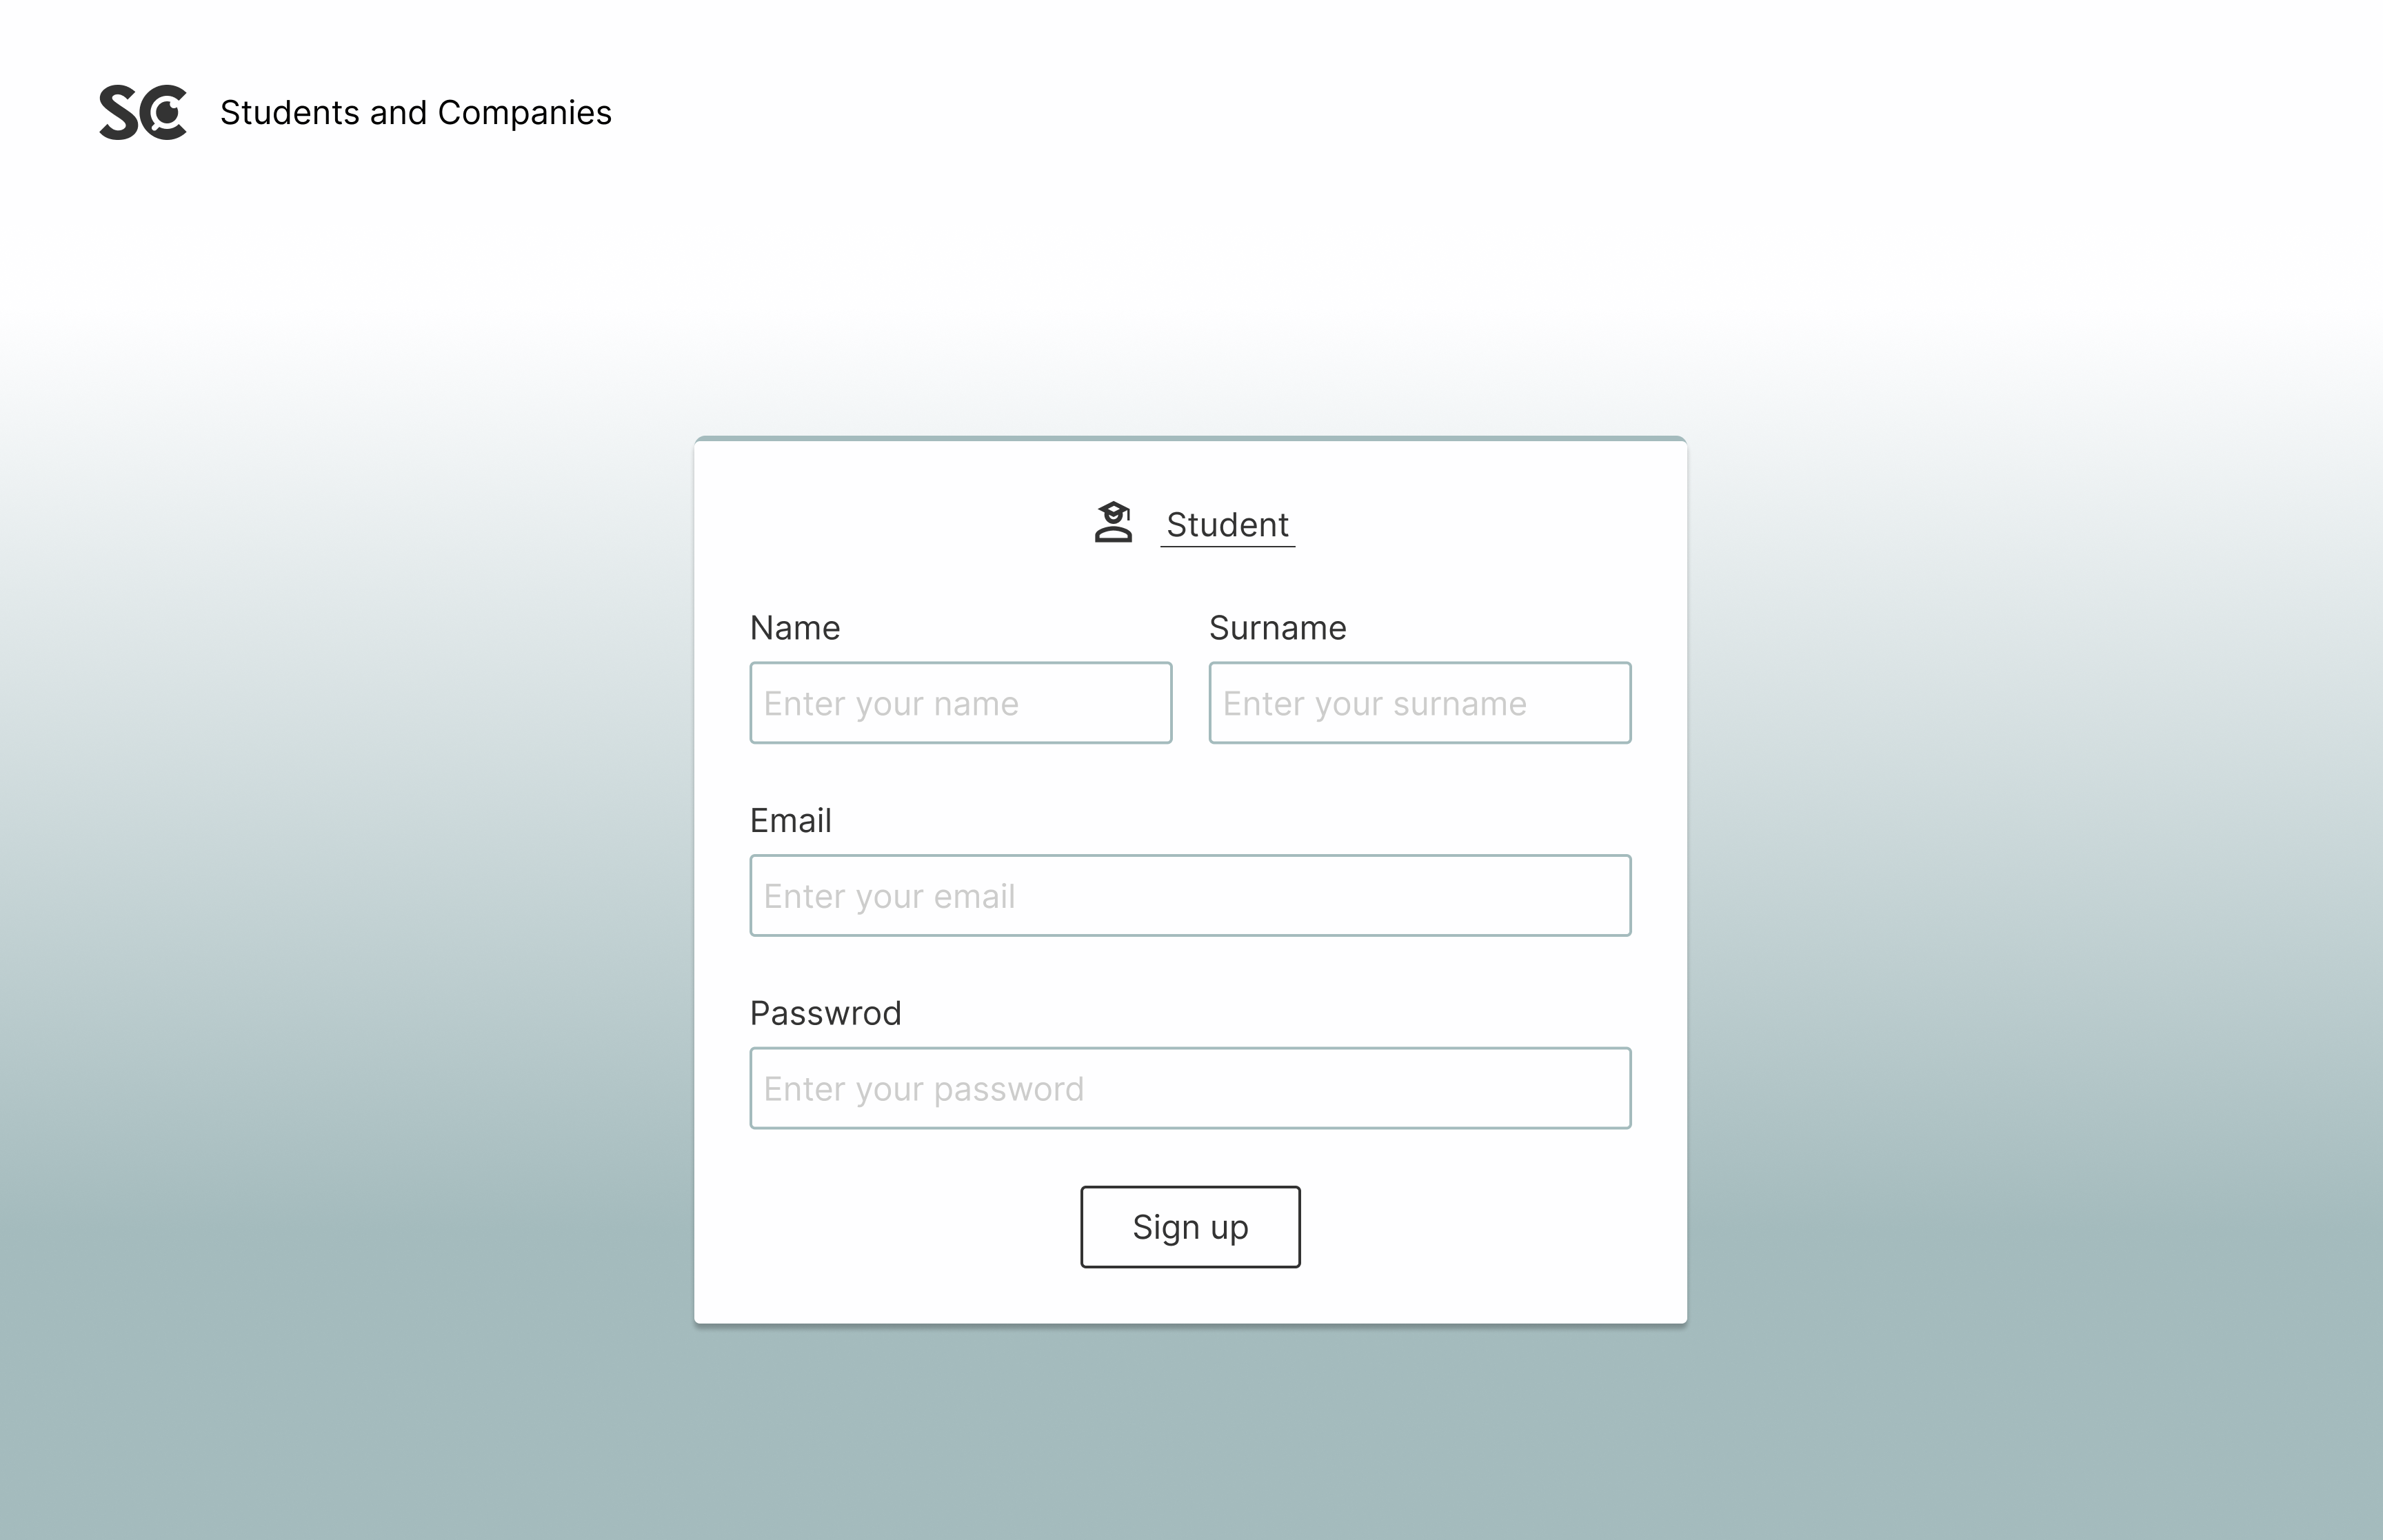
\includegraphics[width=0.8\textwidth]{Images/ui/Student Sign Up}
%    \caption{Student Sign Up}
%    \label{fig:signupStudent}
%\end{figure}
%
%\begin{figure}[H]
%    \centering
%    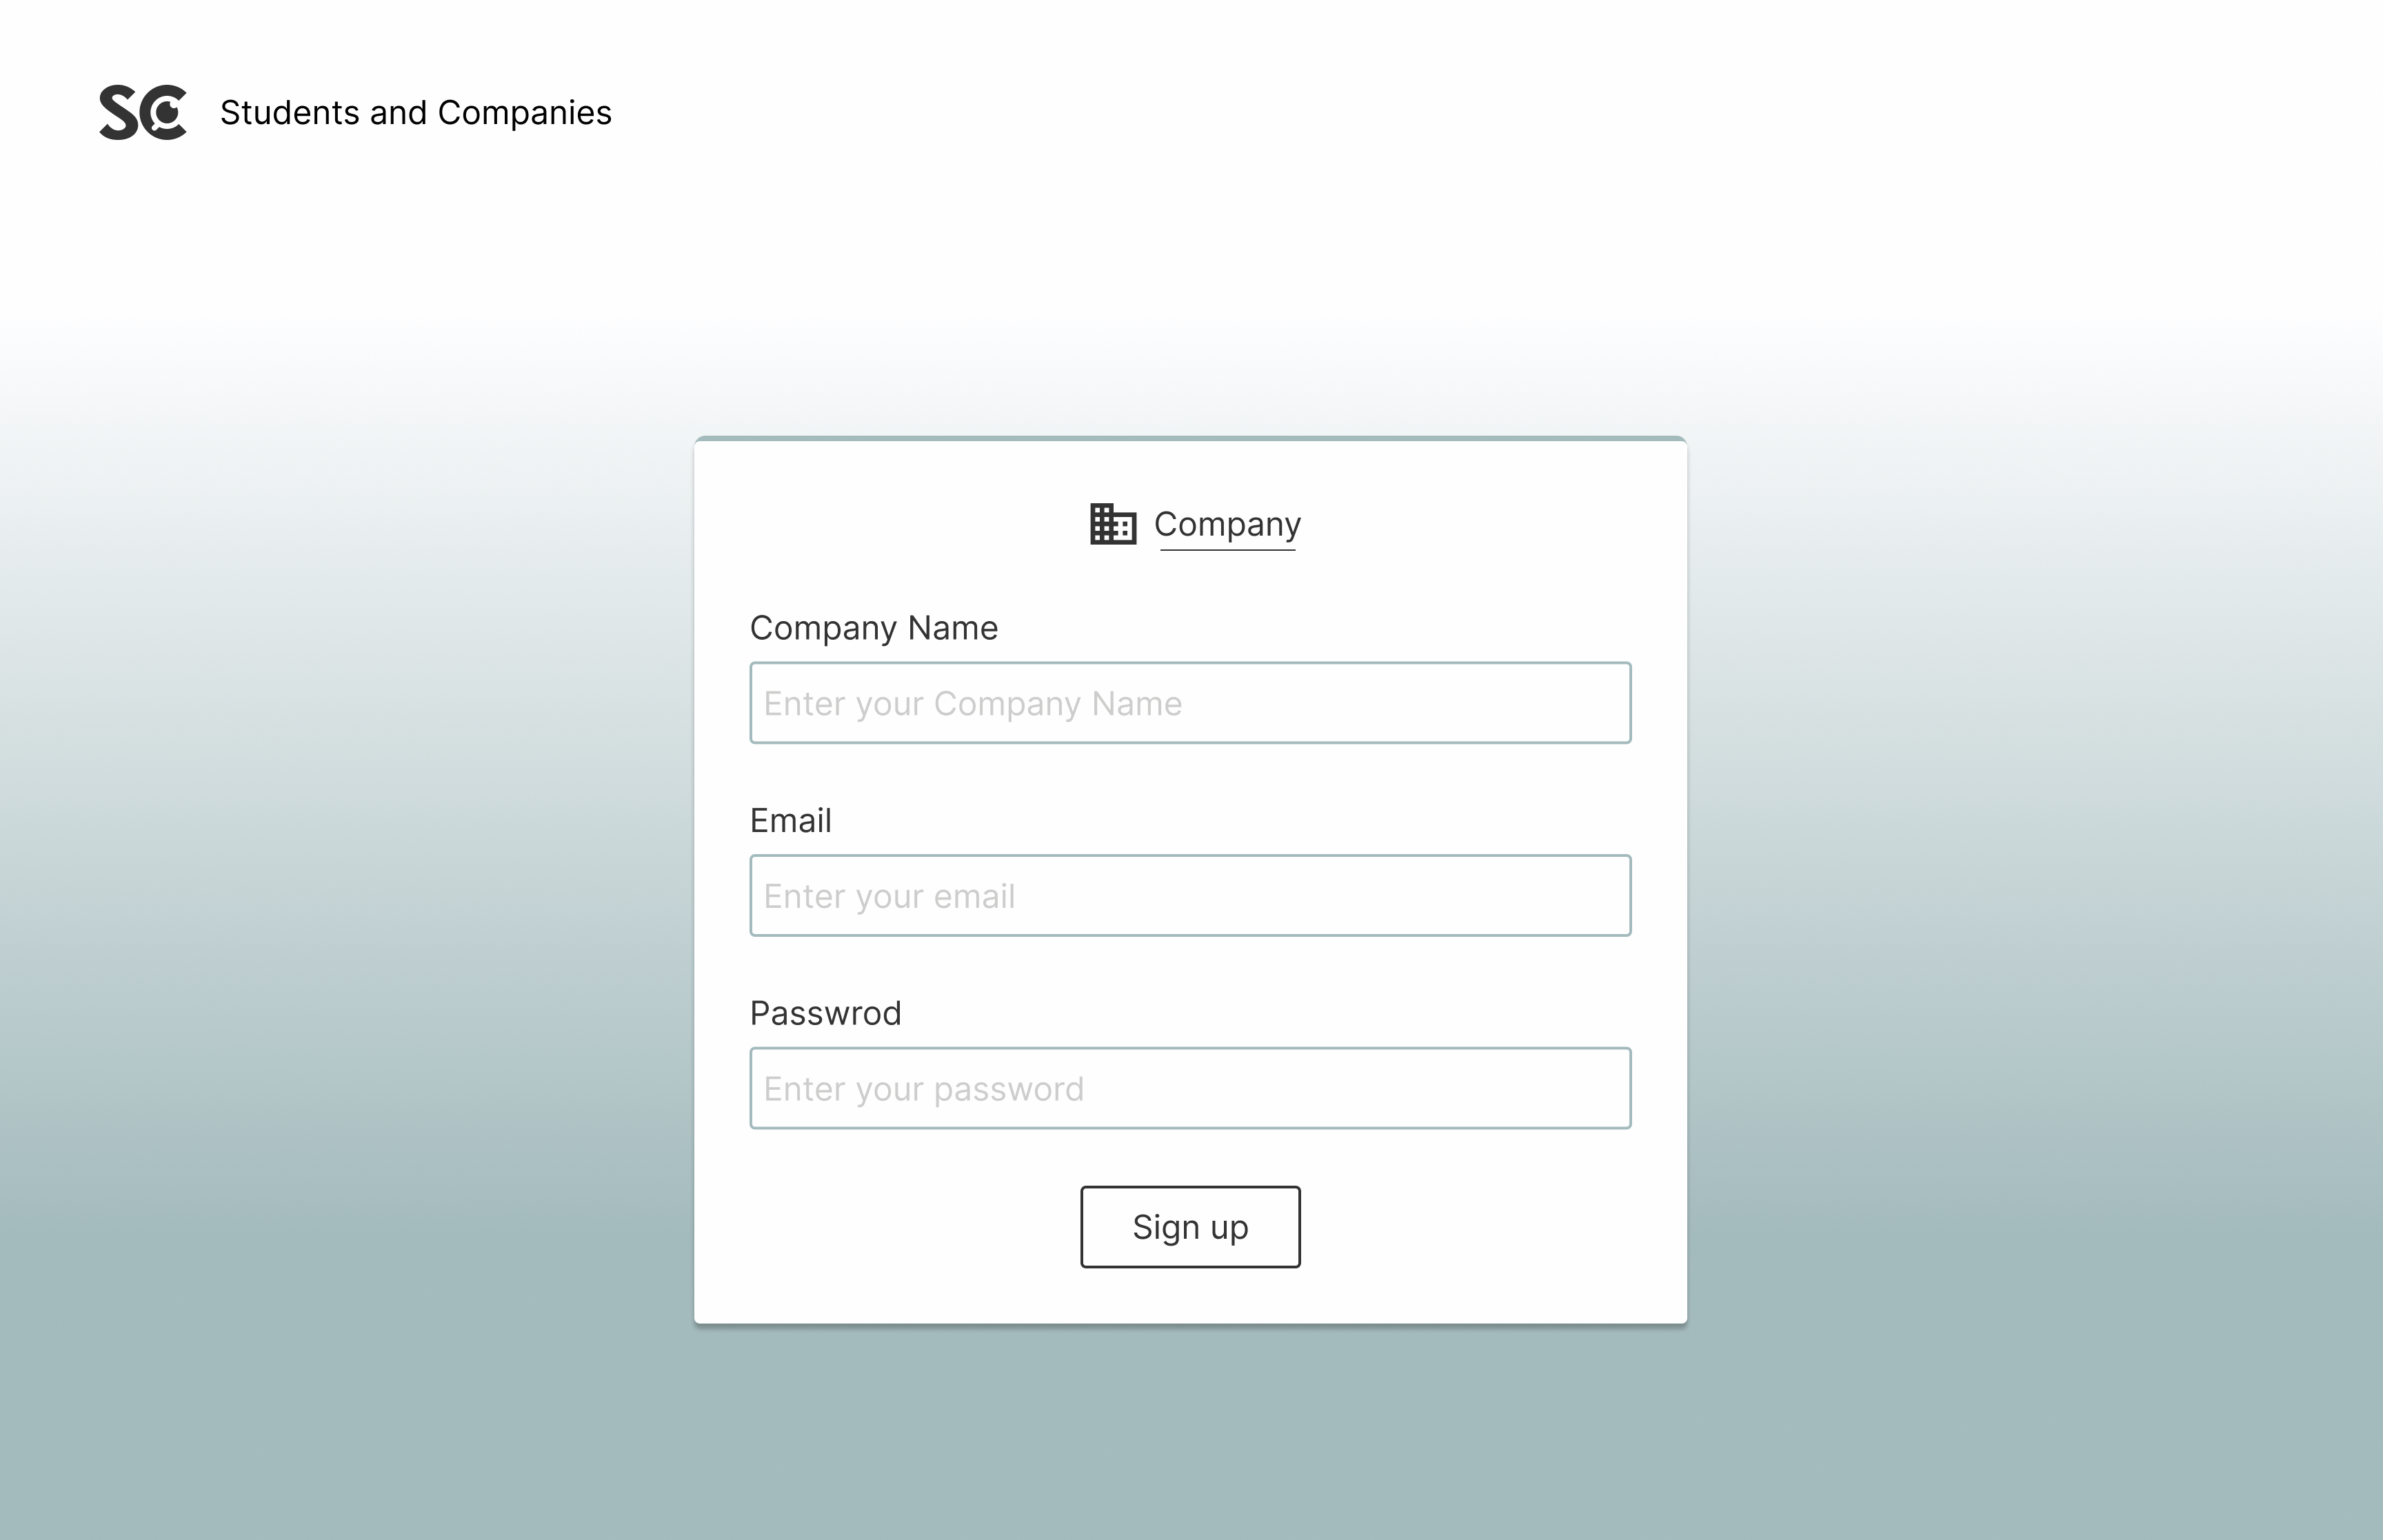
\includegraphics[width=0.8\textwidth]{Images/ui/Company Sign Up}
%    \caption{Company Sign Up}
%    \label{fig:signupCompany}
%\end{figure}
%\begin{figure}[H]
%    \centering
%    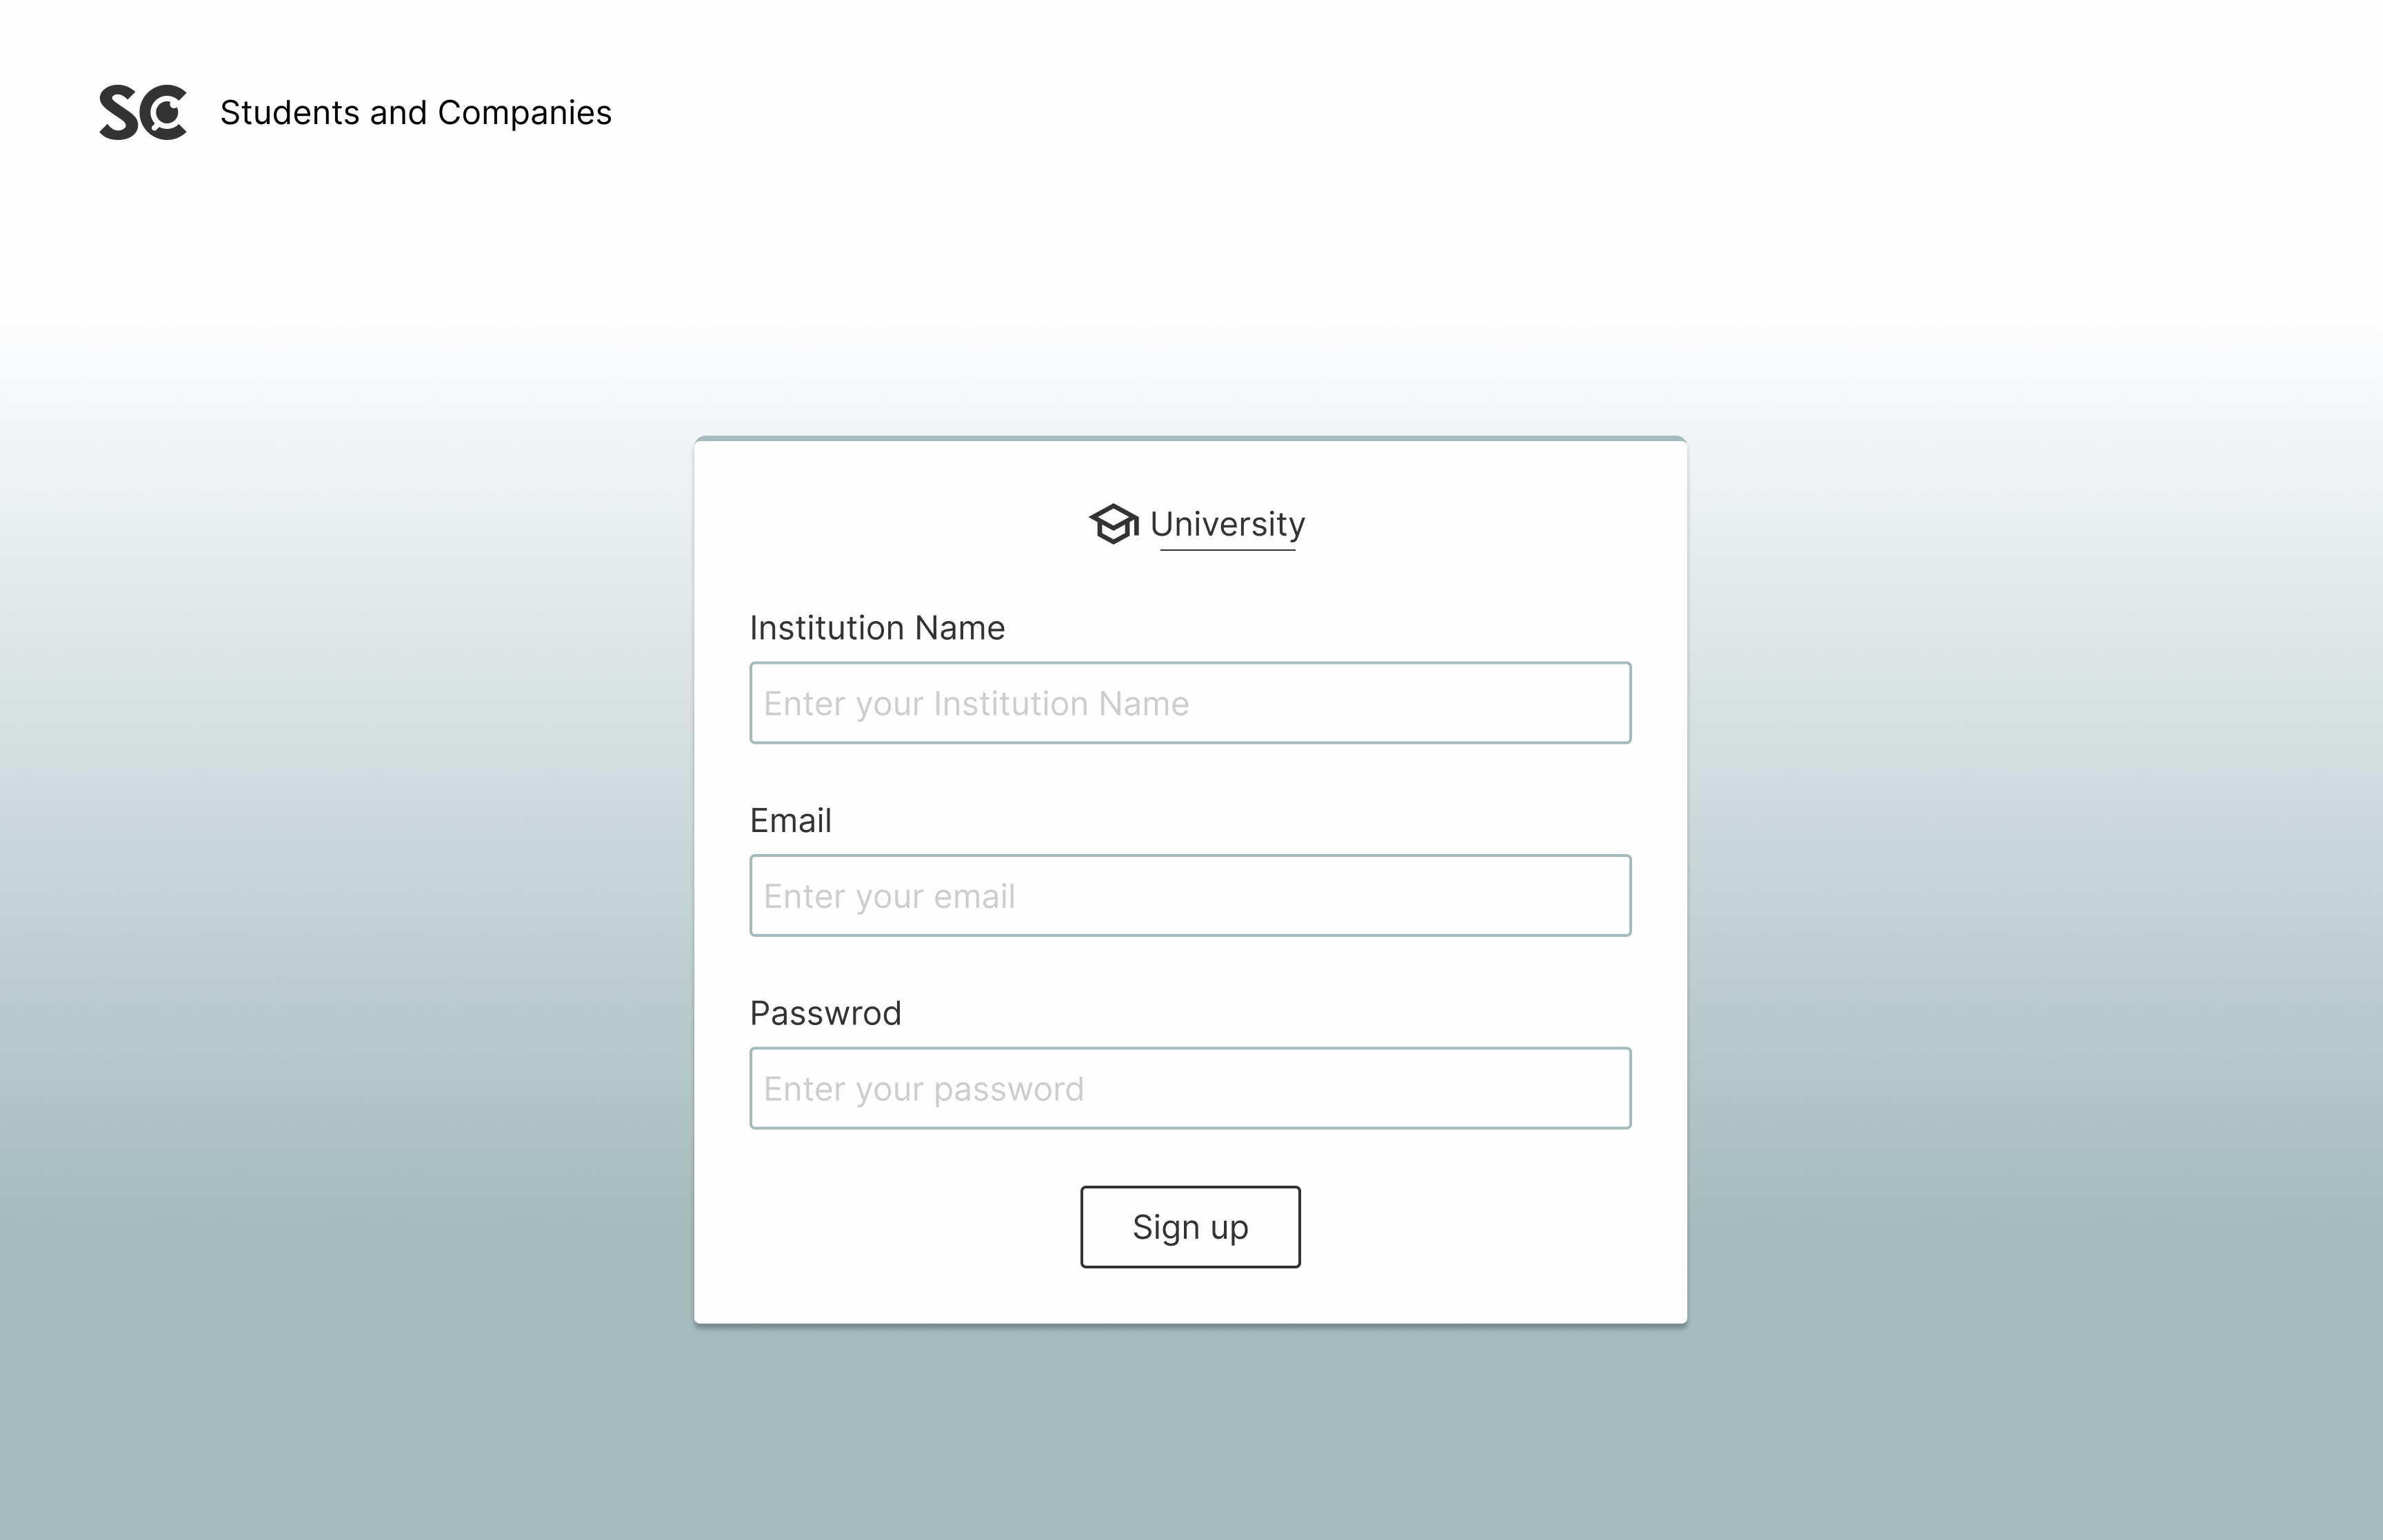
\includegraphics[width=0.8\textwidth]{Images/ui/University Sign Up}
%    \caption{University Sign Up}
%    \label{fig:signupUni}
%\end{figure}
%
%Once we filled in the form and clicked on the Sign Up button, if the information is correct, we are going to receive a confirmation email and the following interface is shown.
%\begin{figure}[H]
%    \centering
%    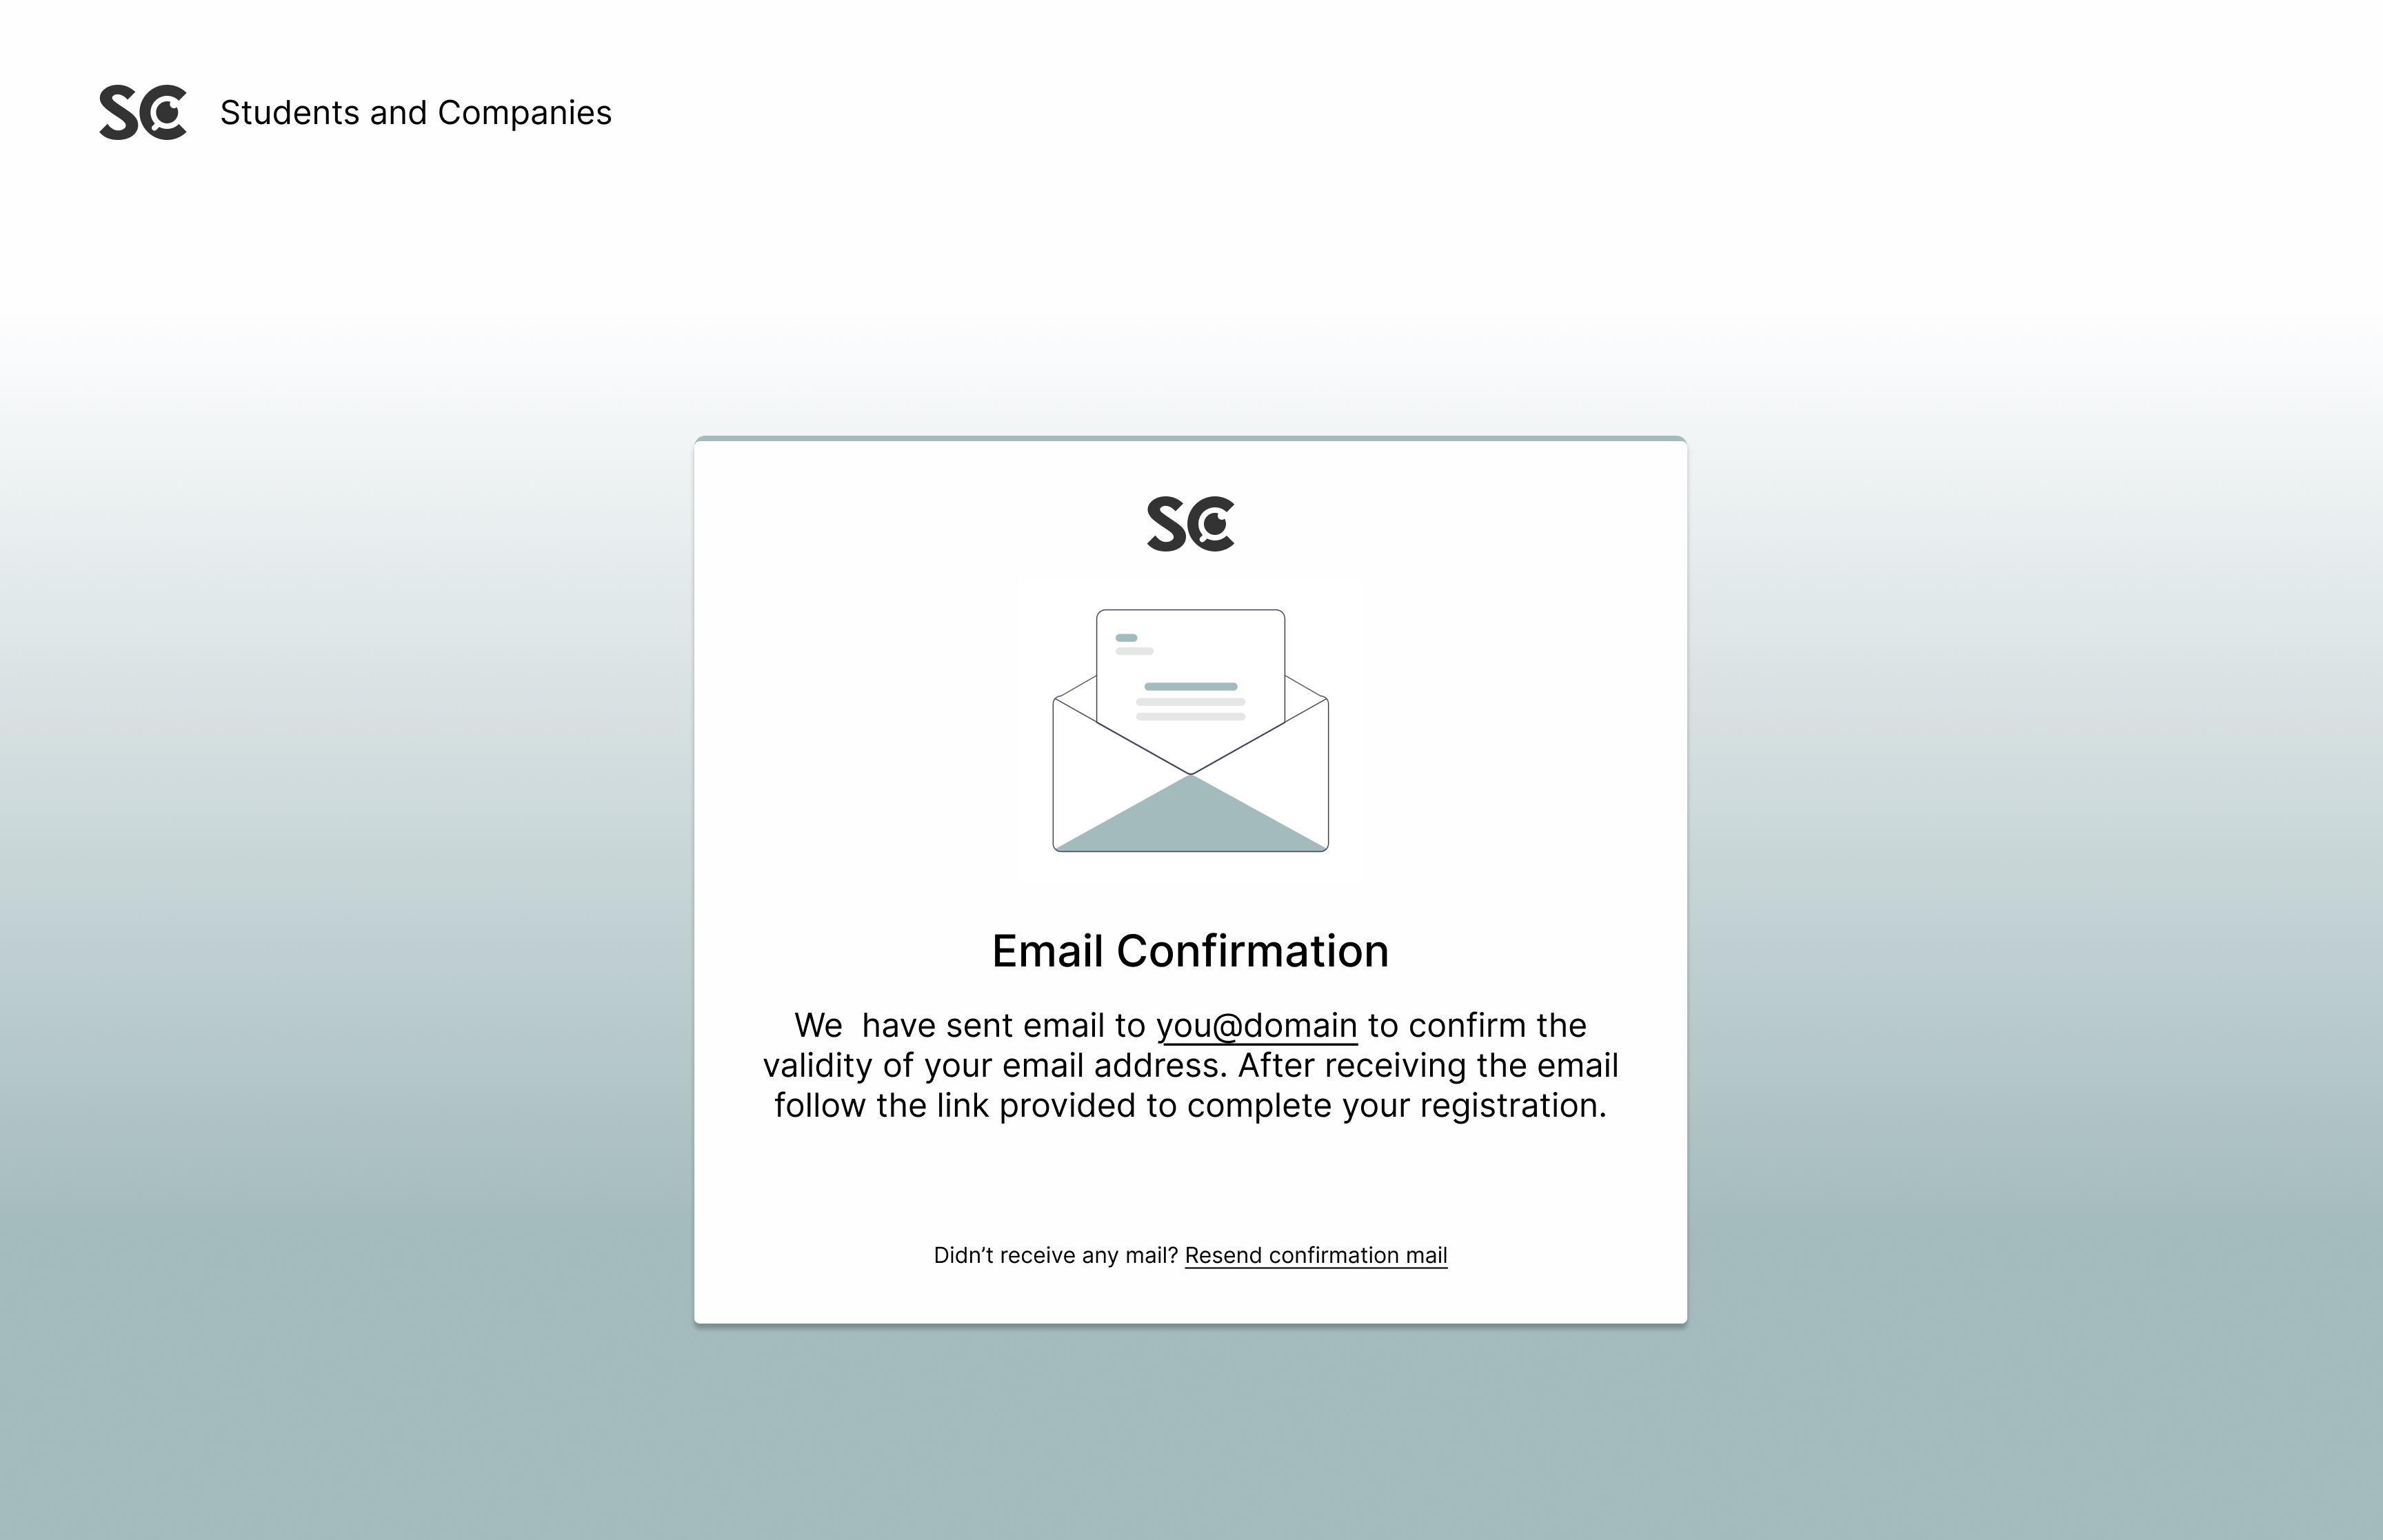
\includegraphics[width=0.8\textwidth]{Images/ui/Confirmation Email}
%    \caption{Confirmation Email Sent}
%    \label{fig:confirmEmail}
%\end{figure}
%Once we follow the link we are going to get the successful verification, as illustrated in the next image.
%\begin{figure}[H]
%    \centering
%    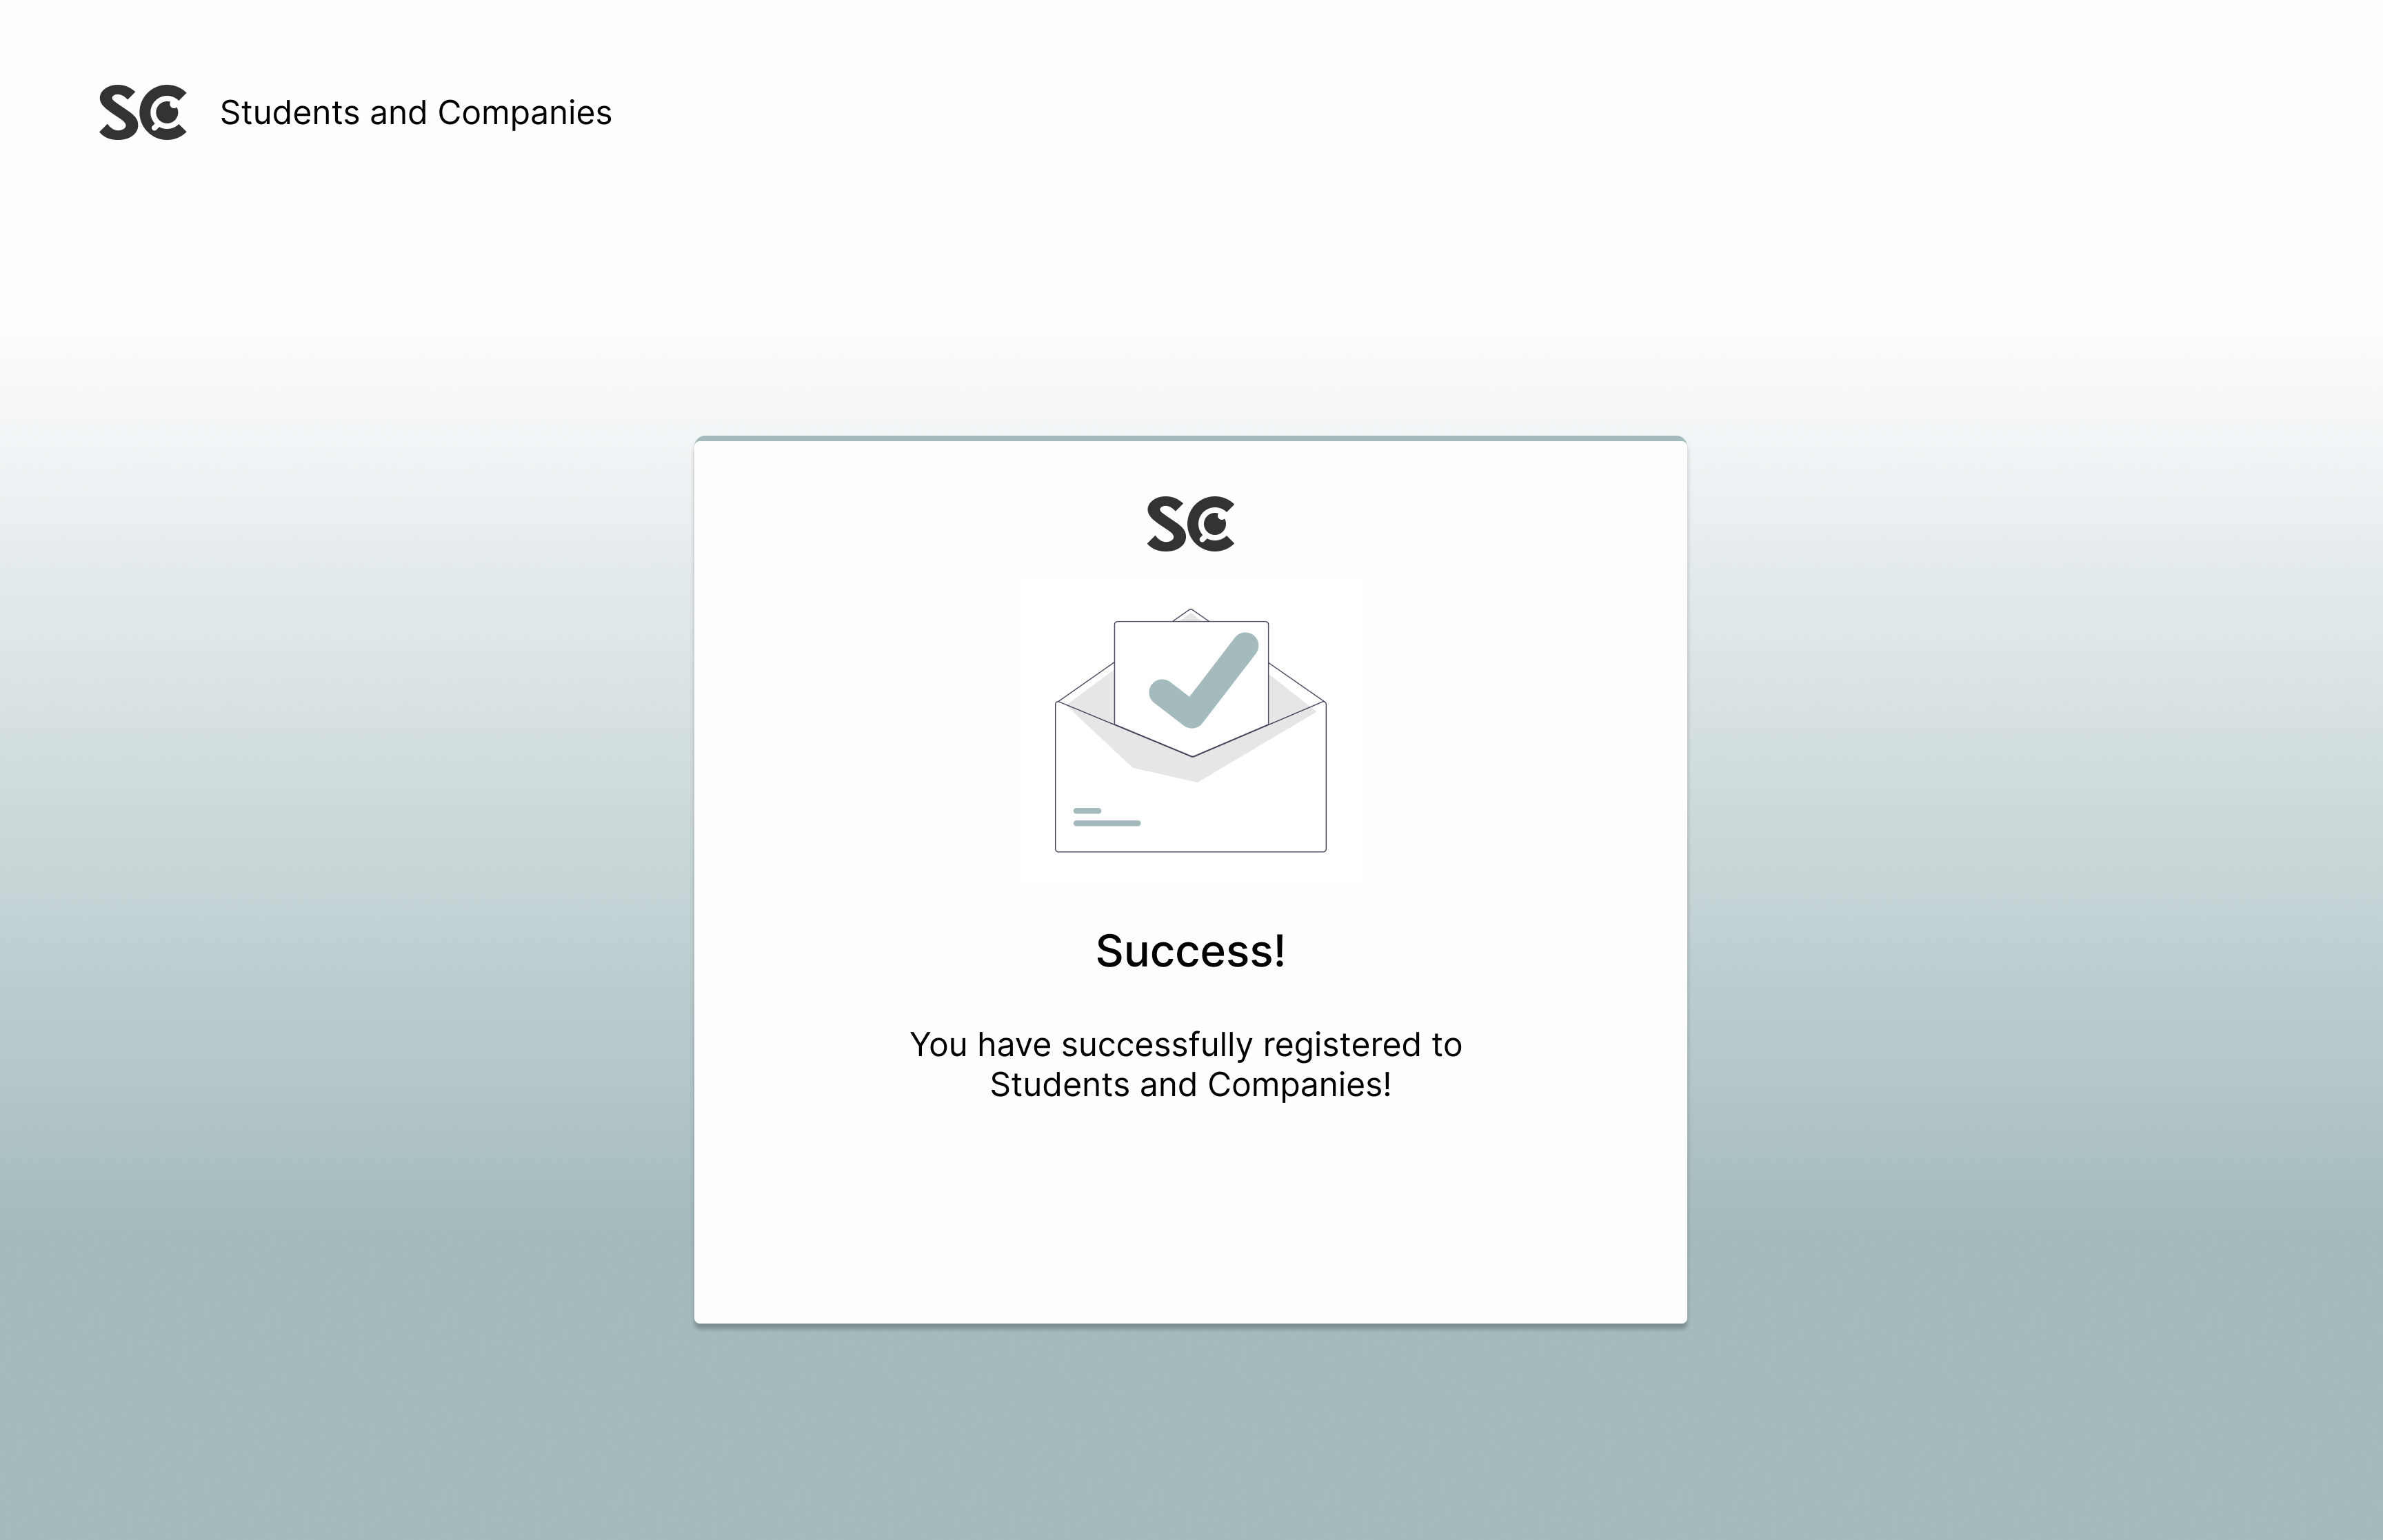
\includegraphics[width=0.8\textwidth]{Images/ui/Confirmation Email 2}
%    \caption{Success!}
%    \label{fig:confirmSuccess}
%\end{figure}
%
%Once we are done with the registration process, we can finally login.
%To do so we can go to the landing page and, in the top right, click on the Log In button.
%The log in interface is as follows.
%\begin{figure}[H]
%    \centering
%    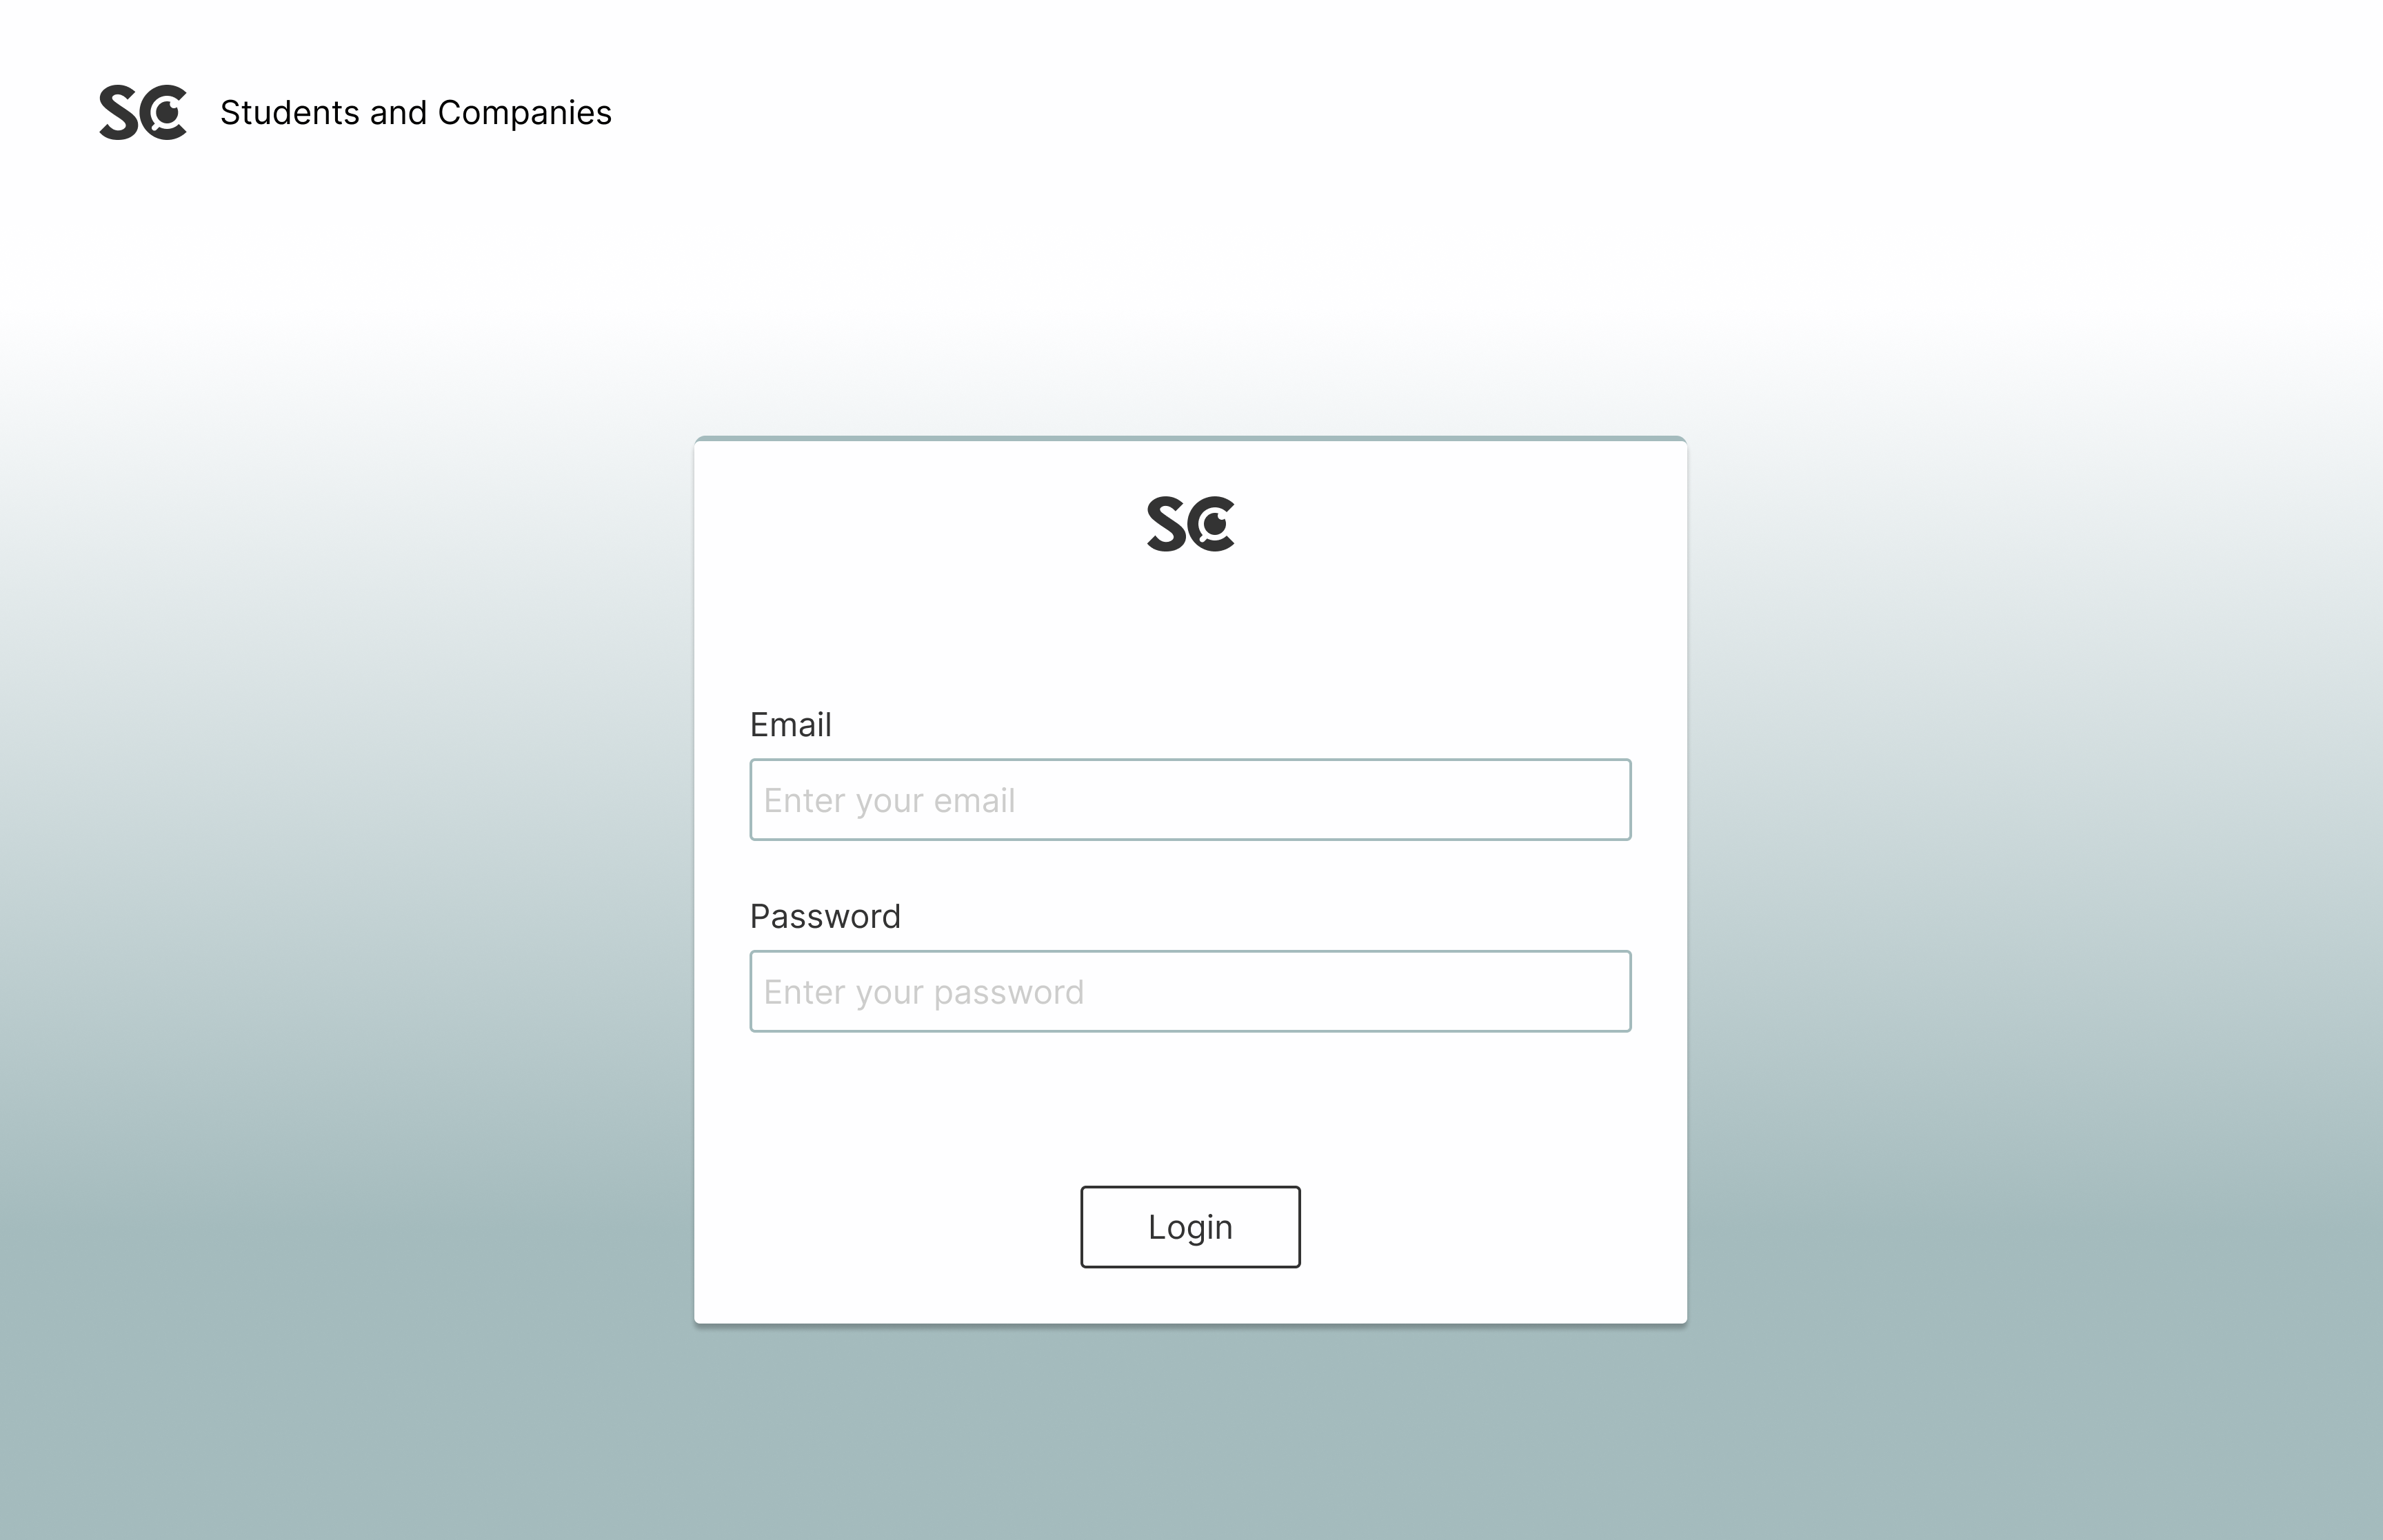
\includegraphics[width=0.8\textwidth]{Images/ui/Login}
%    \caption{Log In}
%    \label{fig:login}
%\end{figure}
%
%If we successfully compiled the form and we clicked on the Log In button, we are going to get redirected to the home page, which is different for every type of user that the platform can have.
%In the following sections, we are going to depict the different interfaces based on which user we are considering: Student, Company or University.
%
%\section{Student Interface}\label{sec:student-interface}
%Here we present the User Interface for a Student.
%If it's the first time that the Student has logged in, then the Upload CV interface is shown, since it's a fundamental step to be able to find and internship.
%The process is pretty simple, just click on the icon, upload your CV and press the button.
%\begin{figure}[H]
%    \centering
%    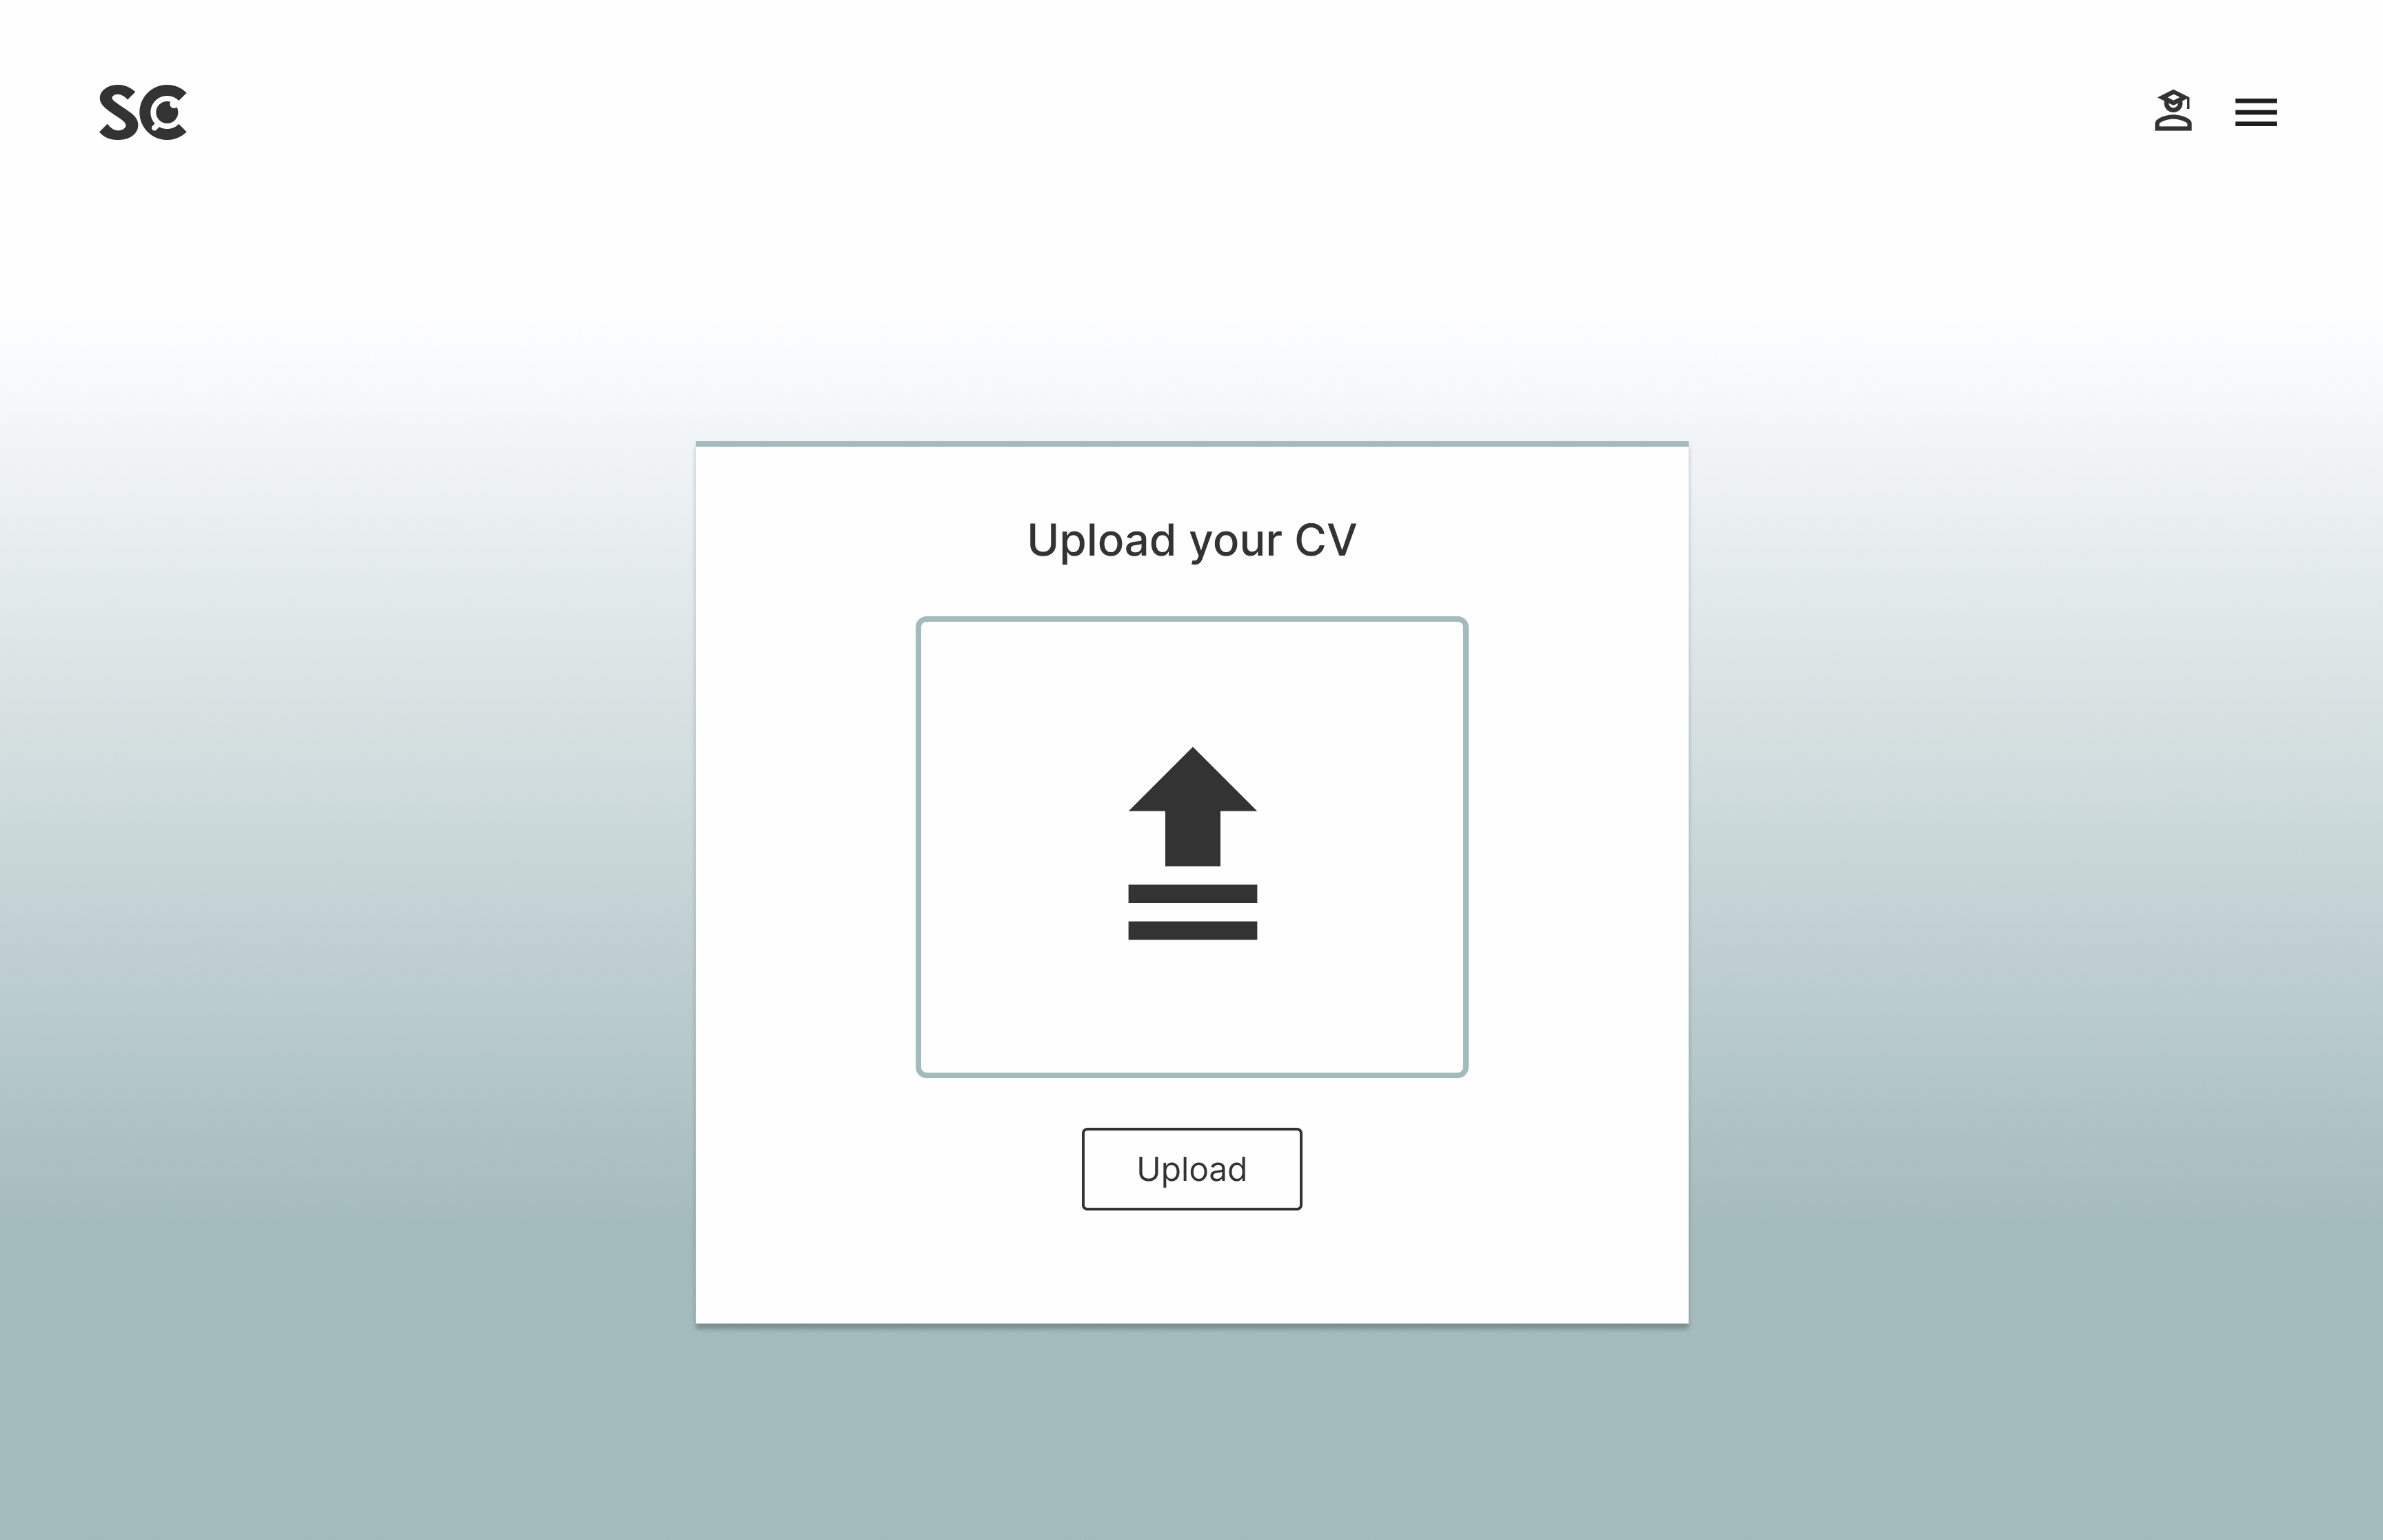
\includegraphics[width=0.8\textwidth]{Images/ui/Upload CV}
%    \caption{Upload CV}
%    \label{fig:uploadcv}
%\end{figure}
%Once we are done uploading the CV, we are going to be presented with a suggestion box, that contains all the best guidelines and actual suggestions that are tailored by the system depending on the Student CV using the AnalysisTool.
%\begin{figure}[H]
%    \centering
%    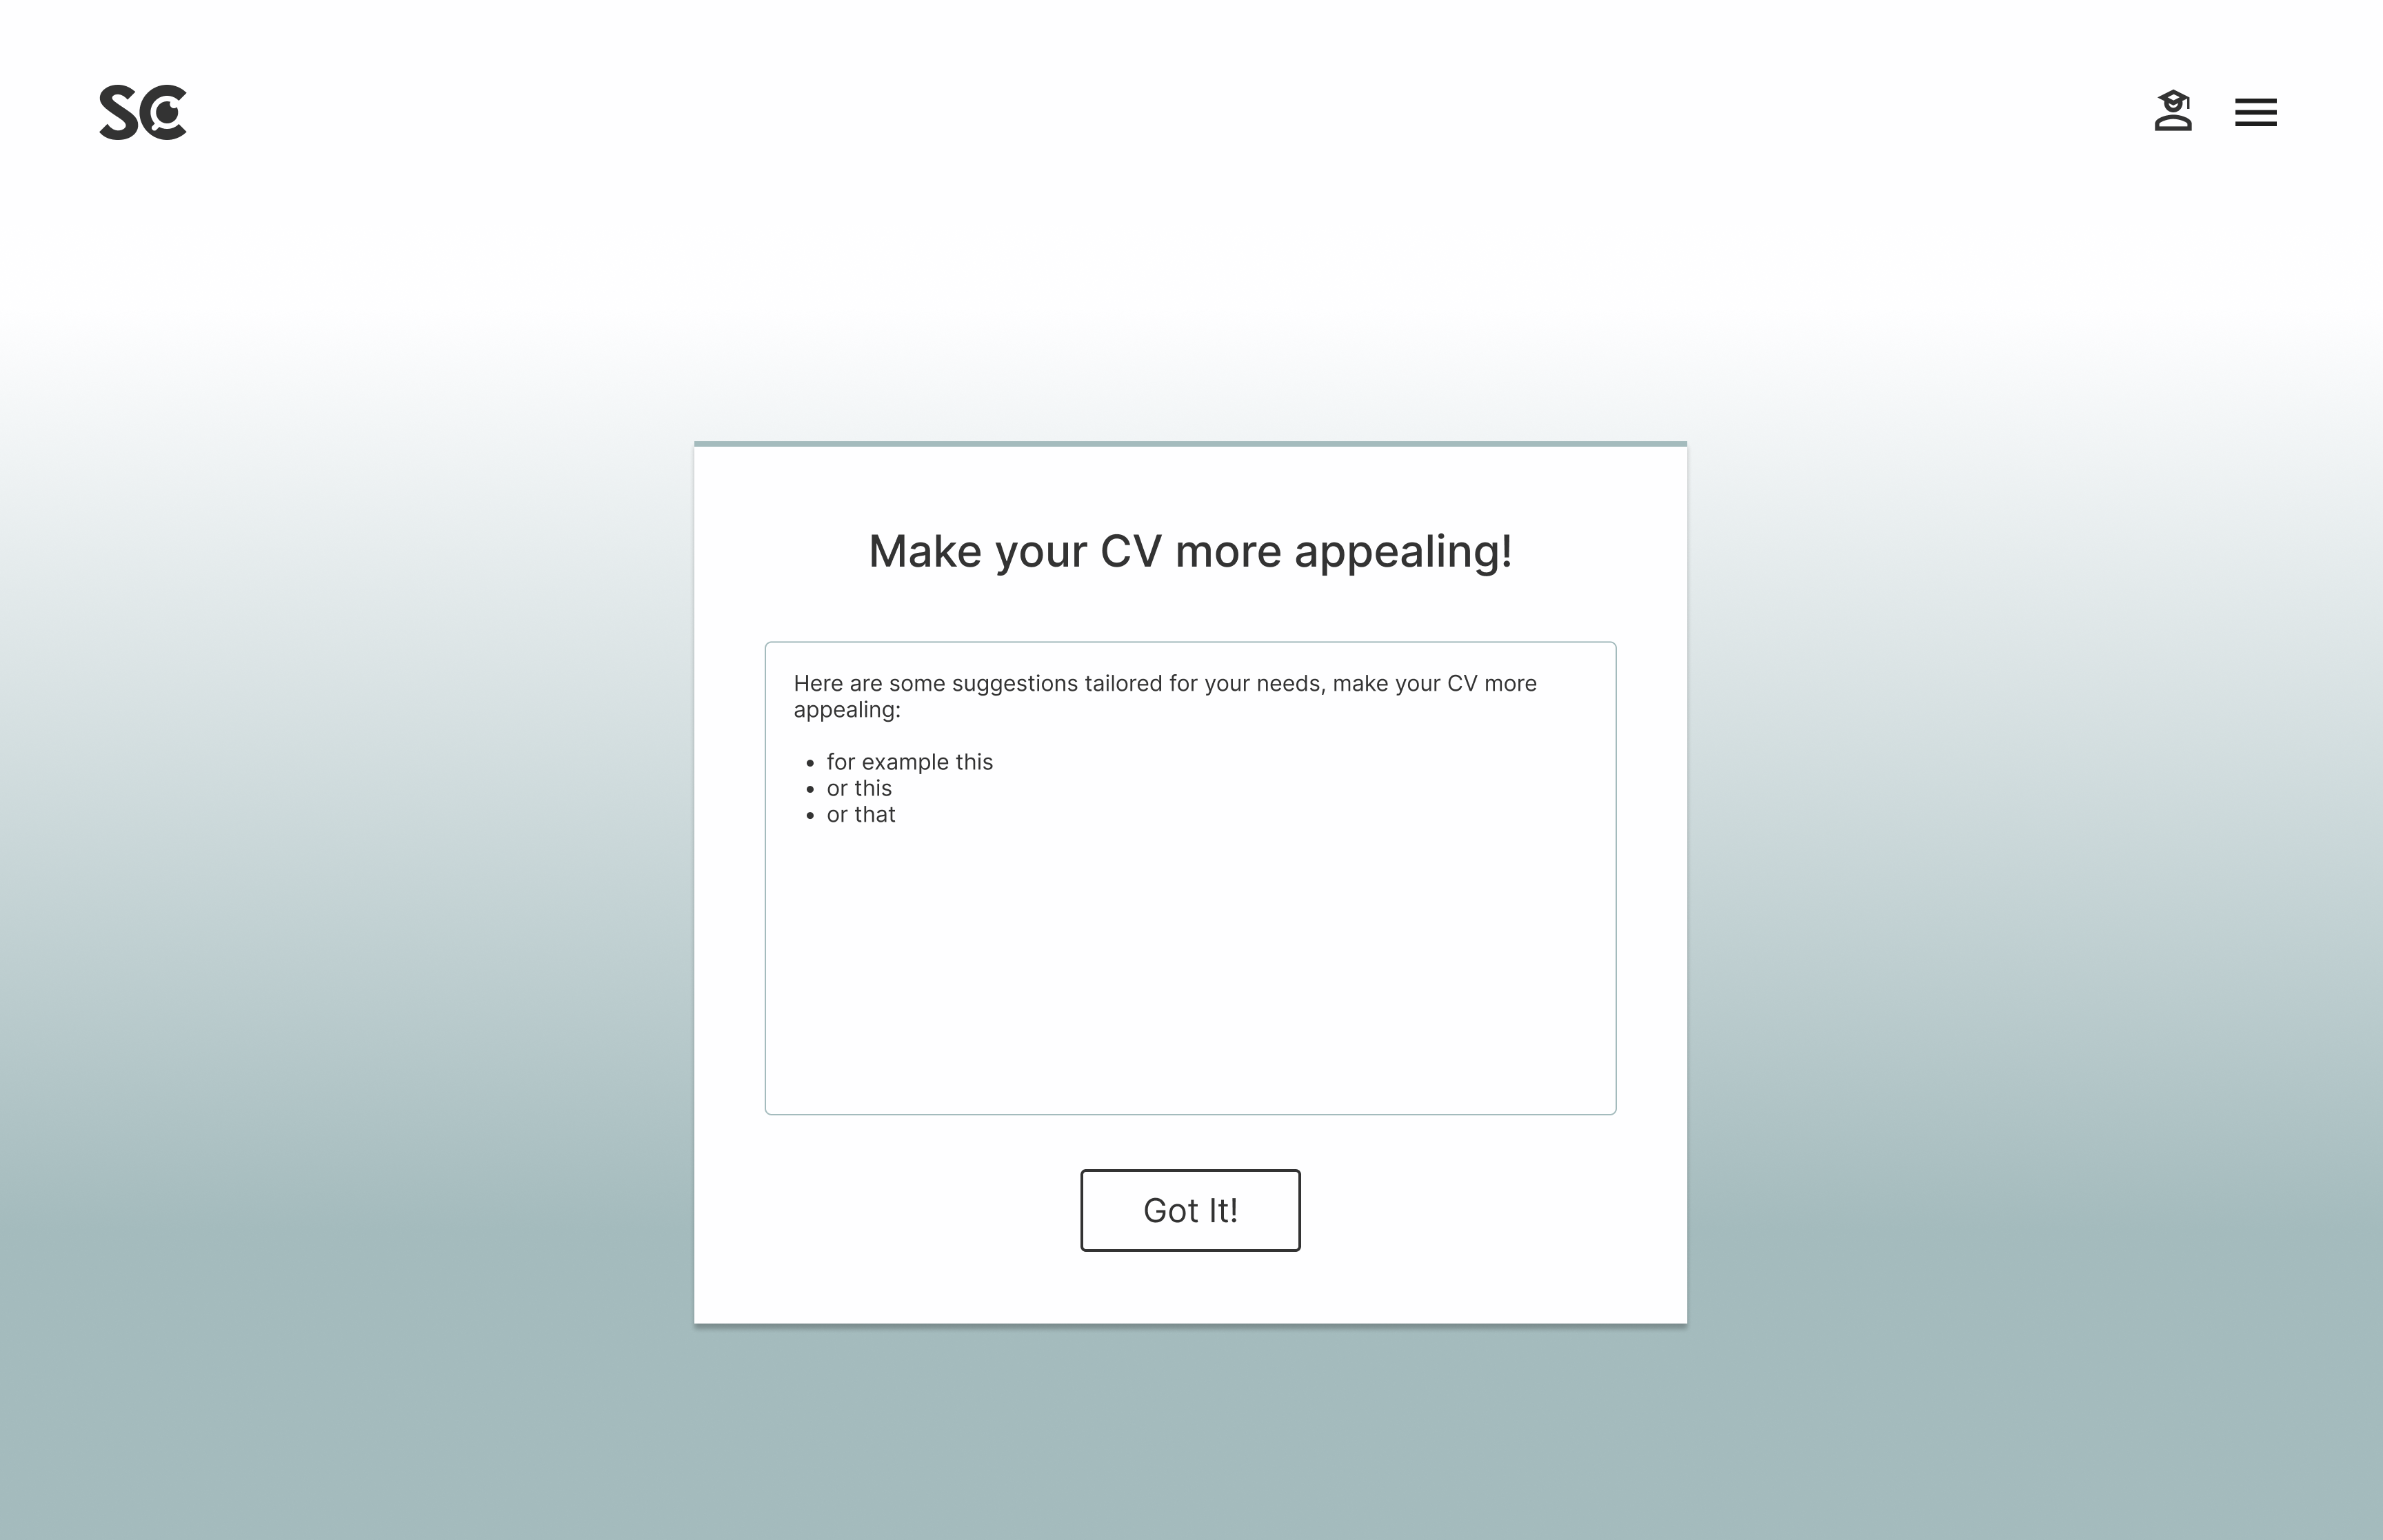
\includegraphics[width=0.8\textwidth]{Images/ui/Suggestions on CV}
%    \caption{CV Suggestions}
%    \label{fig:suggestionCV}
%\end{figure}
%
%After successfully uploading the CV, and every time will log in in the future, we are presented with the home page, in this case it's the View Available Internships page, since the first thing a student might want to do is to find an internship.
%The page is structured as follows:
%\begin{itemize}
%    \item On the left hand side, we are presented with the list of all the available internships, that we can filter by using the search box on the top left.
%    \item The selected internship, that we can see by the black accent on top of the item box, is displayed in detail on the right part of the interface.
%    \item In the detail section, we can find all information ranging from skills, benefits, description and so on. We can also use the sidebar to scroll further down the detail box, if the content does not fit on the screen.
%    \item In the detail section we have the Apply button, that can be used to apply for the selected internship.
%    \item On the top right we can find a button that redirects us to the recommended internships page.
%\end{itemize}
%\begin{figure}[H]
%    \centering
%    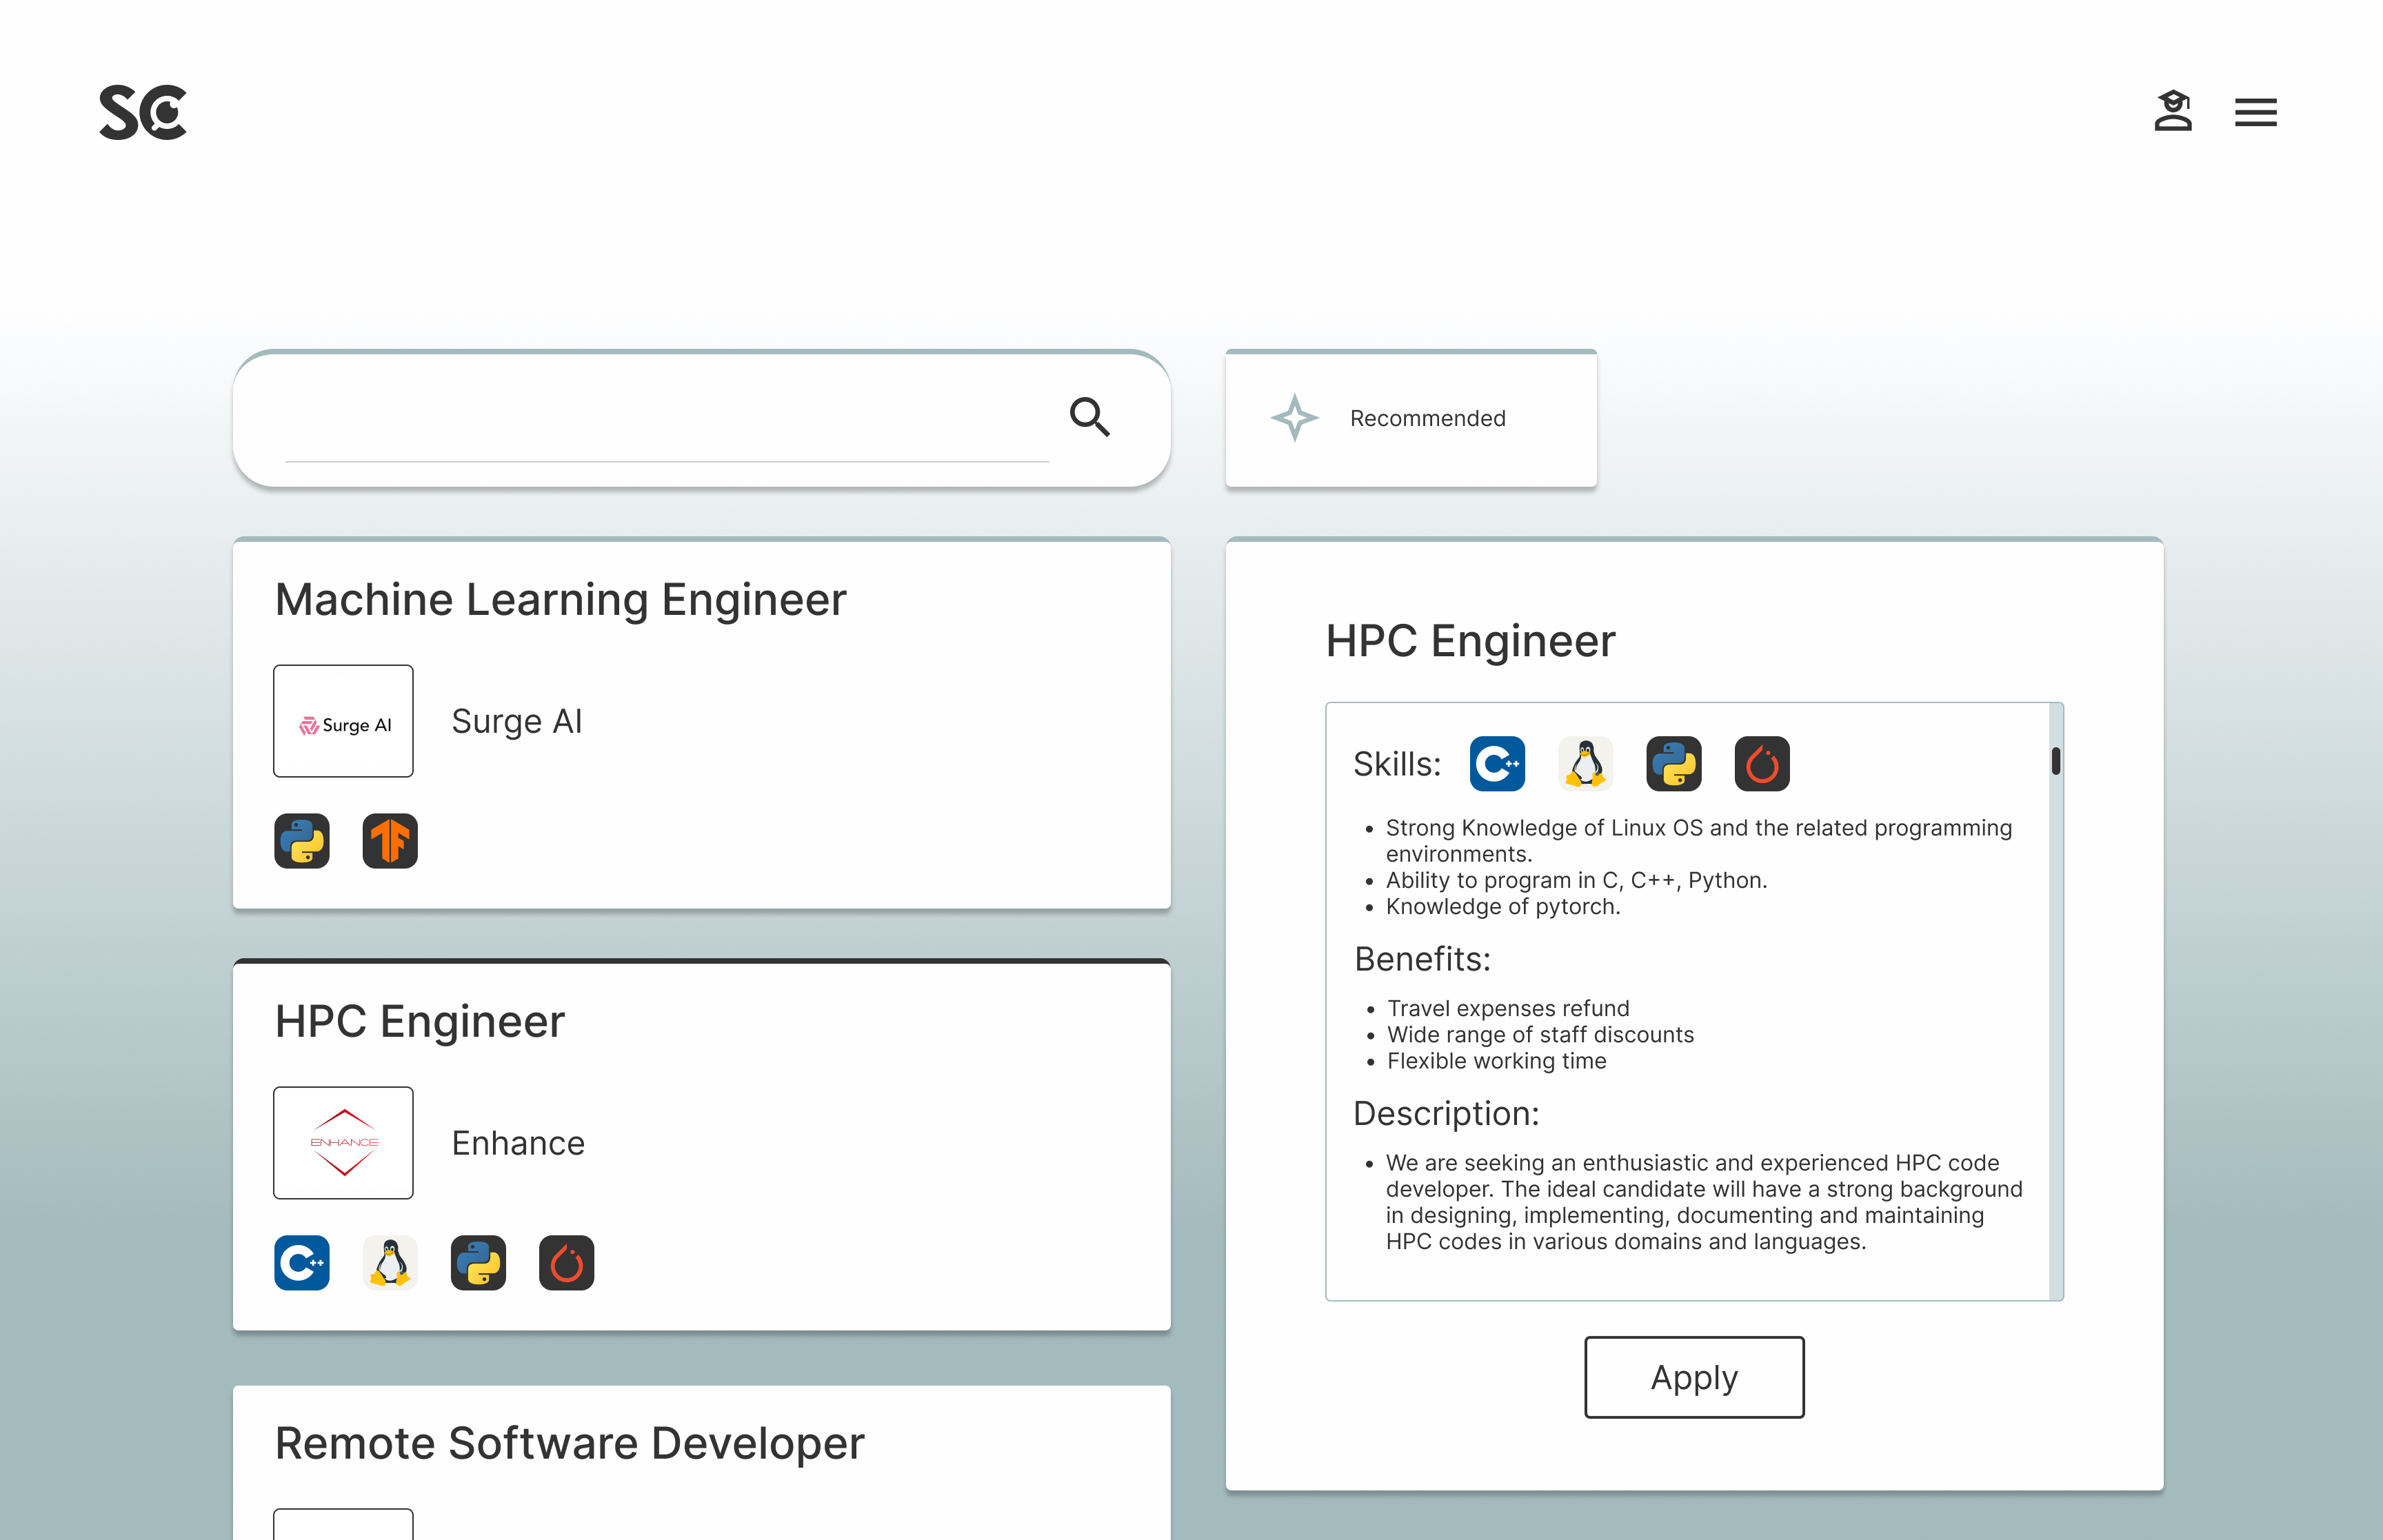
\includegraphics[width=0.8\textwidth]{Images/ui/View Internships}
%    \caption{View Available Internships (HOME)}
%    \label{fig:homeStuednt}
%\end{figure}
%
%The following picture represents the Recommended Internships page, and as we can see it's basically the same as the previous one apart from the different list of displayed internship and the button on the top right for the recommendation that is selected.
%\begin{figure}[H]
%    \centering
%    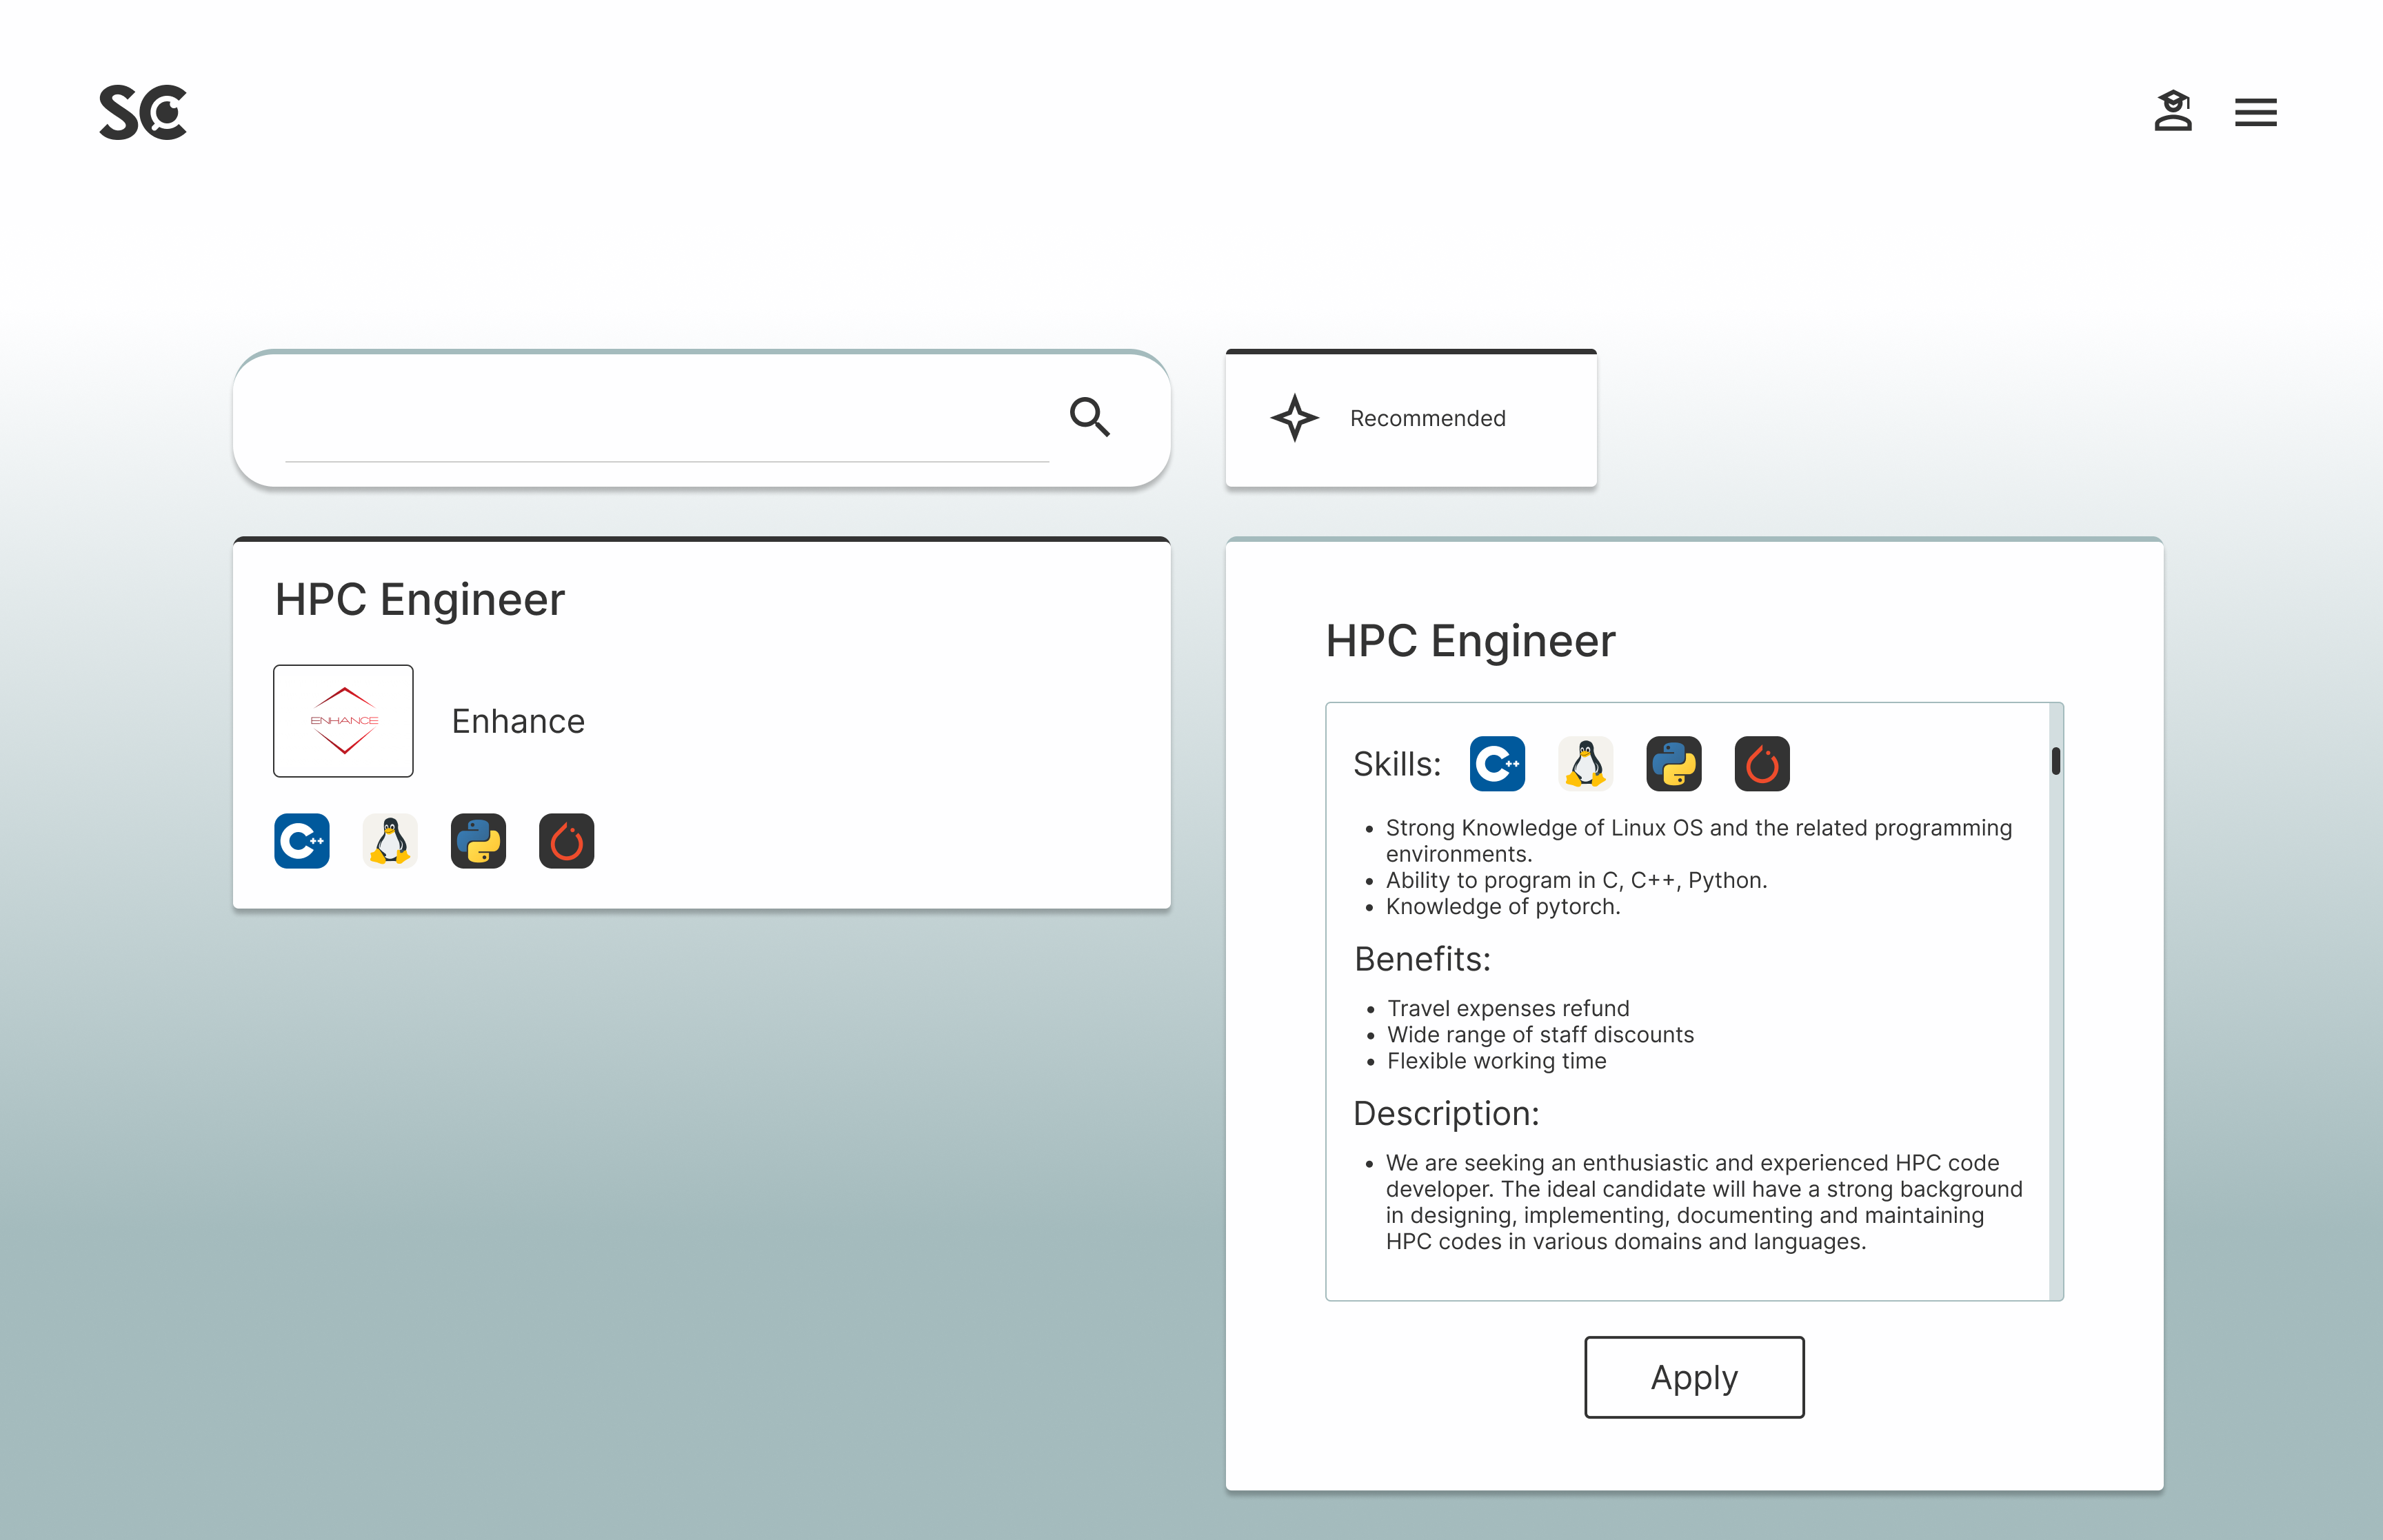
\includegraphics[width=0.8\textwidth]{Images/ui/View recommended internships}
%    \caption{View Recommended Internships }
%    \label{fig:recommendedInternships}
%\end{figure}
%
%Let's assume we received some notifications, then the Inbox is where we can find and manage those: from the basic ones to offers that we might receive or the responses of the University that manages our internships.
%Here we can scroll through all the notifications, viewing their content and expressing our choices for offers that we receive.
%\begin{figure}[H]
%    \centering
%    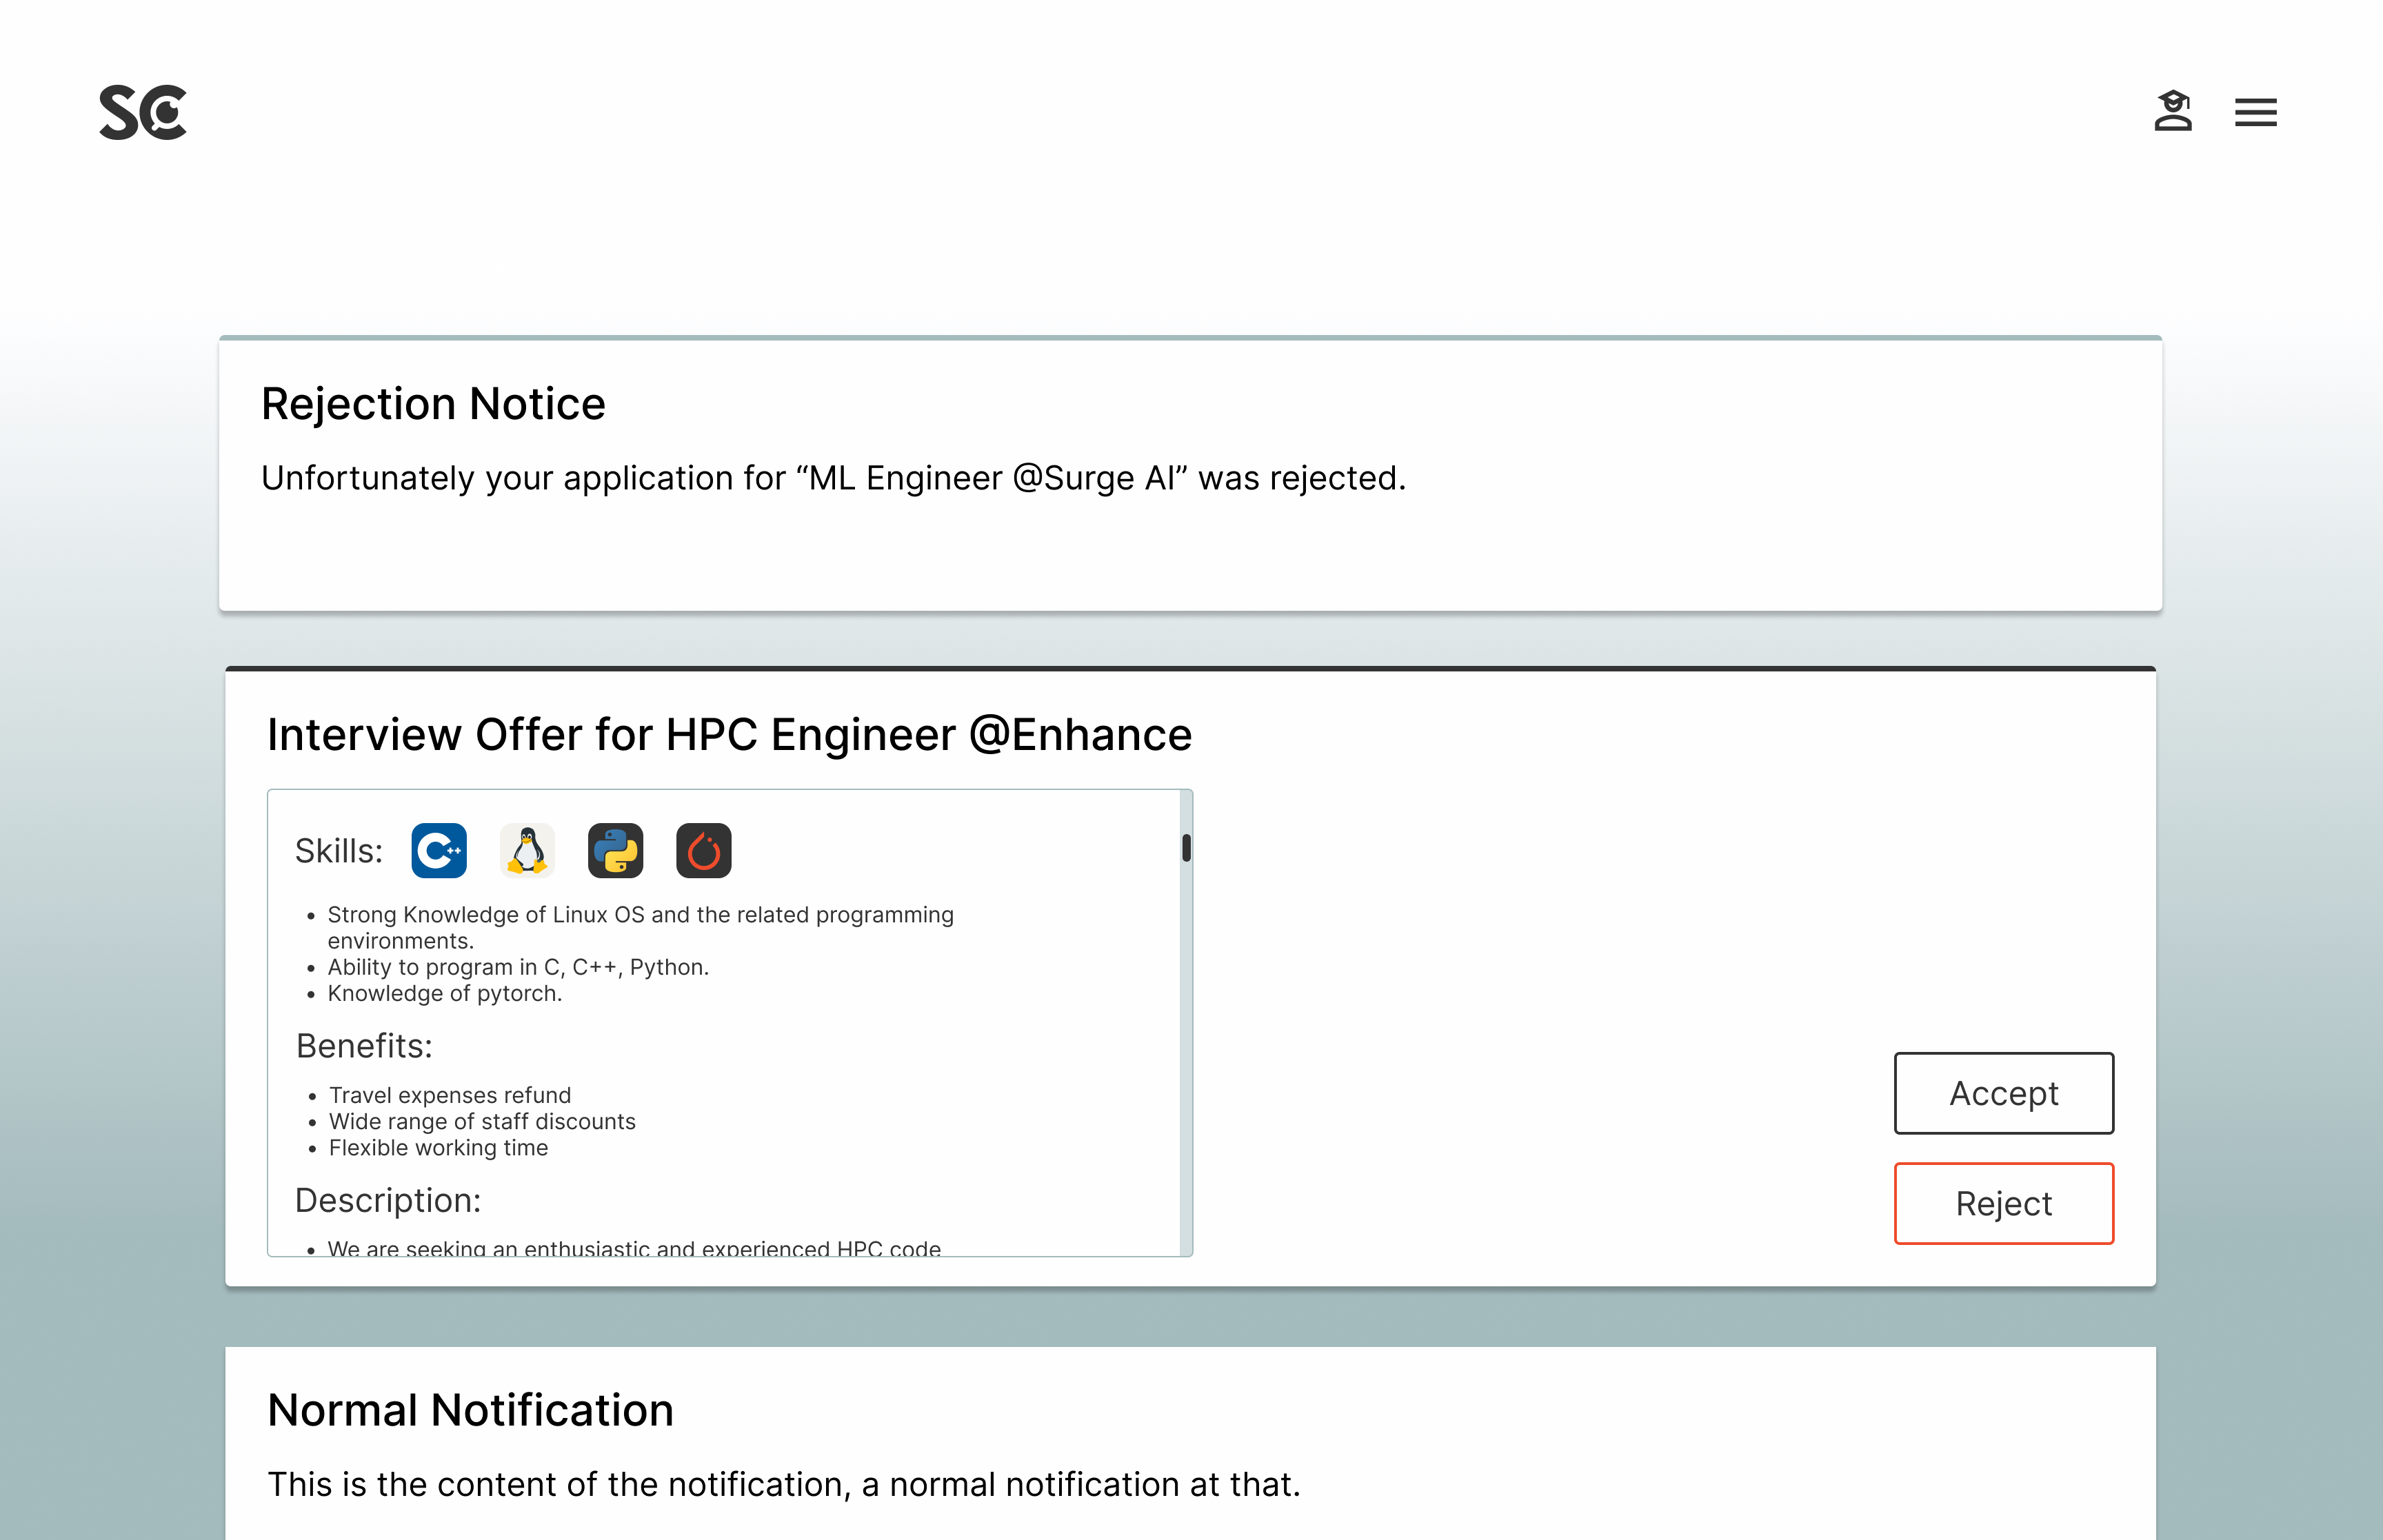
\includegraphics[width=0.8\textwidth]{Images/ui/Consider offer}
%    \caption{Student Inbox}
%    \label{fig:studentInbox}
%\end{figure}
%
%Another interface is the View Planned Interviews, here we can find a list of all the planned interviews and similarly to the home page, we can select each one of them and see on the right hand side the detail: date, time and additional notes.
%On the top left side we can also find a searchbar and a selection box that we can use to further filter the displayed list of planned interviews.
%\begin{figure}[H]
%    \centering
%    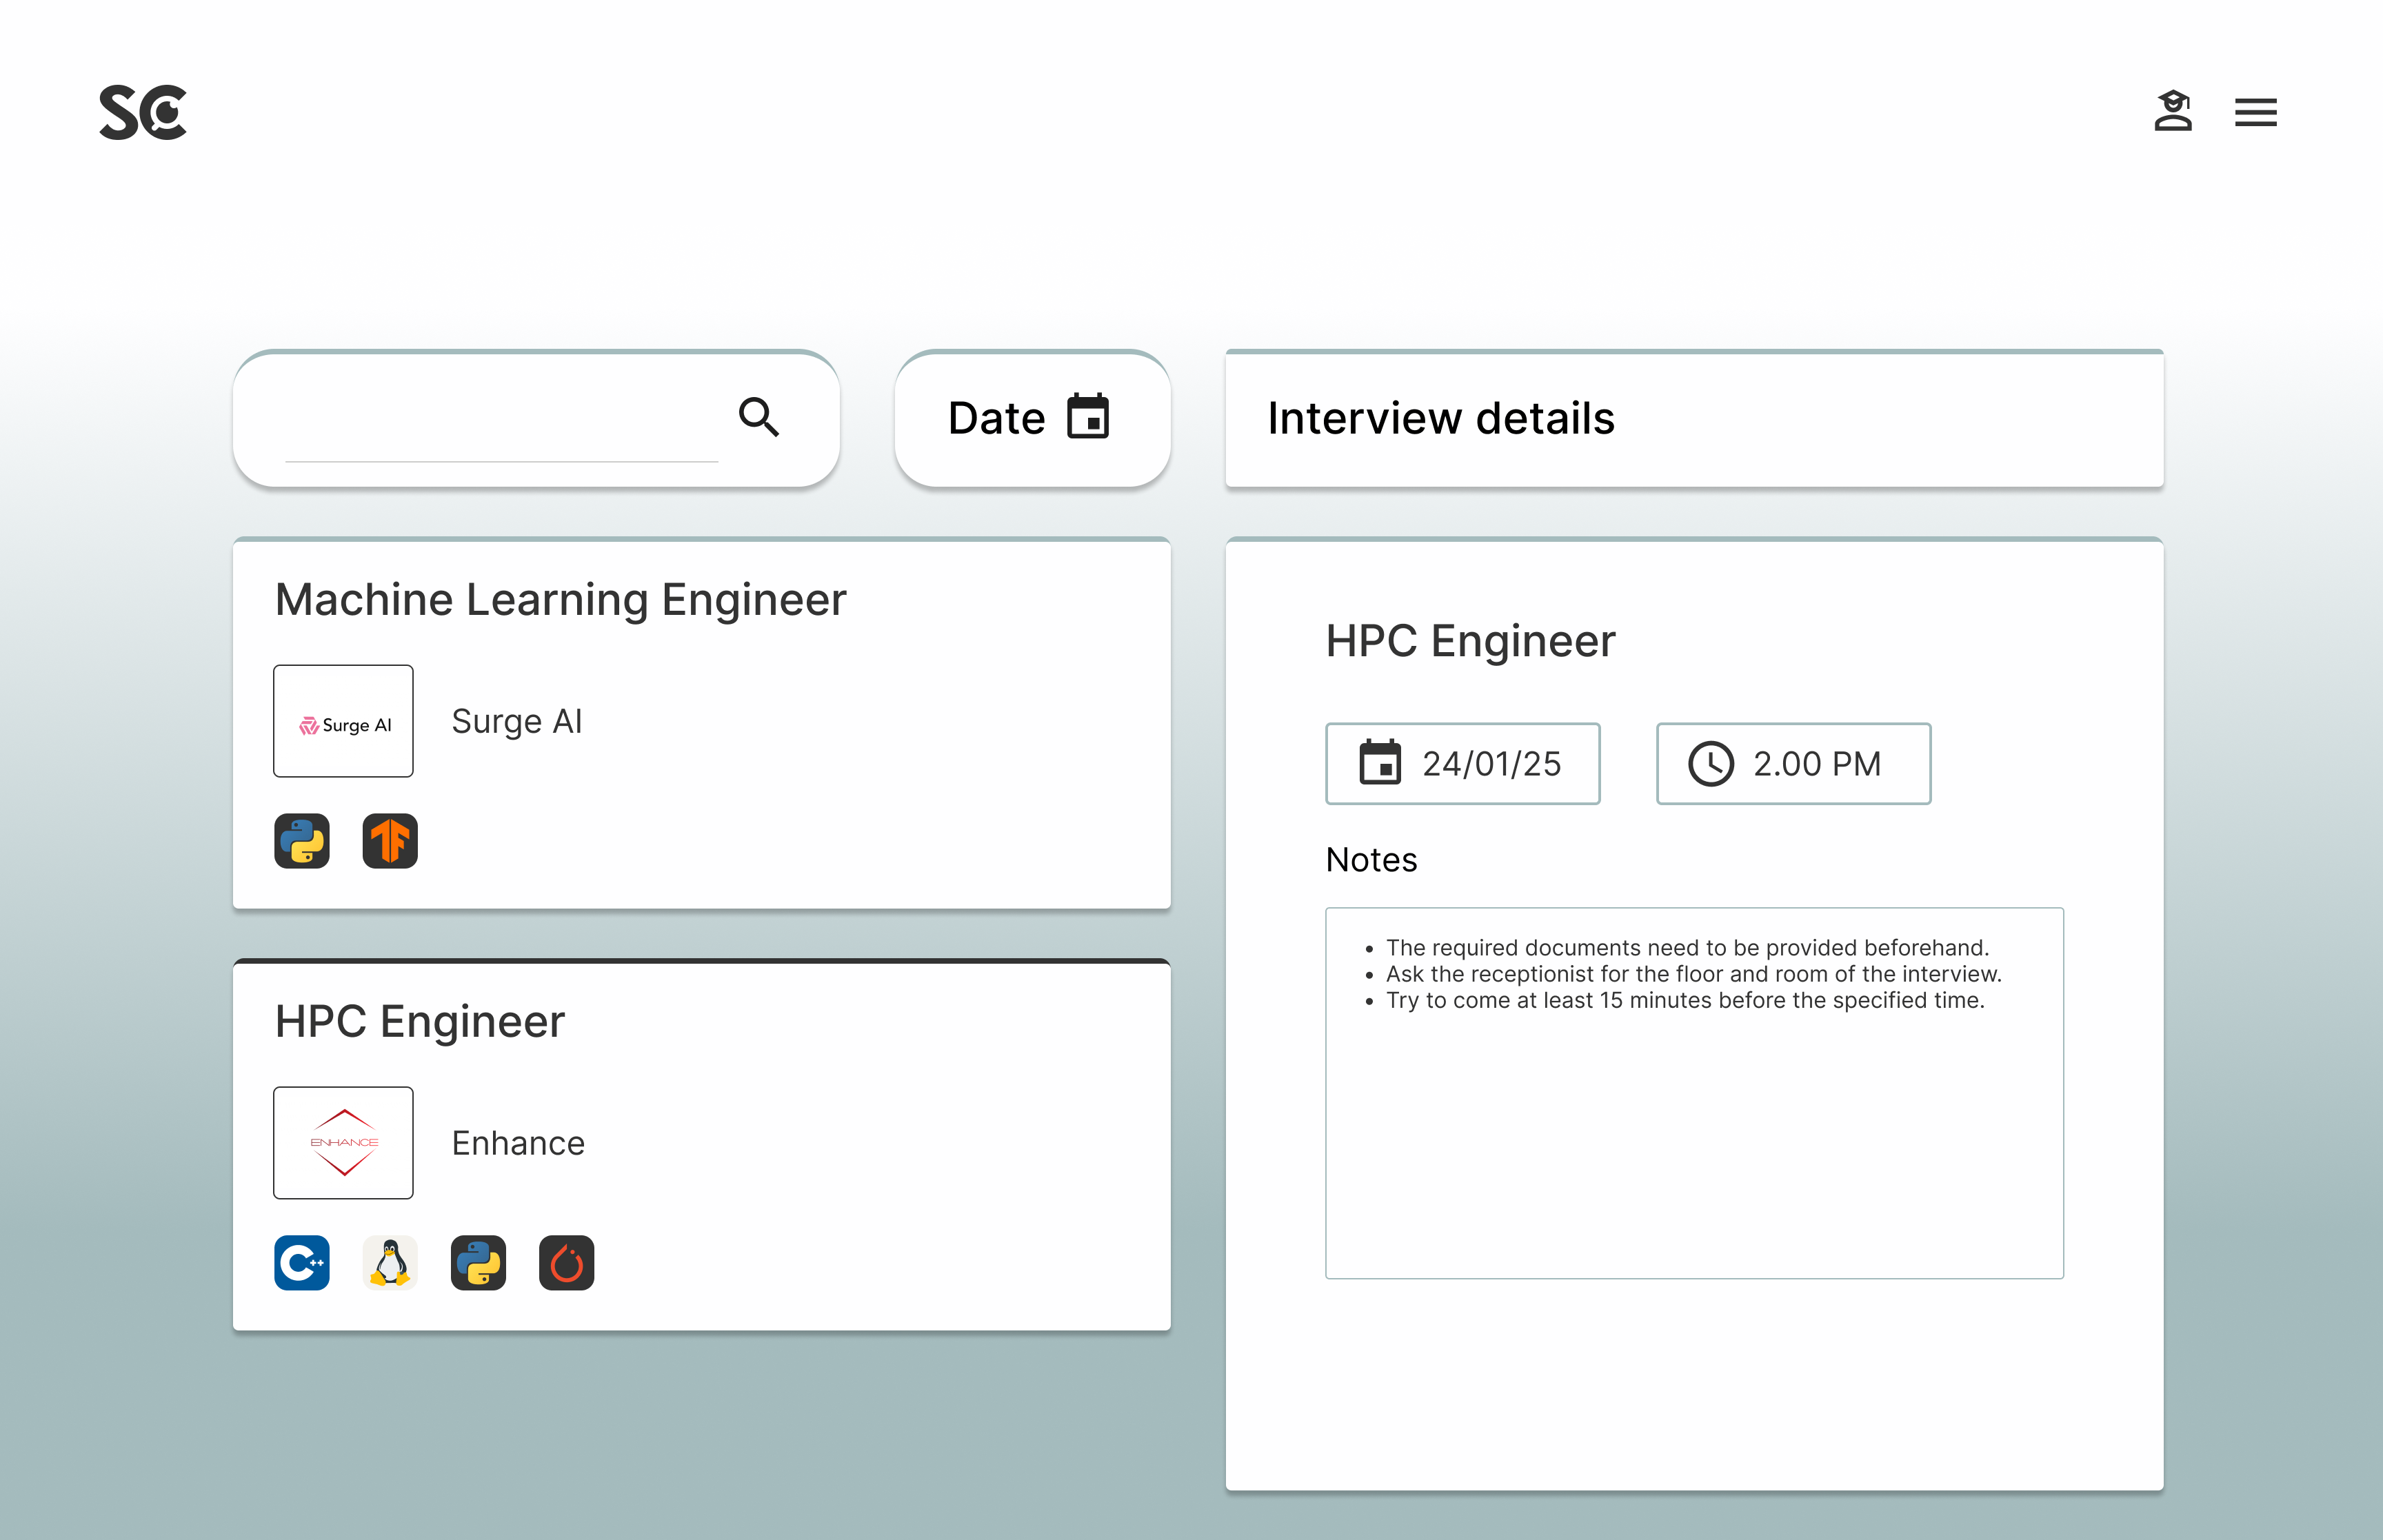
\includegraphics[width=0.8\textwidth]{Images/ui/View Planned interviews Student}
%    \caption{View Planned Interviews}
%    \label{fig:plannedIntStudent}
%\end{figure}
%
%Once we are done with the contact phase, and we are in the middle of the interview, if during the set up phase the Company added some questions, we will be presented with the following interface: a simple form, where we can see the proposed questions and we can simply answer them and submit once we are done.
%\begin{figure}[H]
%    \centering
%    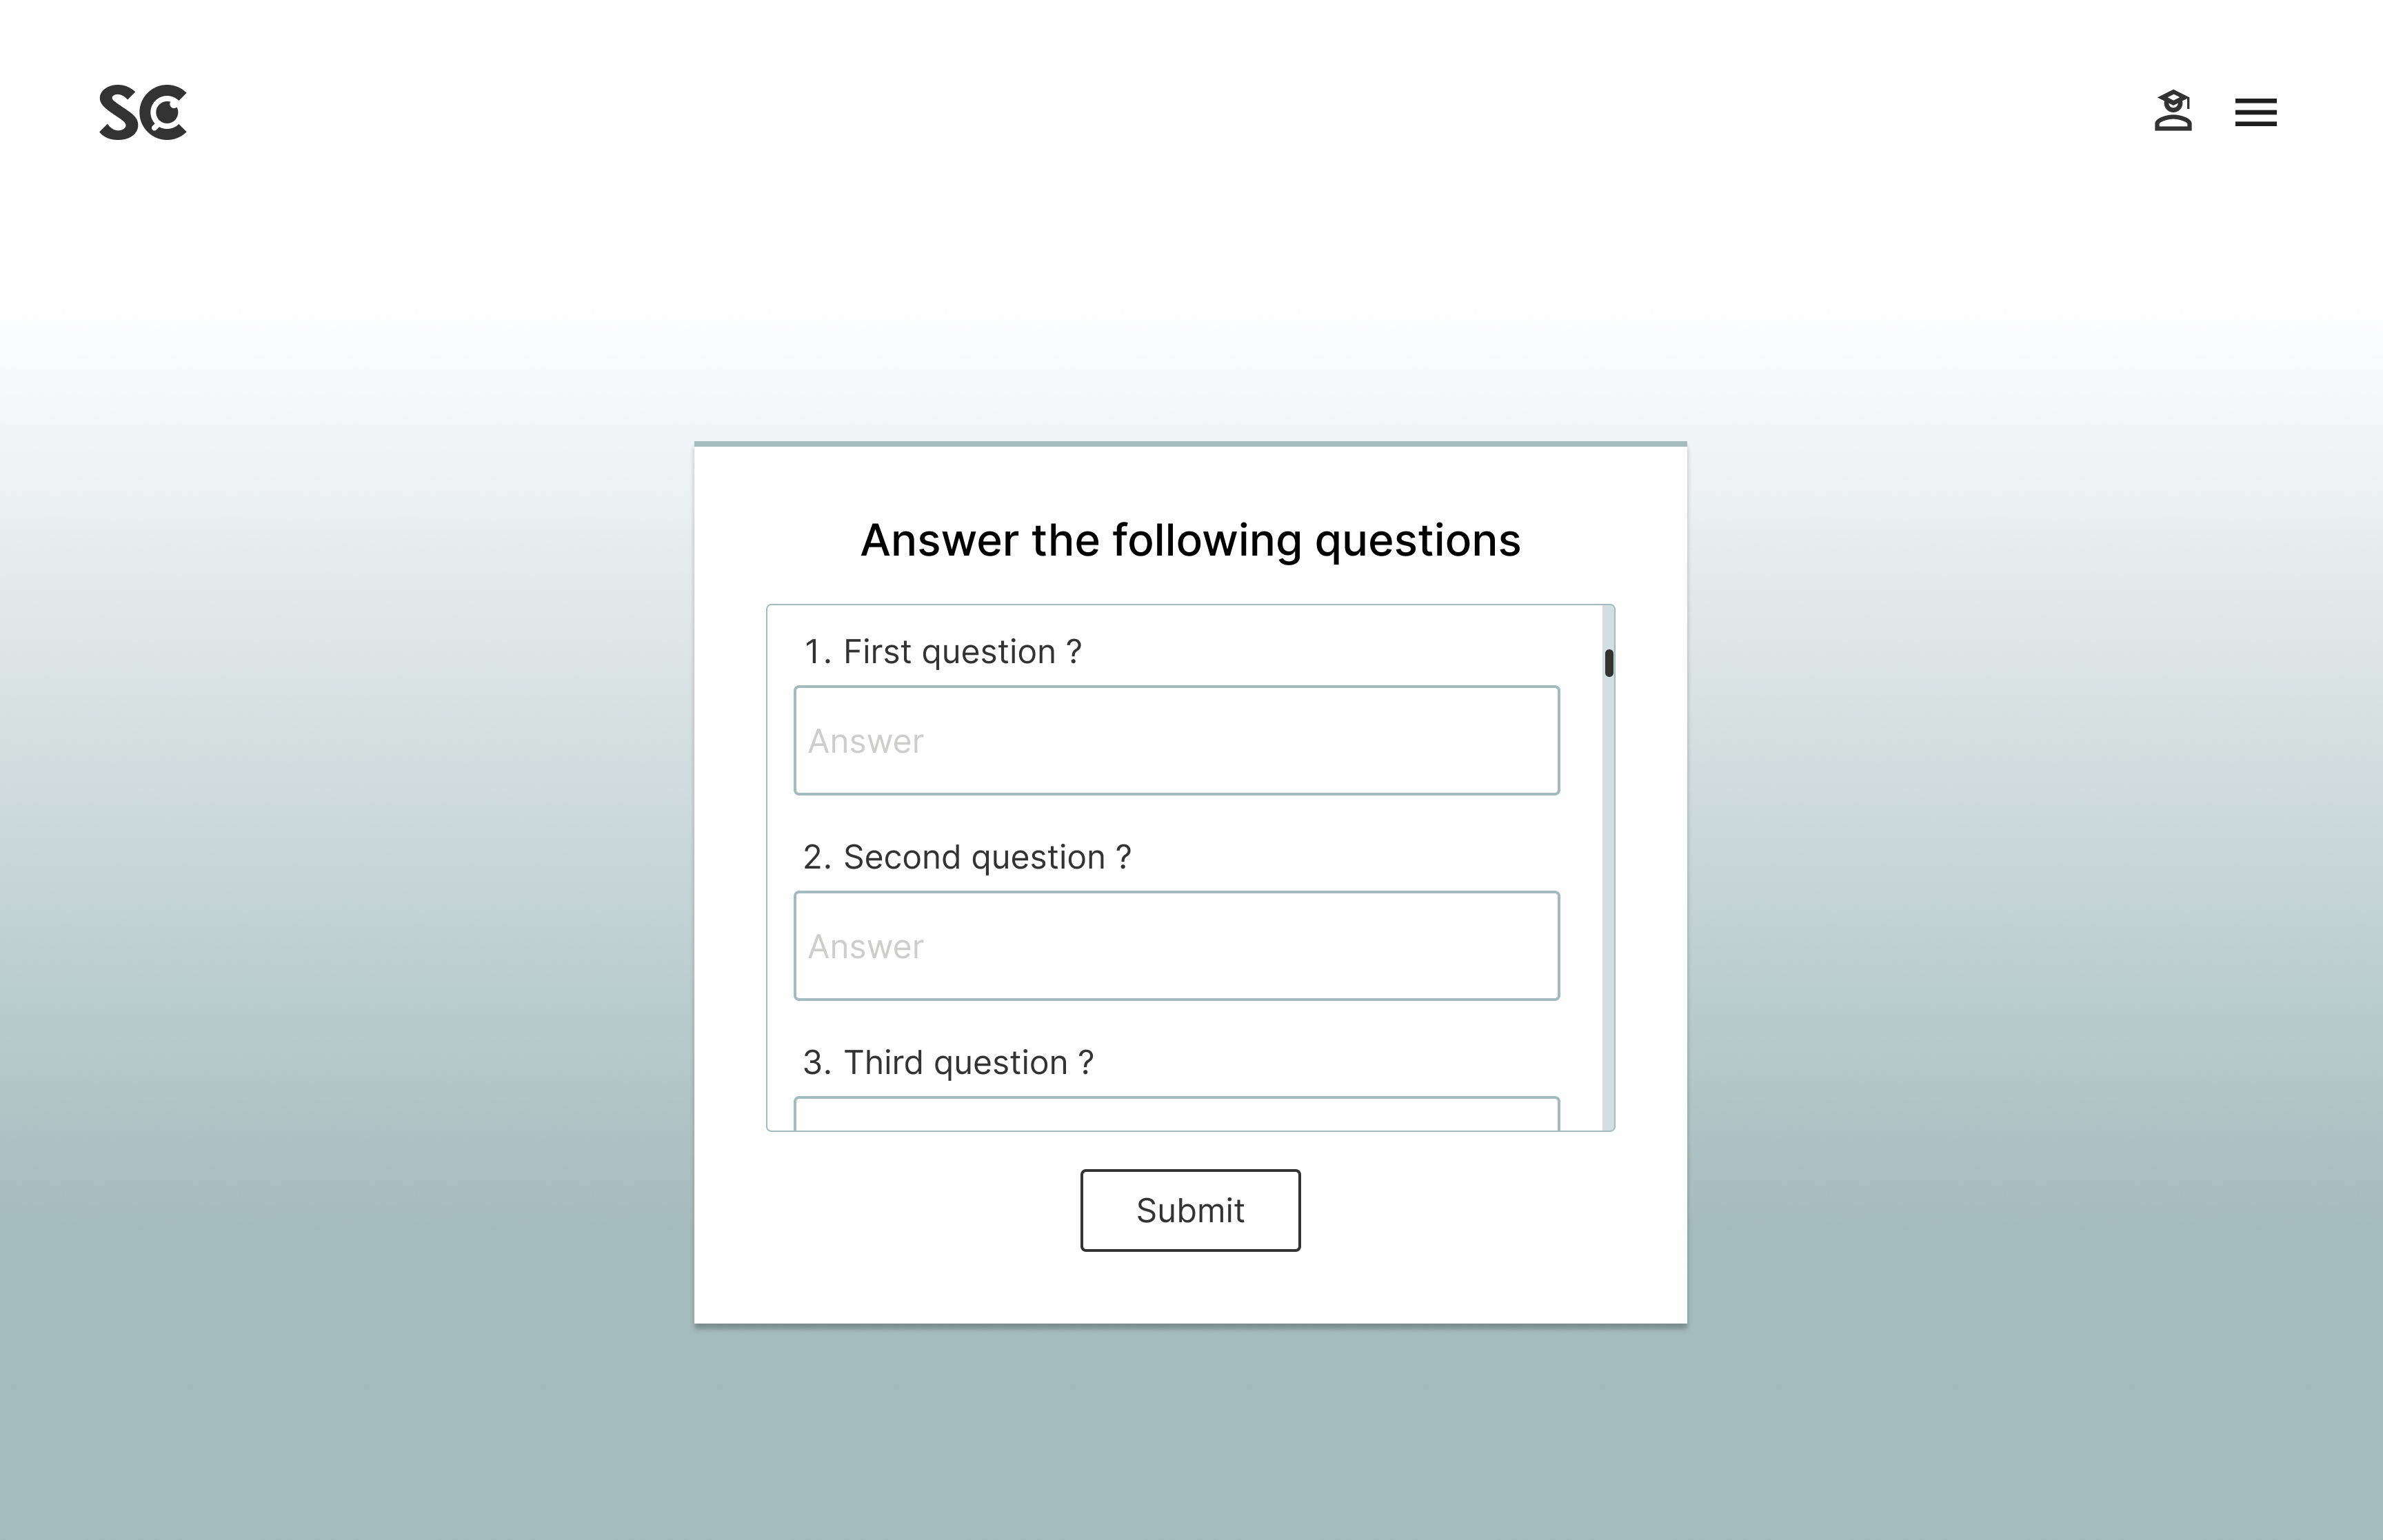
\includegraphics[width=0.8\textwidth]{Images/ui/Fill structured questioner}
%    \caption{Structured Questioner}
%    \label{fig:structuredQuestioner}
%\end{figure}
%
%To access all the previous interfaces we opted for a simple side menu, that can be accessed through the hamburger icon in the top right corner of the interface.
%Once the menu is opened, we can simply click on the desired functionality.
%\begin{figure}[H]
%    \centering
%    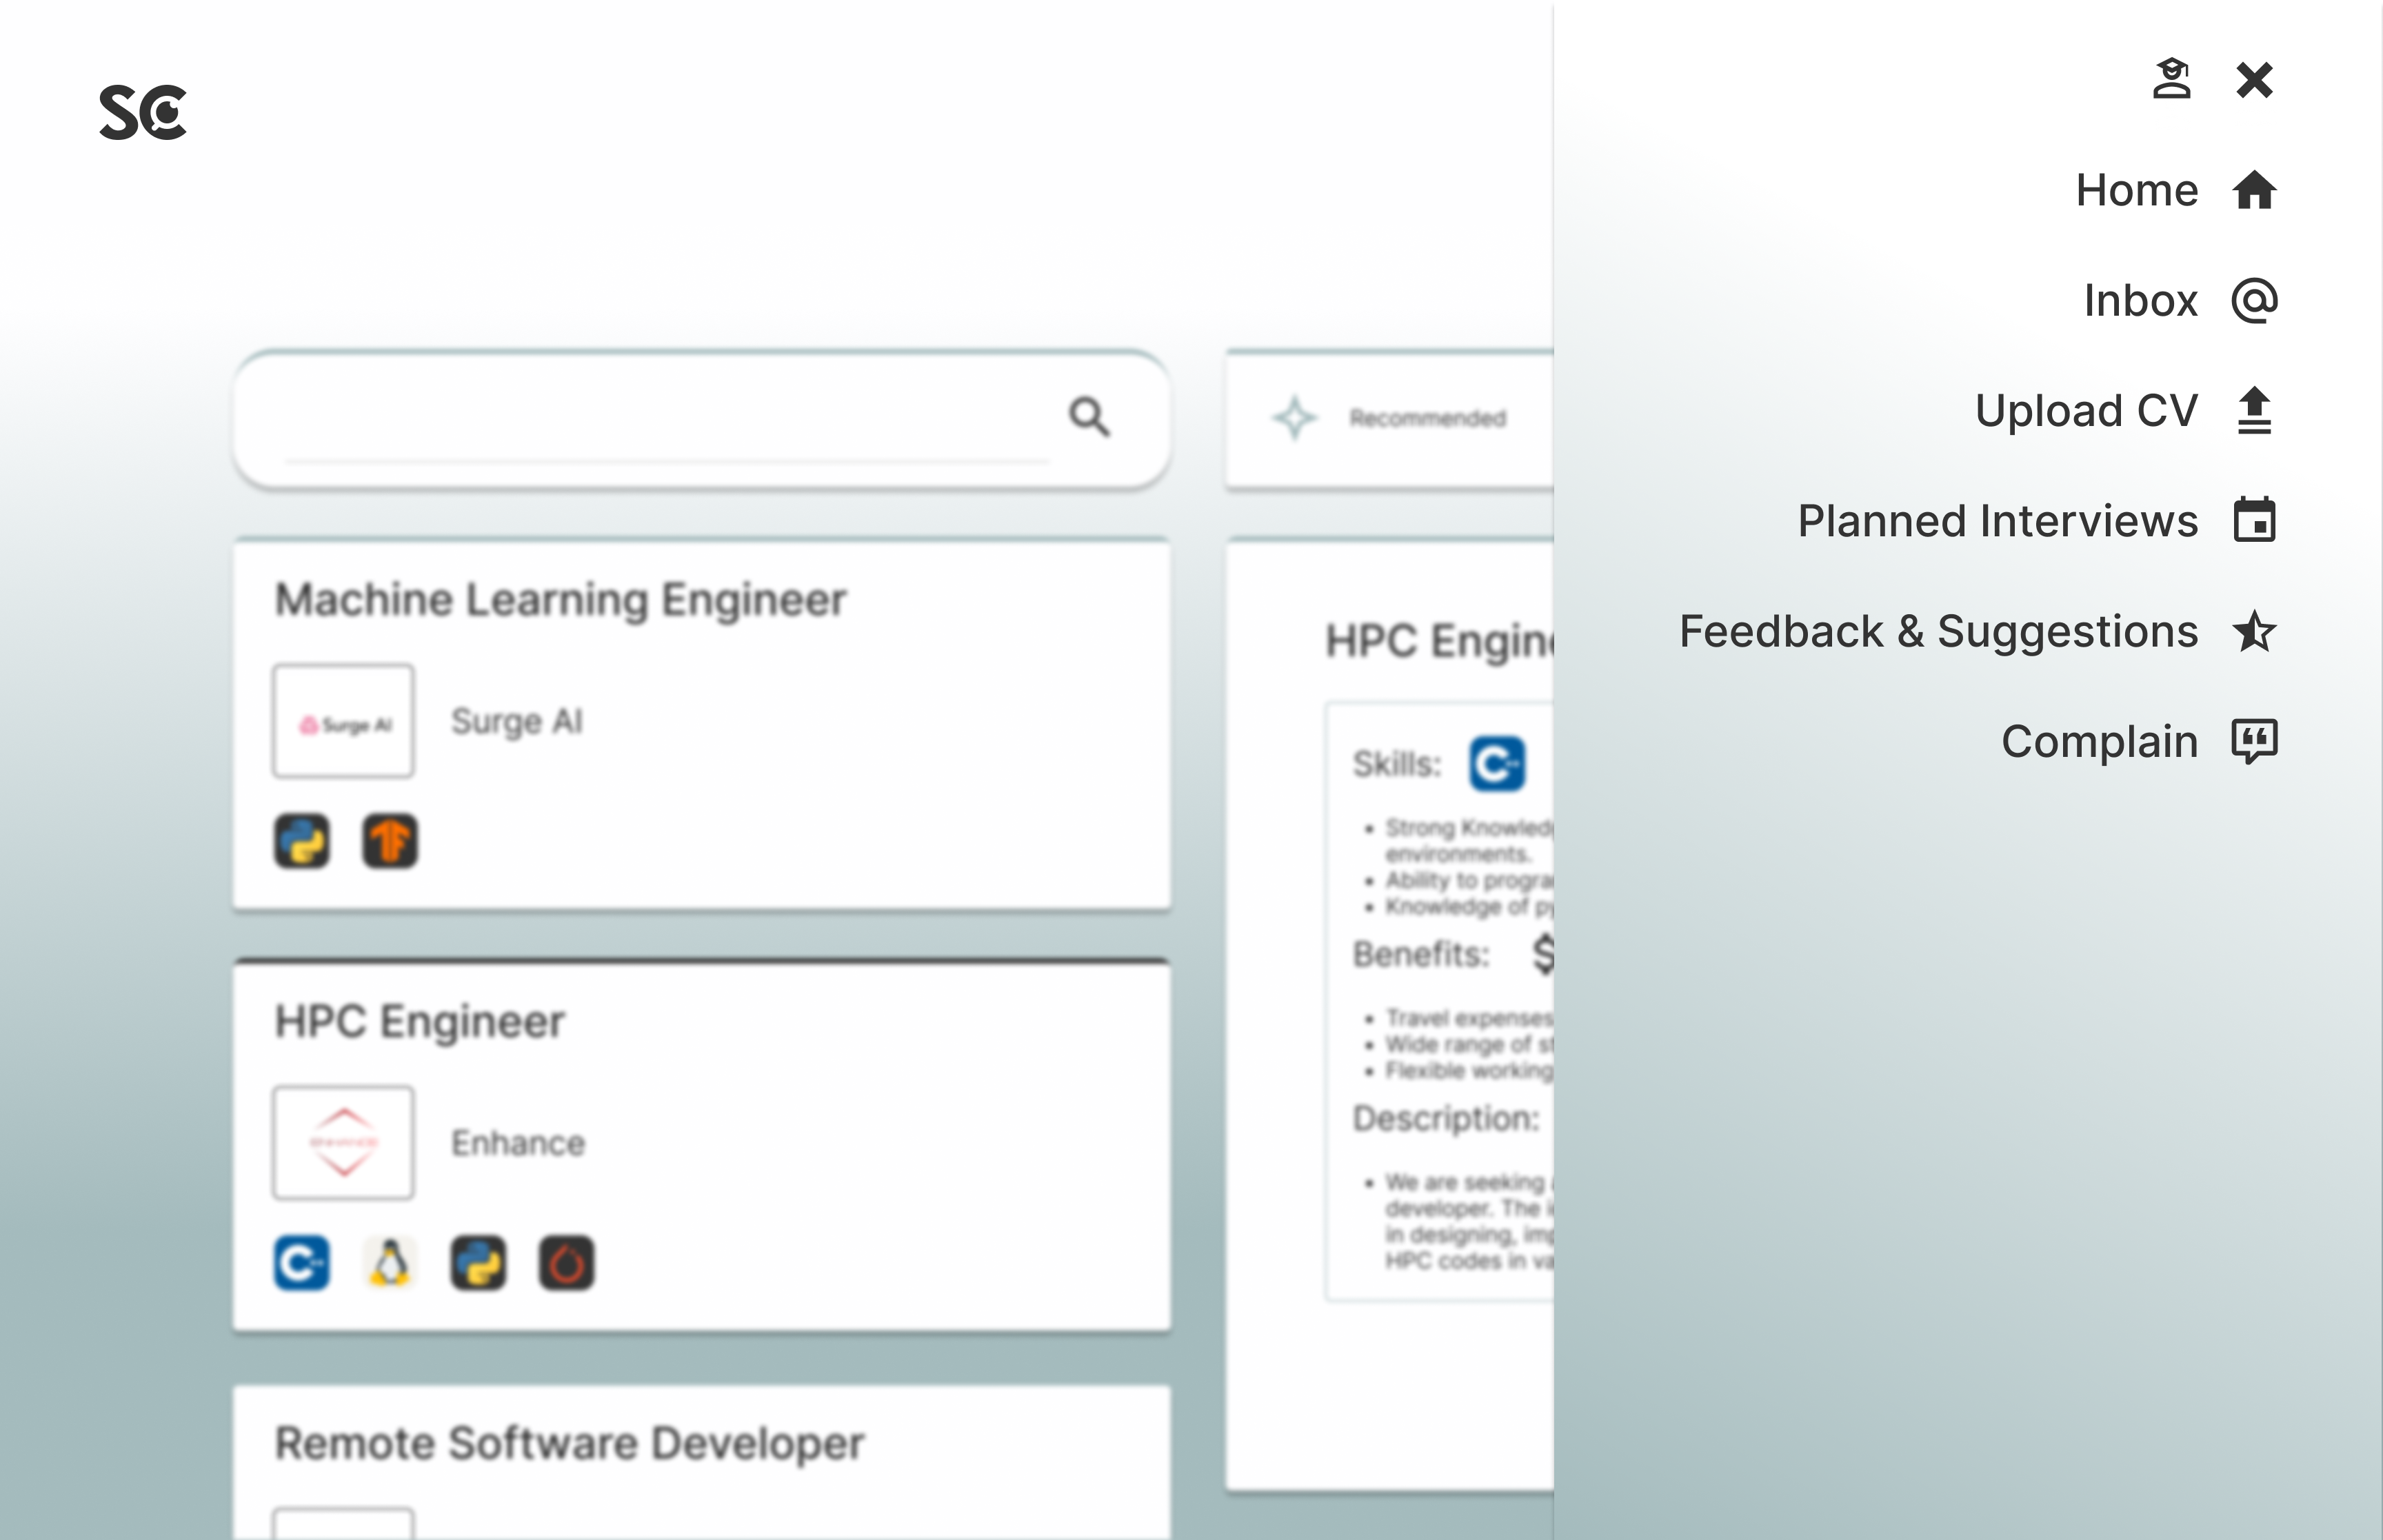
\includegraphics[width=0.8\textwidth]{Images/ui/Sidebar Student}
%    \caption{Student Menu}
%    \label{fig:studentMenu}
%\end{figure}
%
%
%\section{Company Interface}\label{sec:company-interface}
%Once a Company has logged in, the Published Internship page is shown, this is also the home page for a Company where we can find the list of all the published internships and information about them.
%The structure is simple:
%\begin{itemize}
%    \item On the left we have the list of the internships
%    \item The selected internship is denoted by the black accent on top of the item box
%    \item On the right, other than the details of the internship we have also two buttons, one used to view all the recommended students for the selected internship and the other to finalize the selection of the candidates that have been interviewed for that position.
%\end{itemize}
%\begin{figure}[H]
%    \centering
%    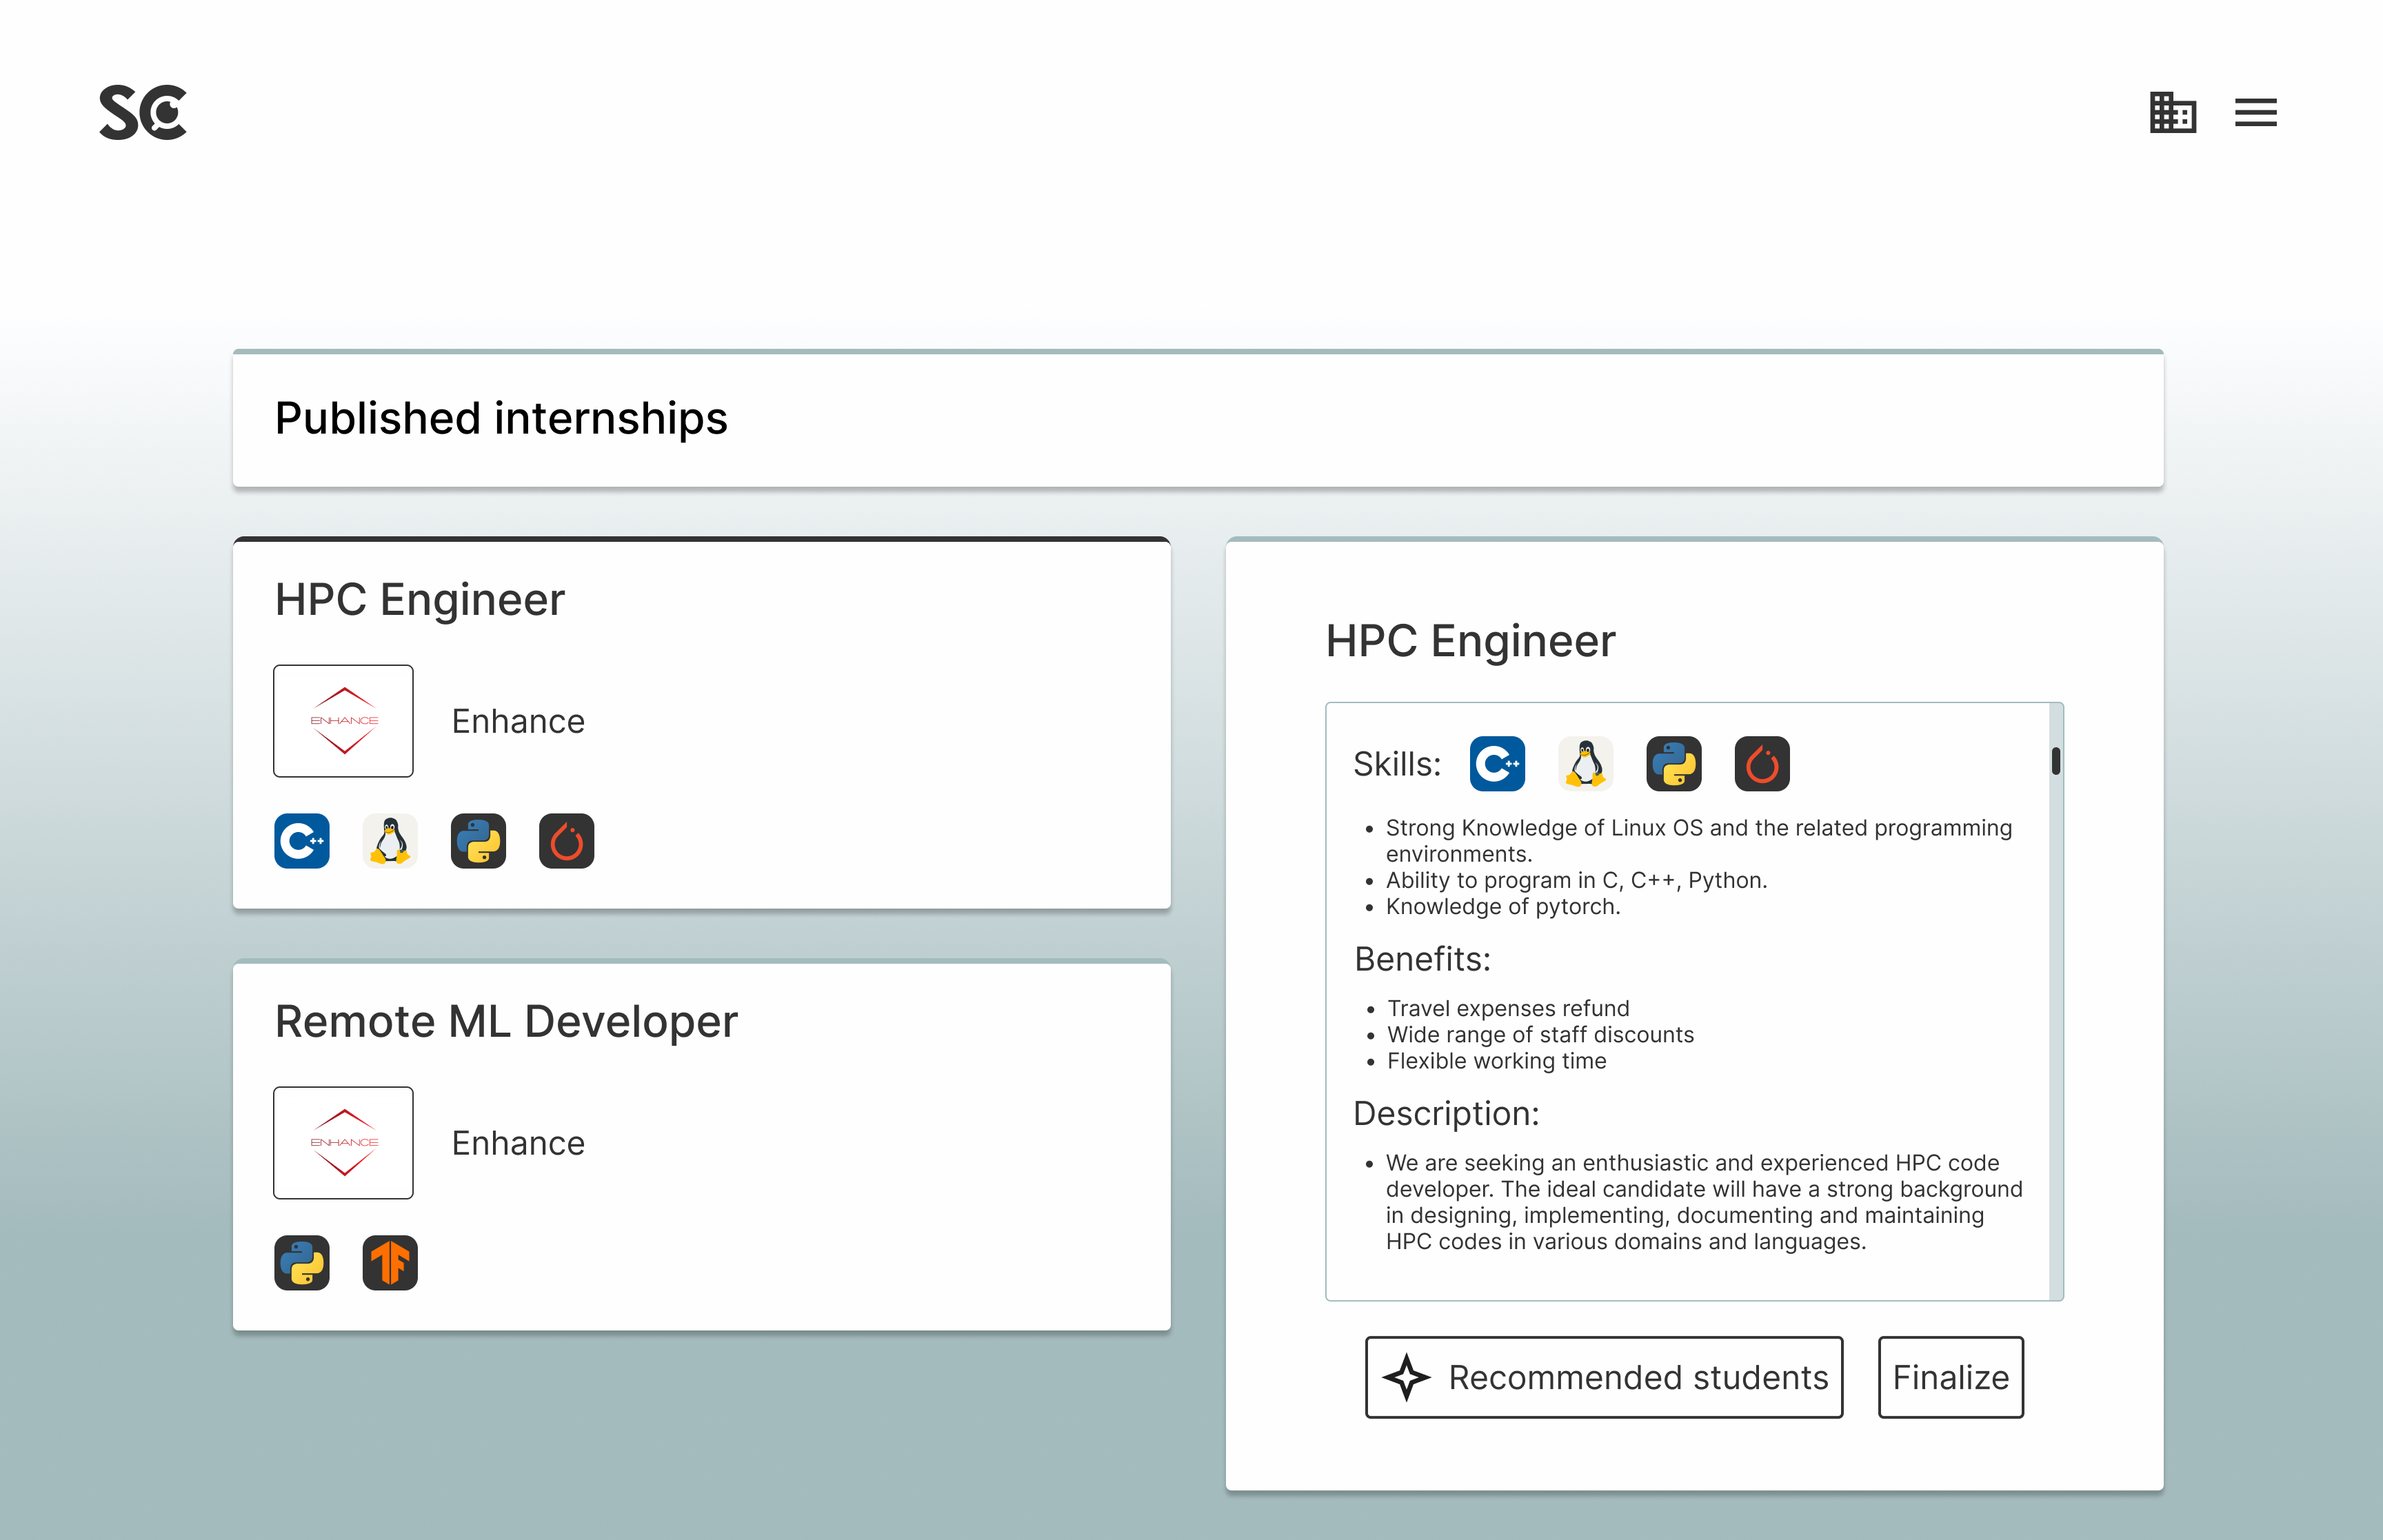
\includegraphics[width=0.8\textwidth]{Images/ui/View published internships}
%    \caption{View Published Interships}
%    \label{fig:publishedInternships}
%\end{figure}
%
%As mentioned before if we want to see the recommended students for a selected internship we simply need to click on the corresponding button, and we will be redirected to the View Recommended Students page.
%Here we can see:
%\begin{itemize}
%    \item On the left the list of all the recommended students, that we can filter by using the appropriate searchbar.
%    \item In the list we can see a few basic information, such as the name of the student as well as his university.
%    \item On the top right we can see the name of the internship for which we view the recommended students
%    \item On the right we can also see the details of the selected student, with his resume.
%    \item In the same detail section we can also use a button to send an offer for that internship.
%\end{itemize}
%\begin{figure}[H]
%    \centering
%    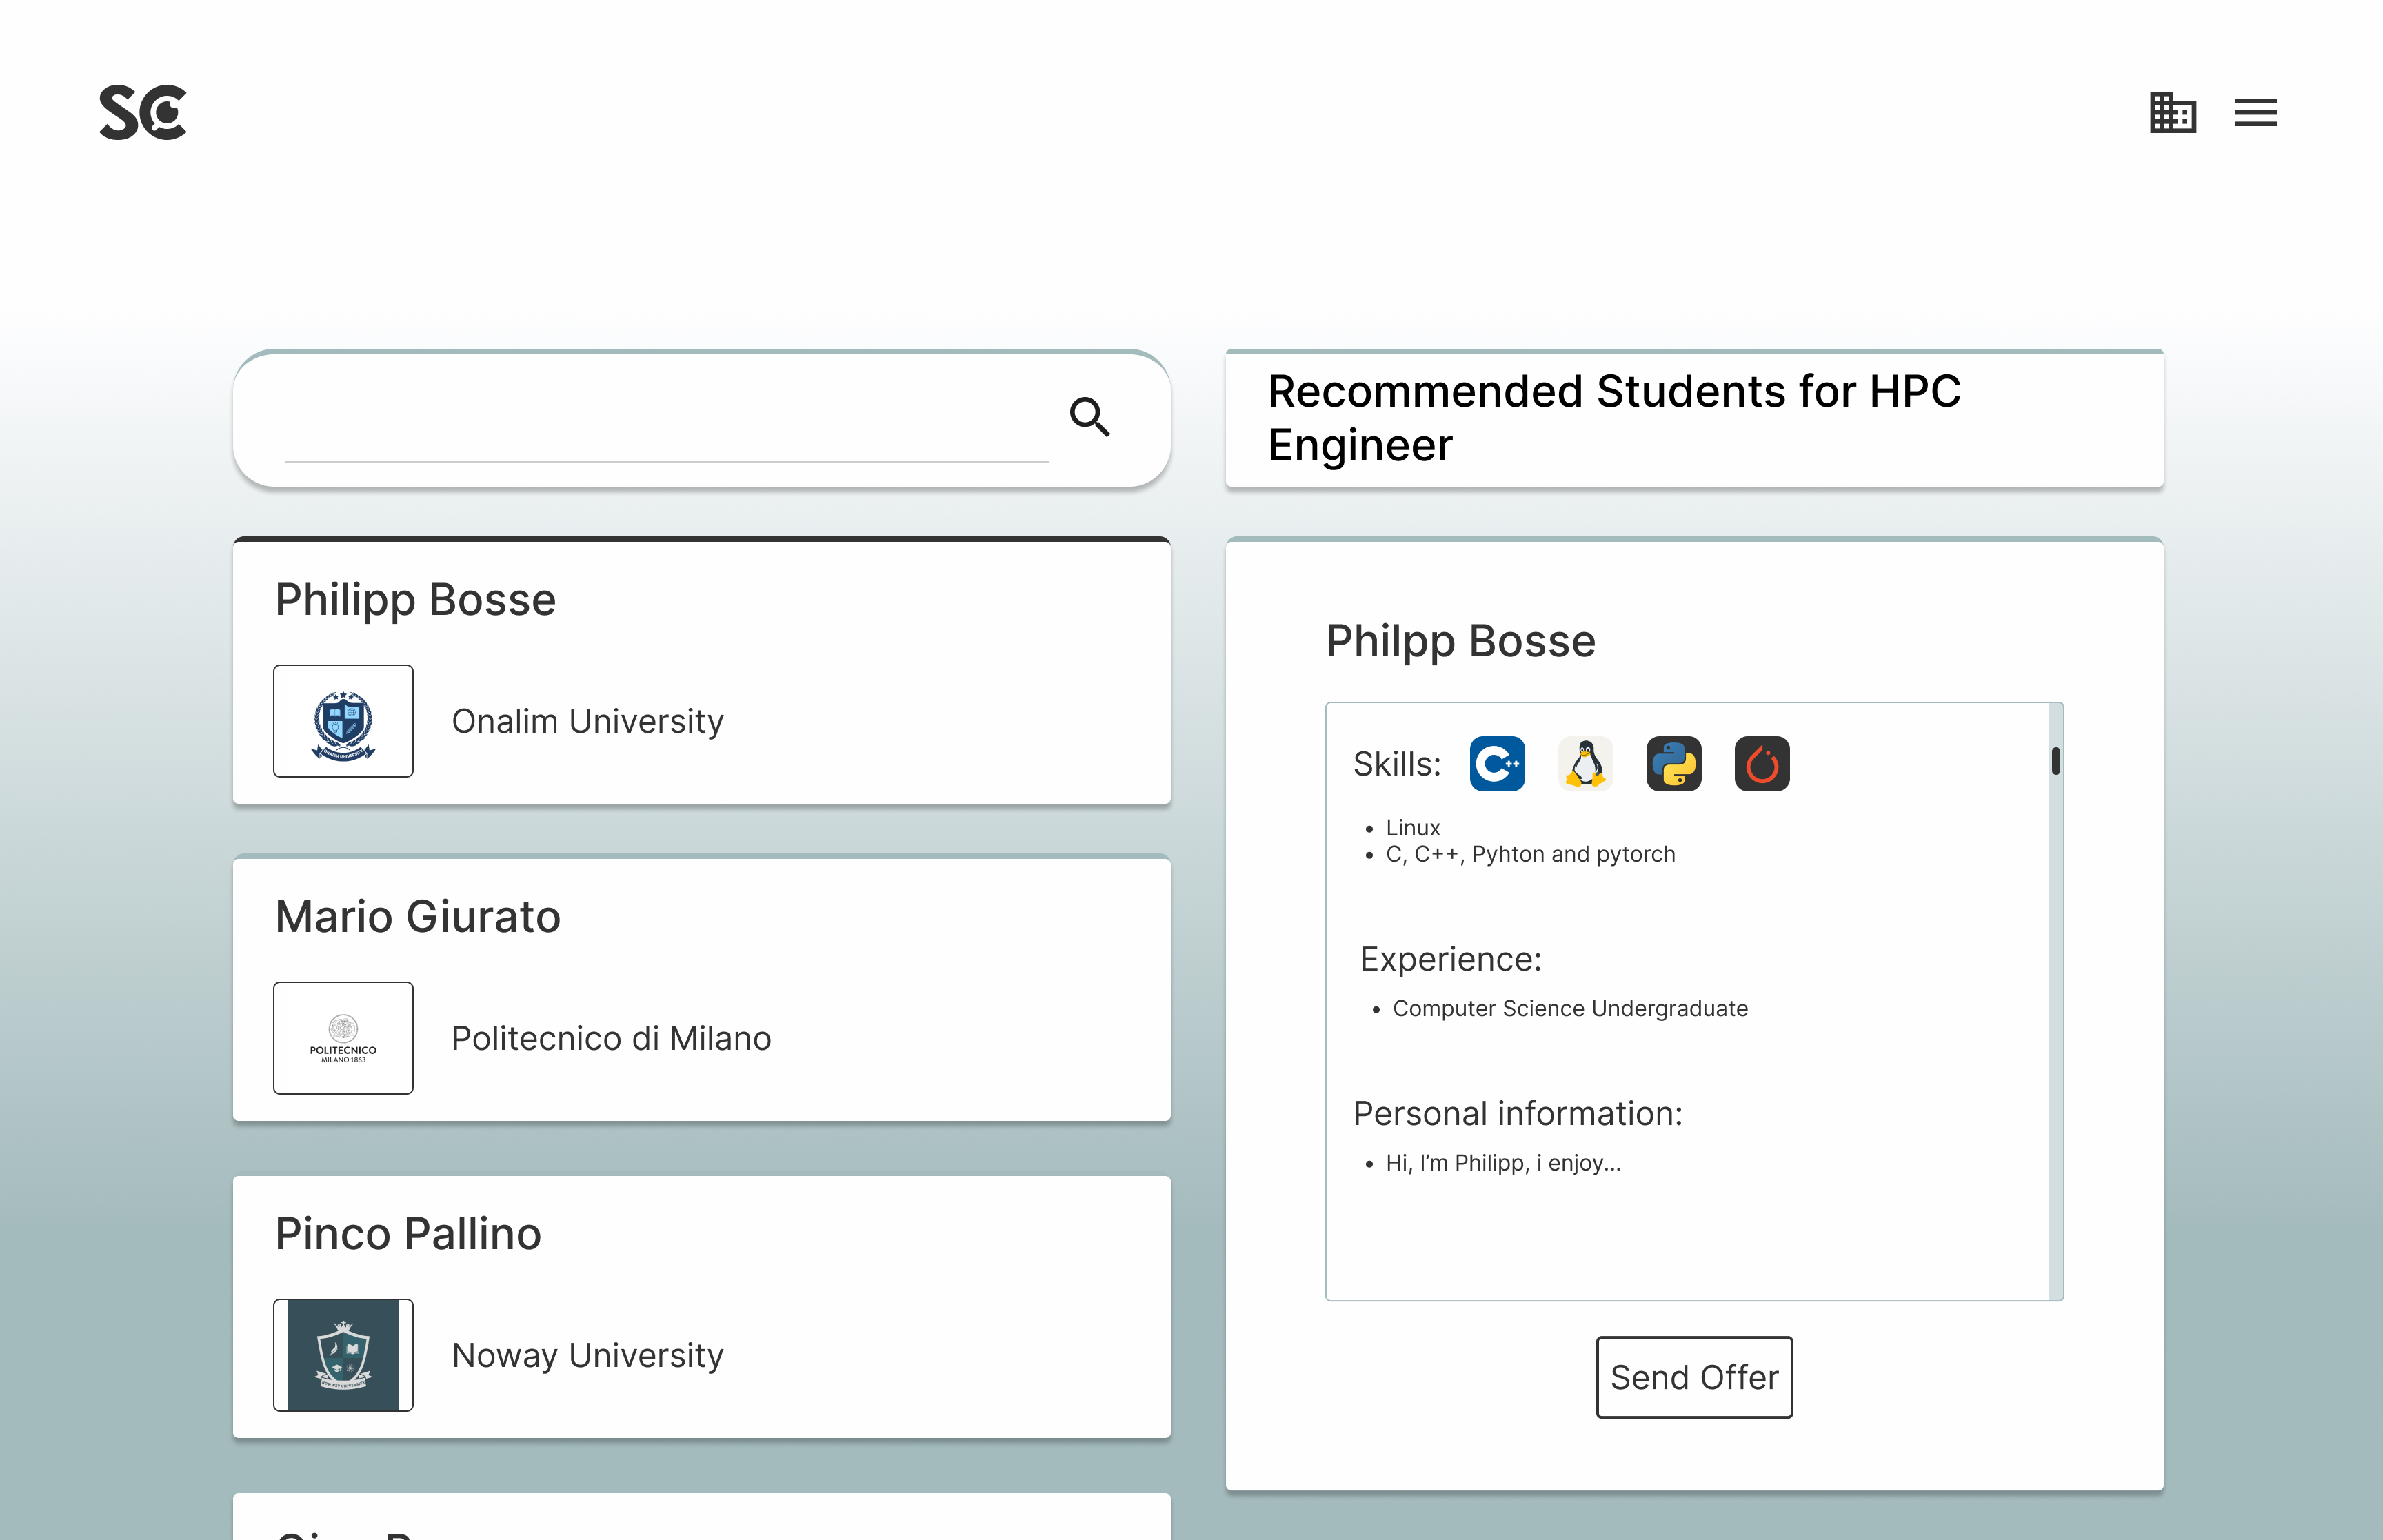
\includegraphics[width=0.8\textwidth]{Images/ui/View Recommended Students}
%    \caption{View Recommended Students }
%    \label{fig:recommendedStudents}
%\end{figure}
%
%Another core functionality is the ability to publish an internship.
%This can be done in the Publish Internship page, where we can fill a form with a title, the skills required, the description and the benefits for the position offered.
%To publish the internship simply click on the Publish button at the bottom of the form.
%\begin{figure}[H]
%    \centering
%    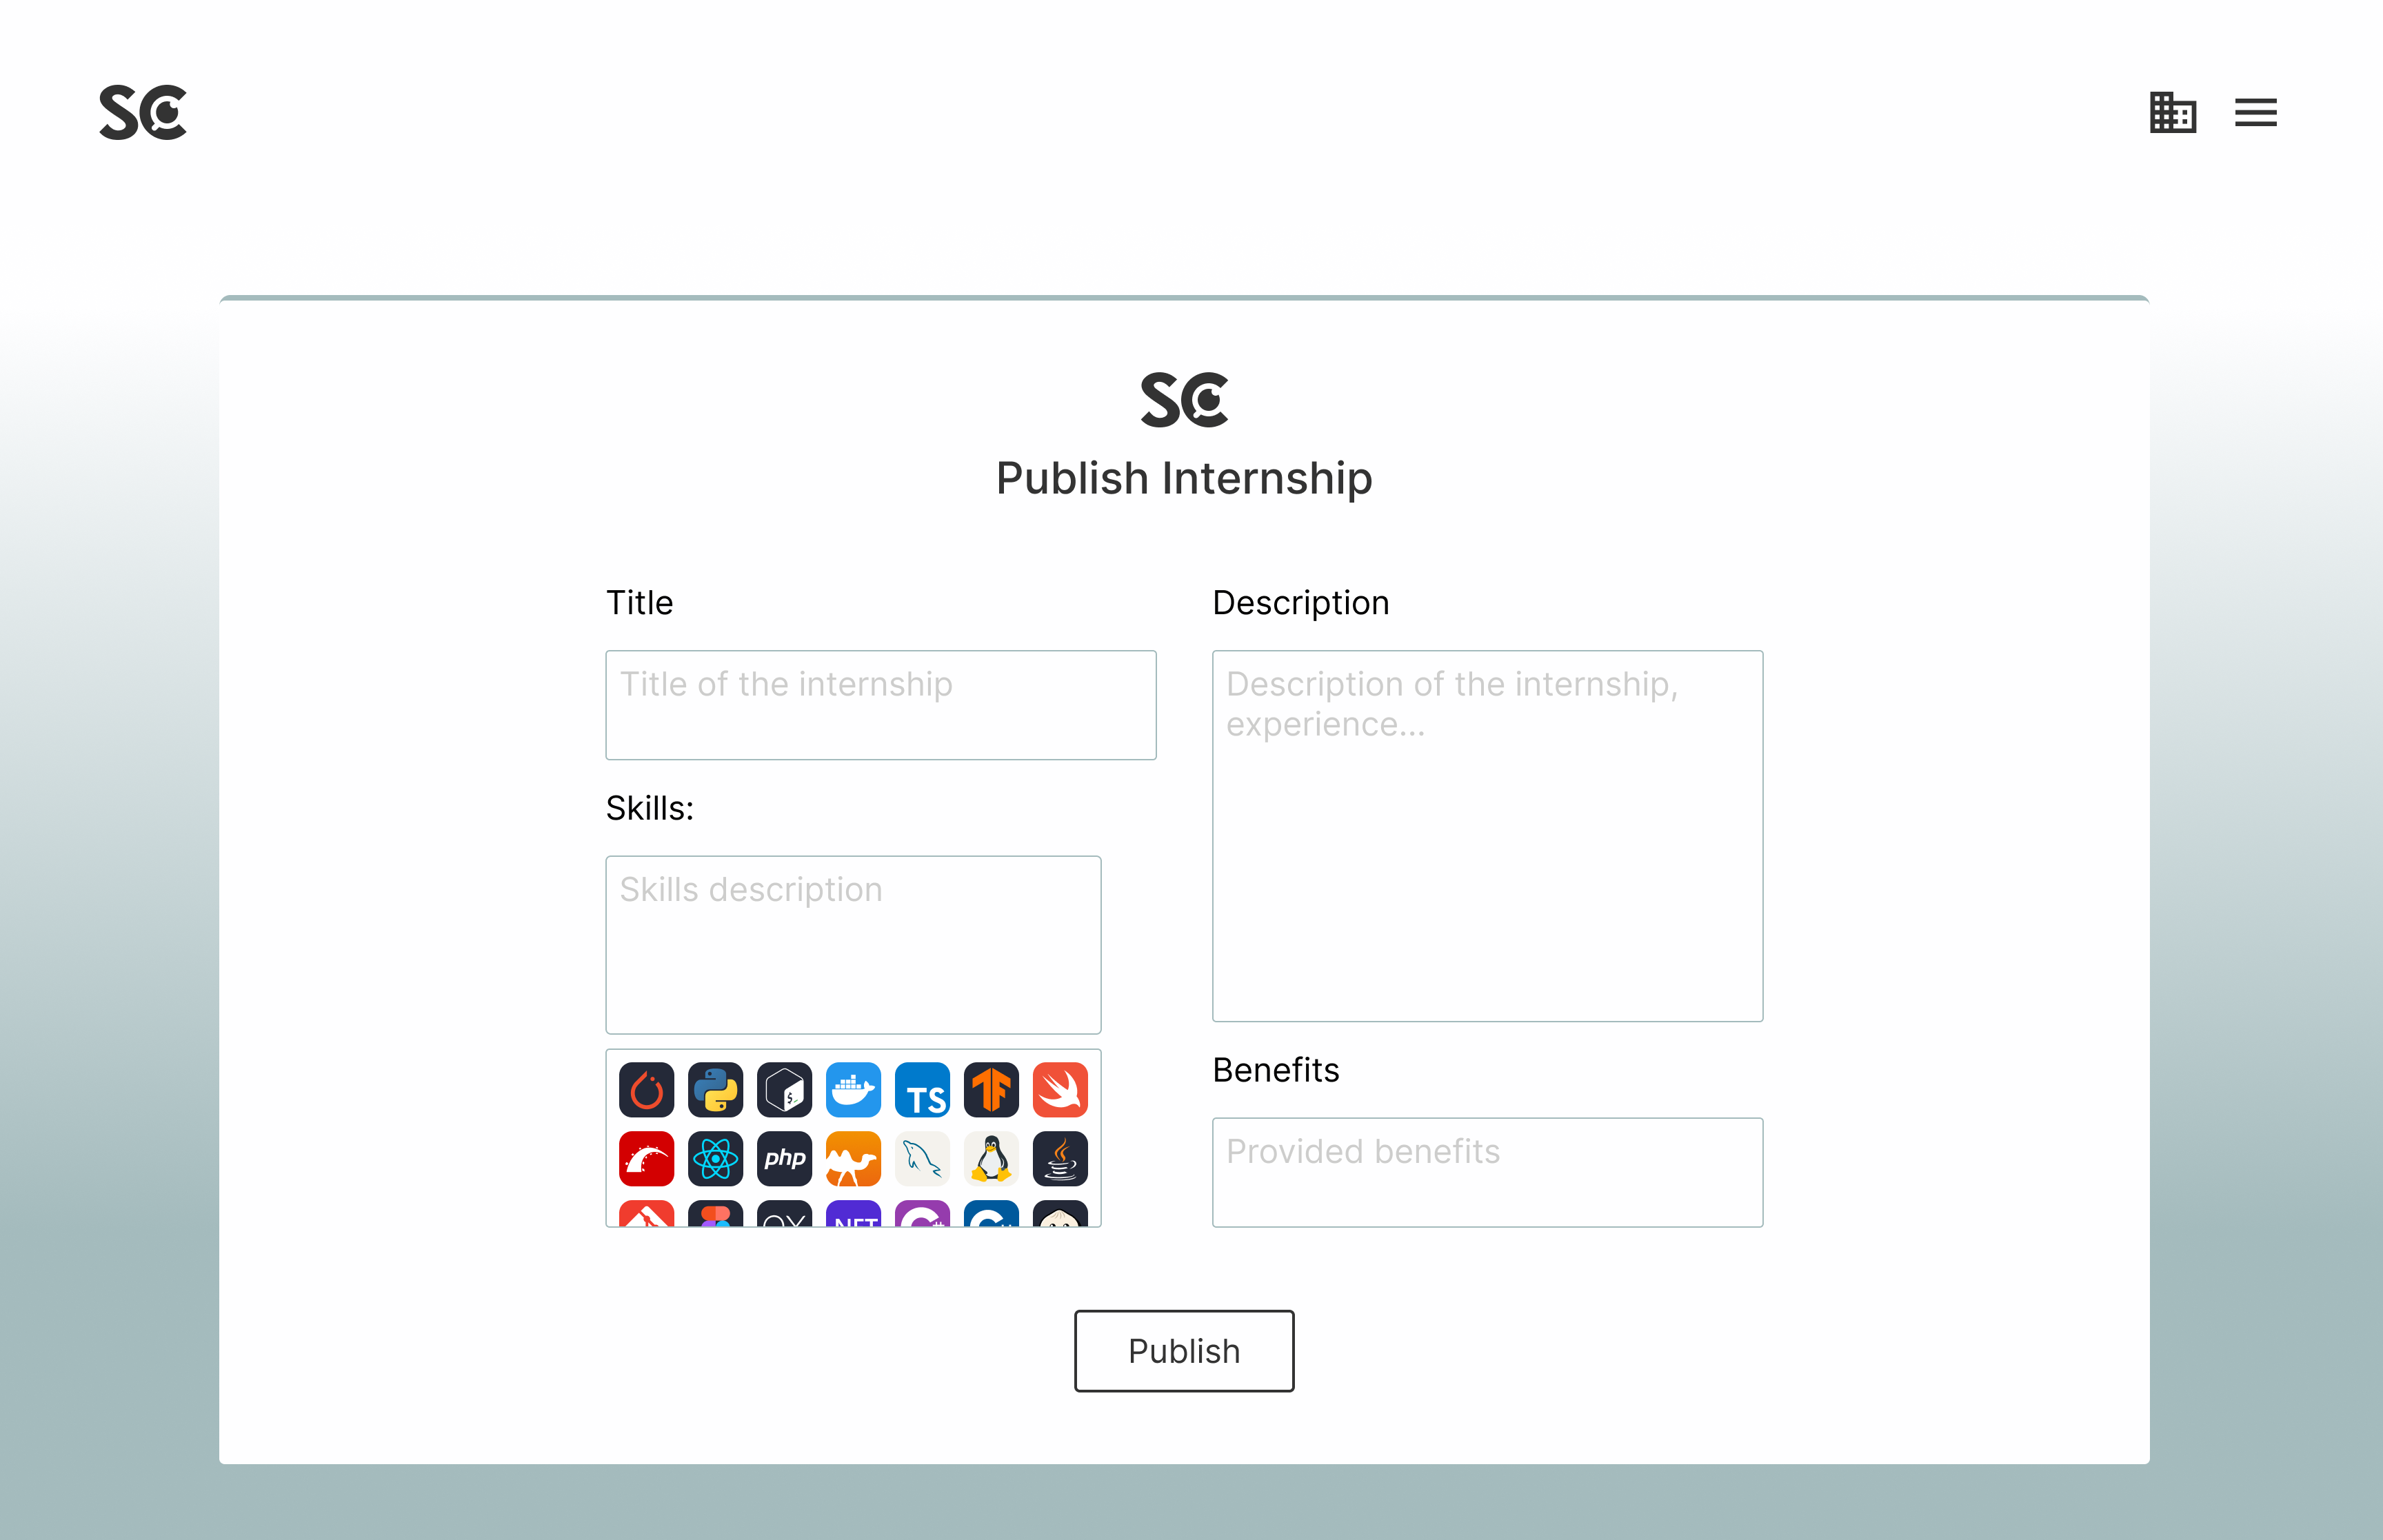
\includegraphics[width=0.8\textwidth]{Images/ui/Publish Internship}
%    \caption{Publish Internship}
%    \label{fig:pubIntenrship}
%\end{figure}
%
%Similarly to the Student interface, we also have an inbox, where we can find and mange all the notifications.
%In this case we could have an application for an open position, and we can decide to either accept or reject it in the same way the student did with offers.
%\begin{figure}[H]
%    \centering
%    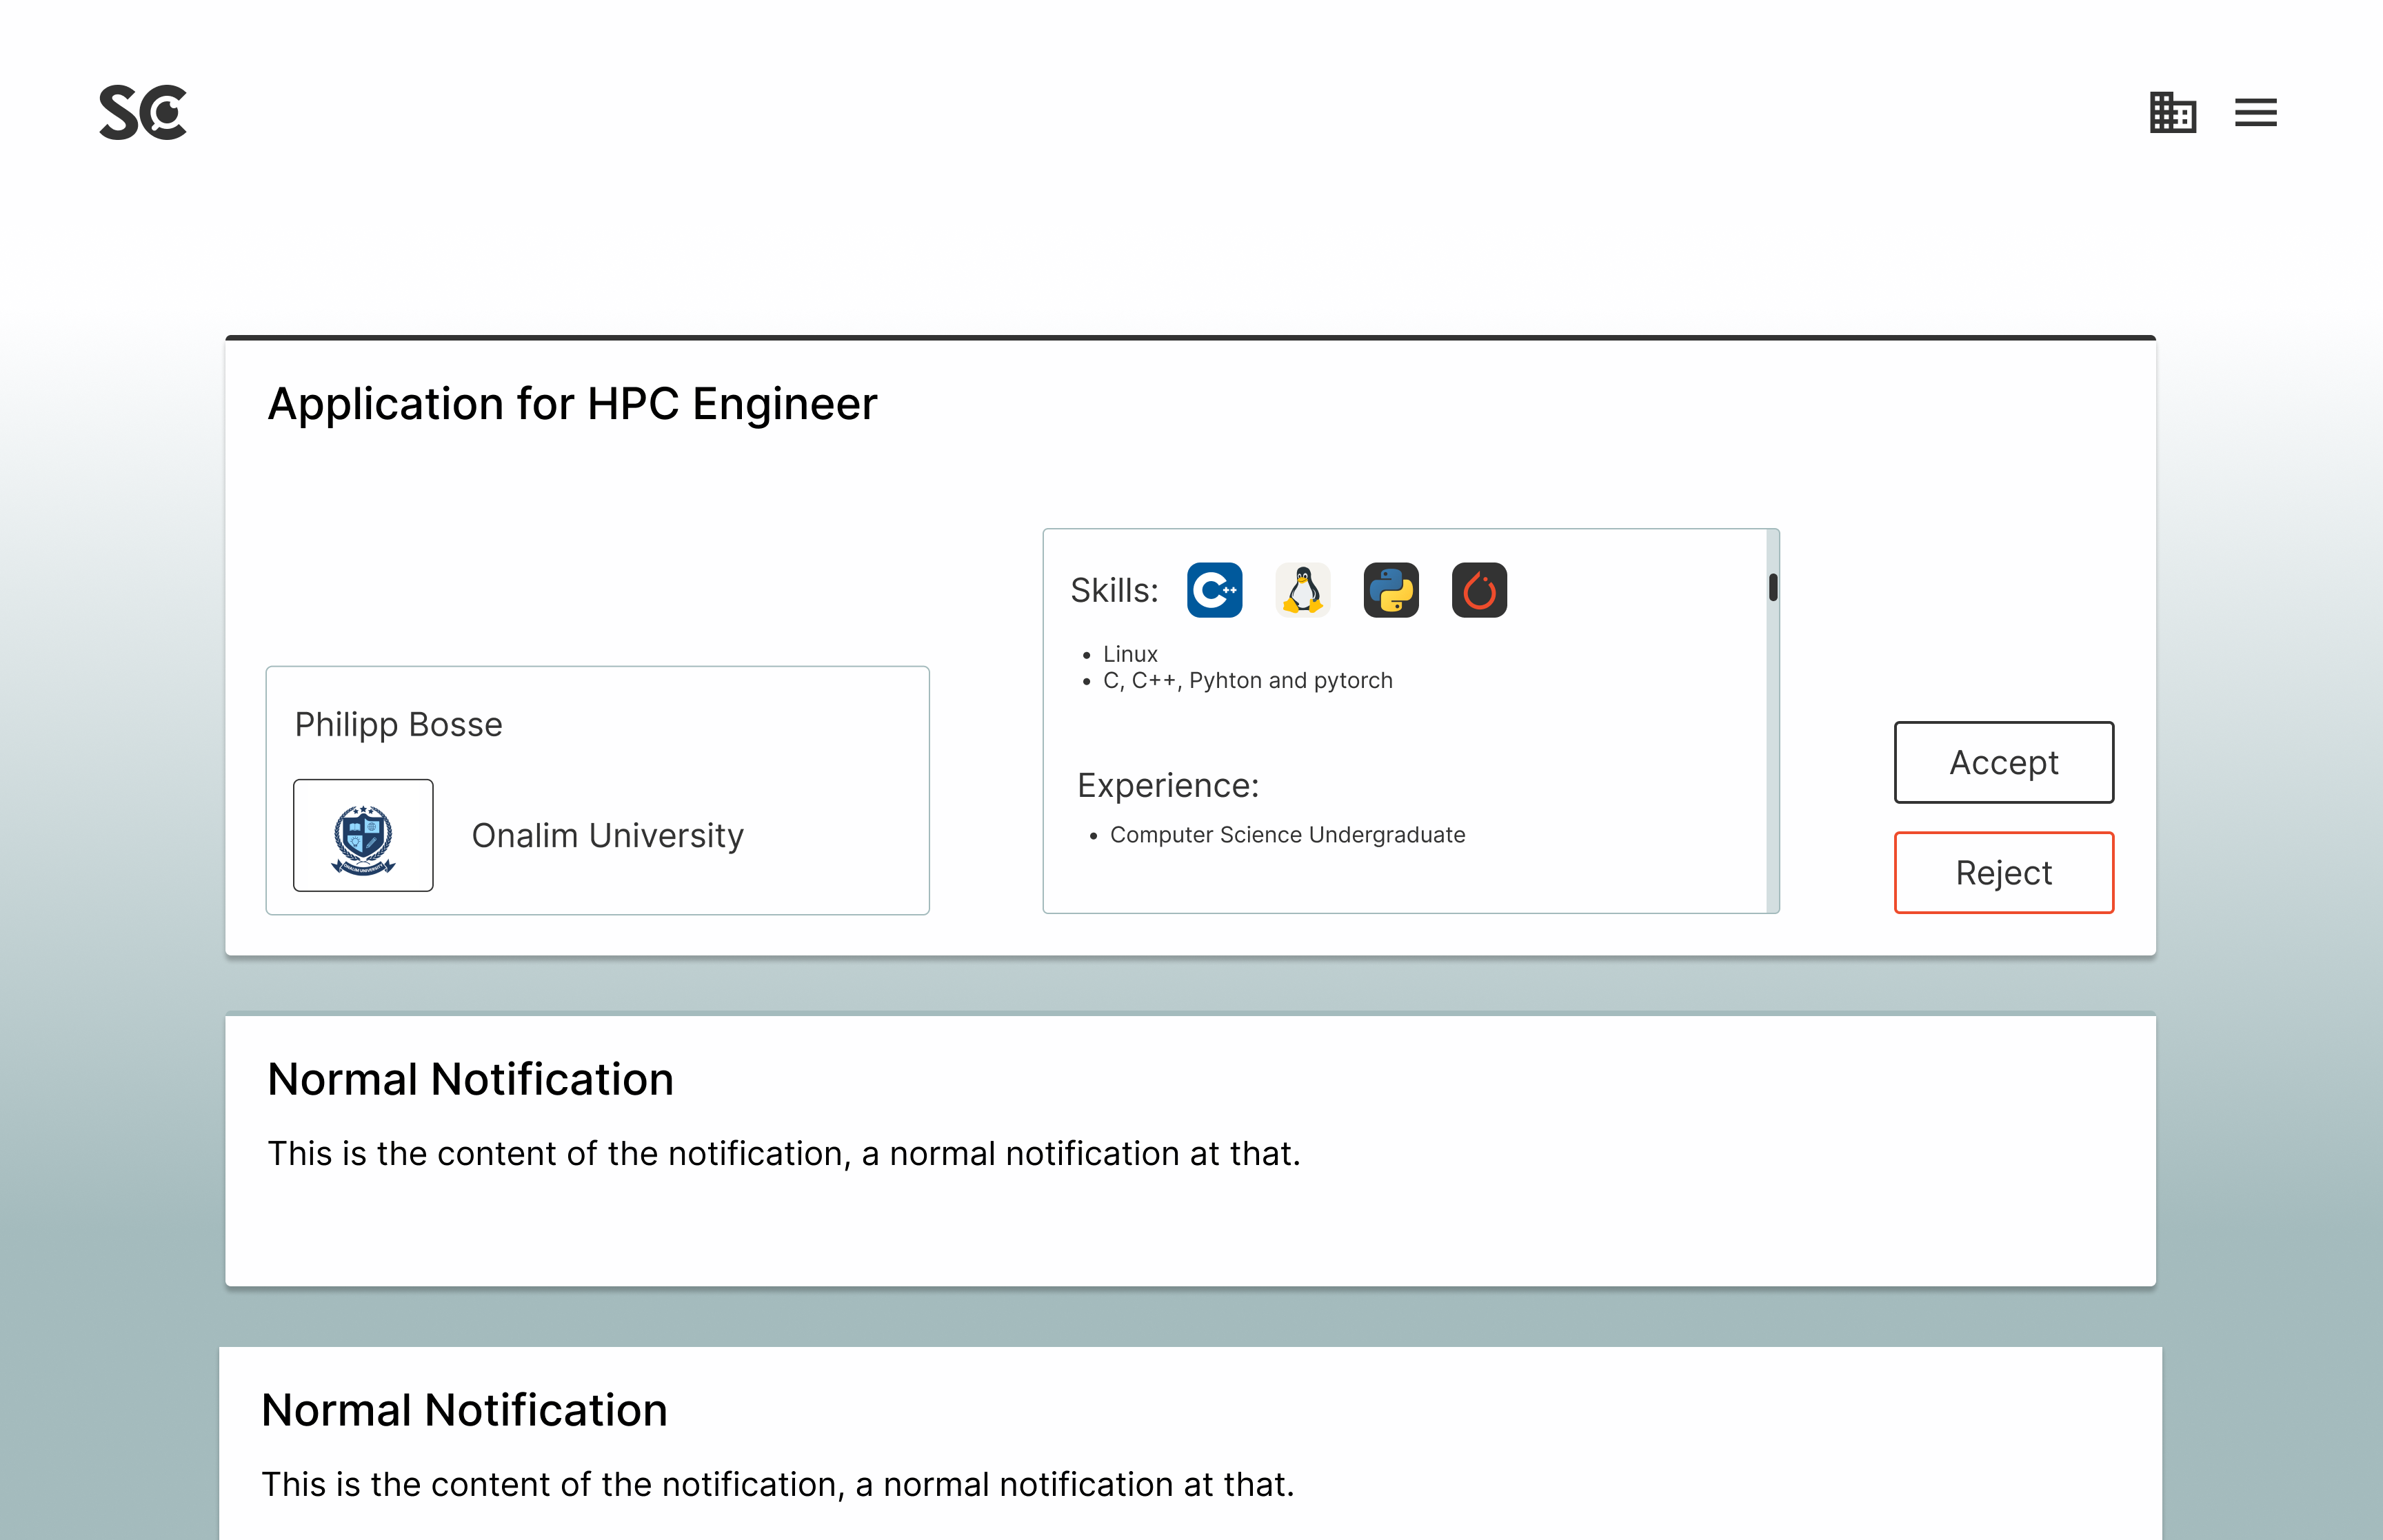
\includegraphics[width=0.8\textwidth]{Images/ui/Consider Application}
%    \caption{Company Inbox}
%    \label{fig:companyInbox}
%\end{figure}
%
%% TODO: need to add question for structured questioner here...
%Another important aspect is Setting Up interviews after finding a good candidate.
%This can be done with the Setup Interview page, where we can select via the dropdown menus on the left the candidate, date and time for the interview.
%On the right there is also the space to complete with some additional notes.
%In this section we also add the questions that will be part of the structured questioner during the interview.
%\begin{figure}[H]
%    \centering
%    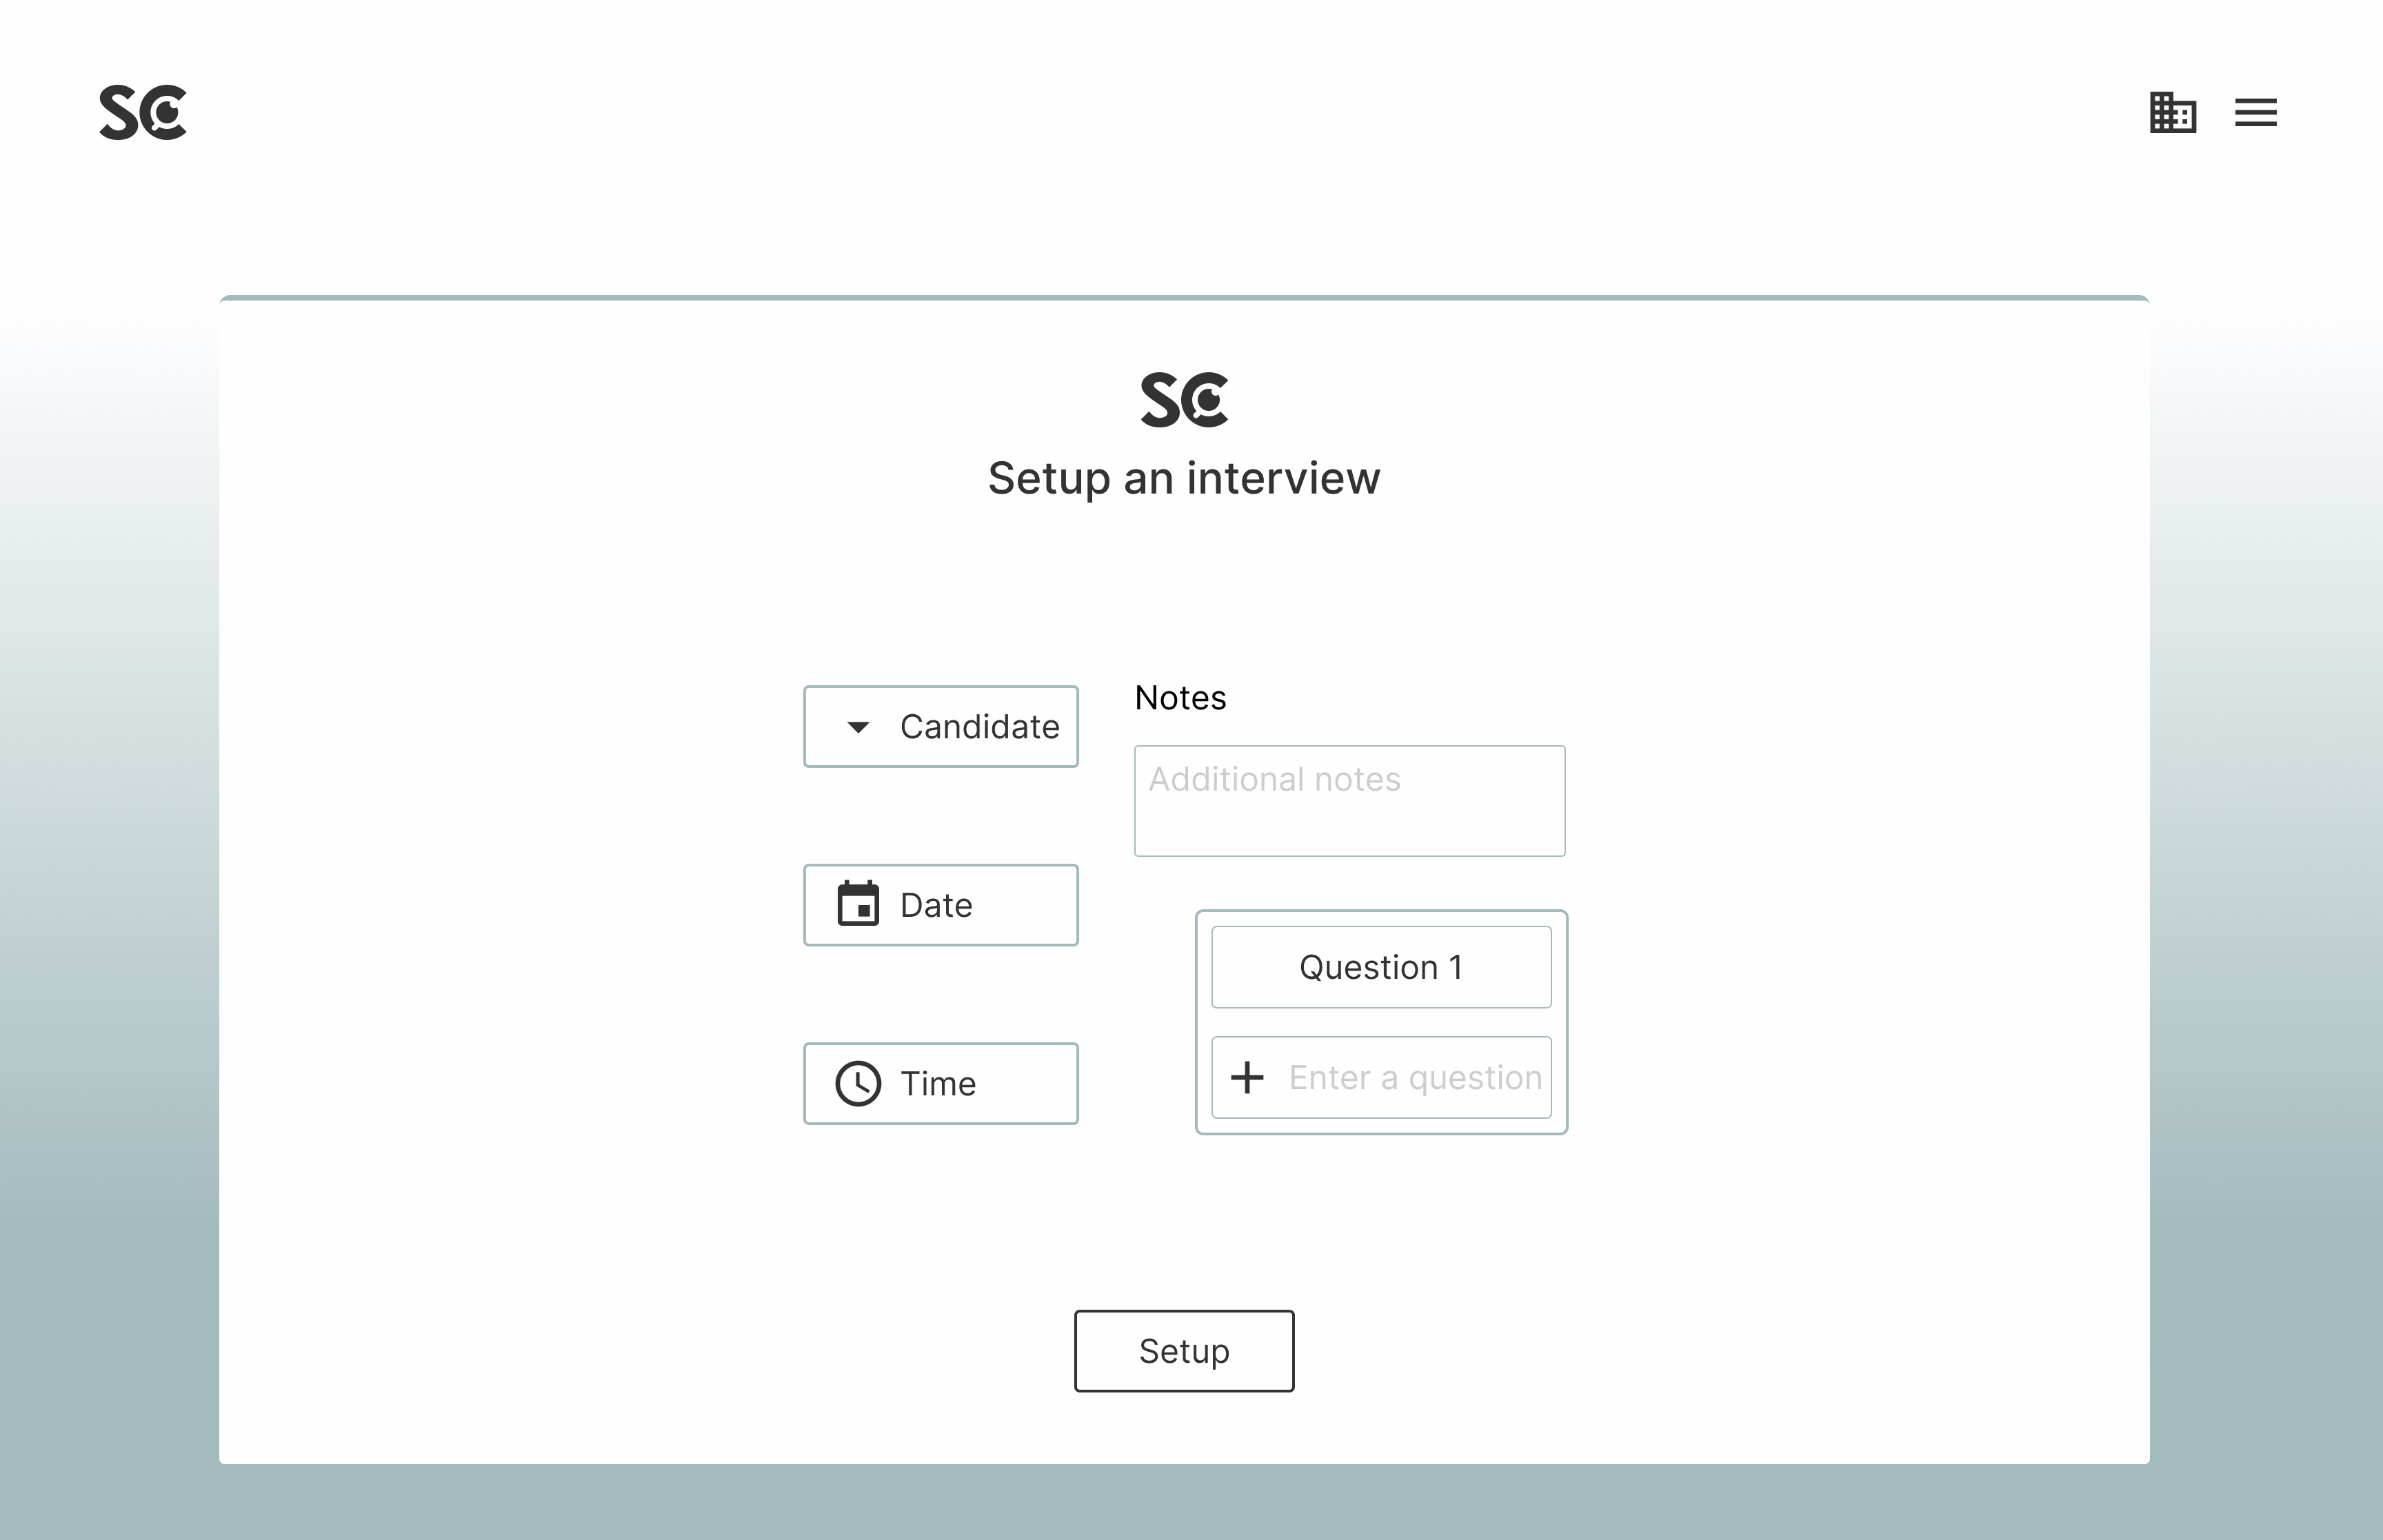
\includegraphics[width=0.8\textwidth]{Images/ui/Setup Interview}
%    \caption{Setup Interview}
%    \label{fig:setup}
%\end{figure}
%
%If we wanted to see all the planned interviews we would have a similar interface as the one for the student.
%In this case we have the classic list on the left with all the planned interviews, that can be filtered by date and via the searchbar.
%On the right side other than the interview information we can also see the candidate, with the possibility of clicking the Evaluate button, used to redirect to the Conduct Interview page, where we have additional tools that we can use to evaluate the student.
%\begin{figure}[H]
%    \centering
%    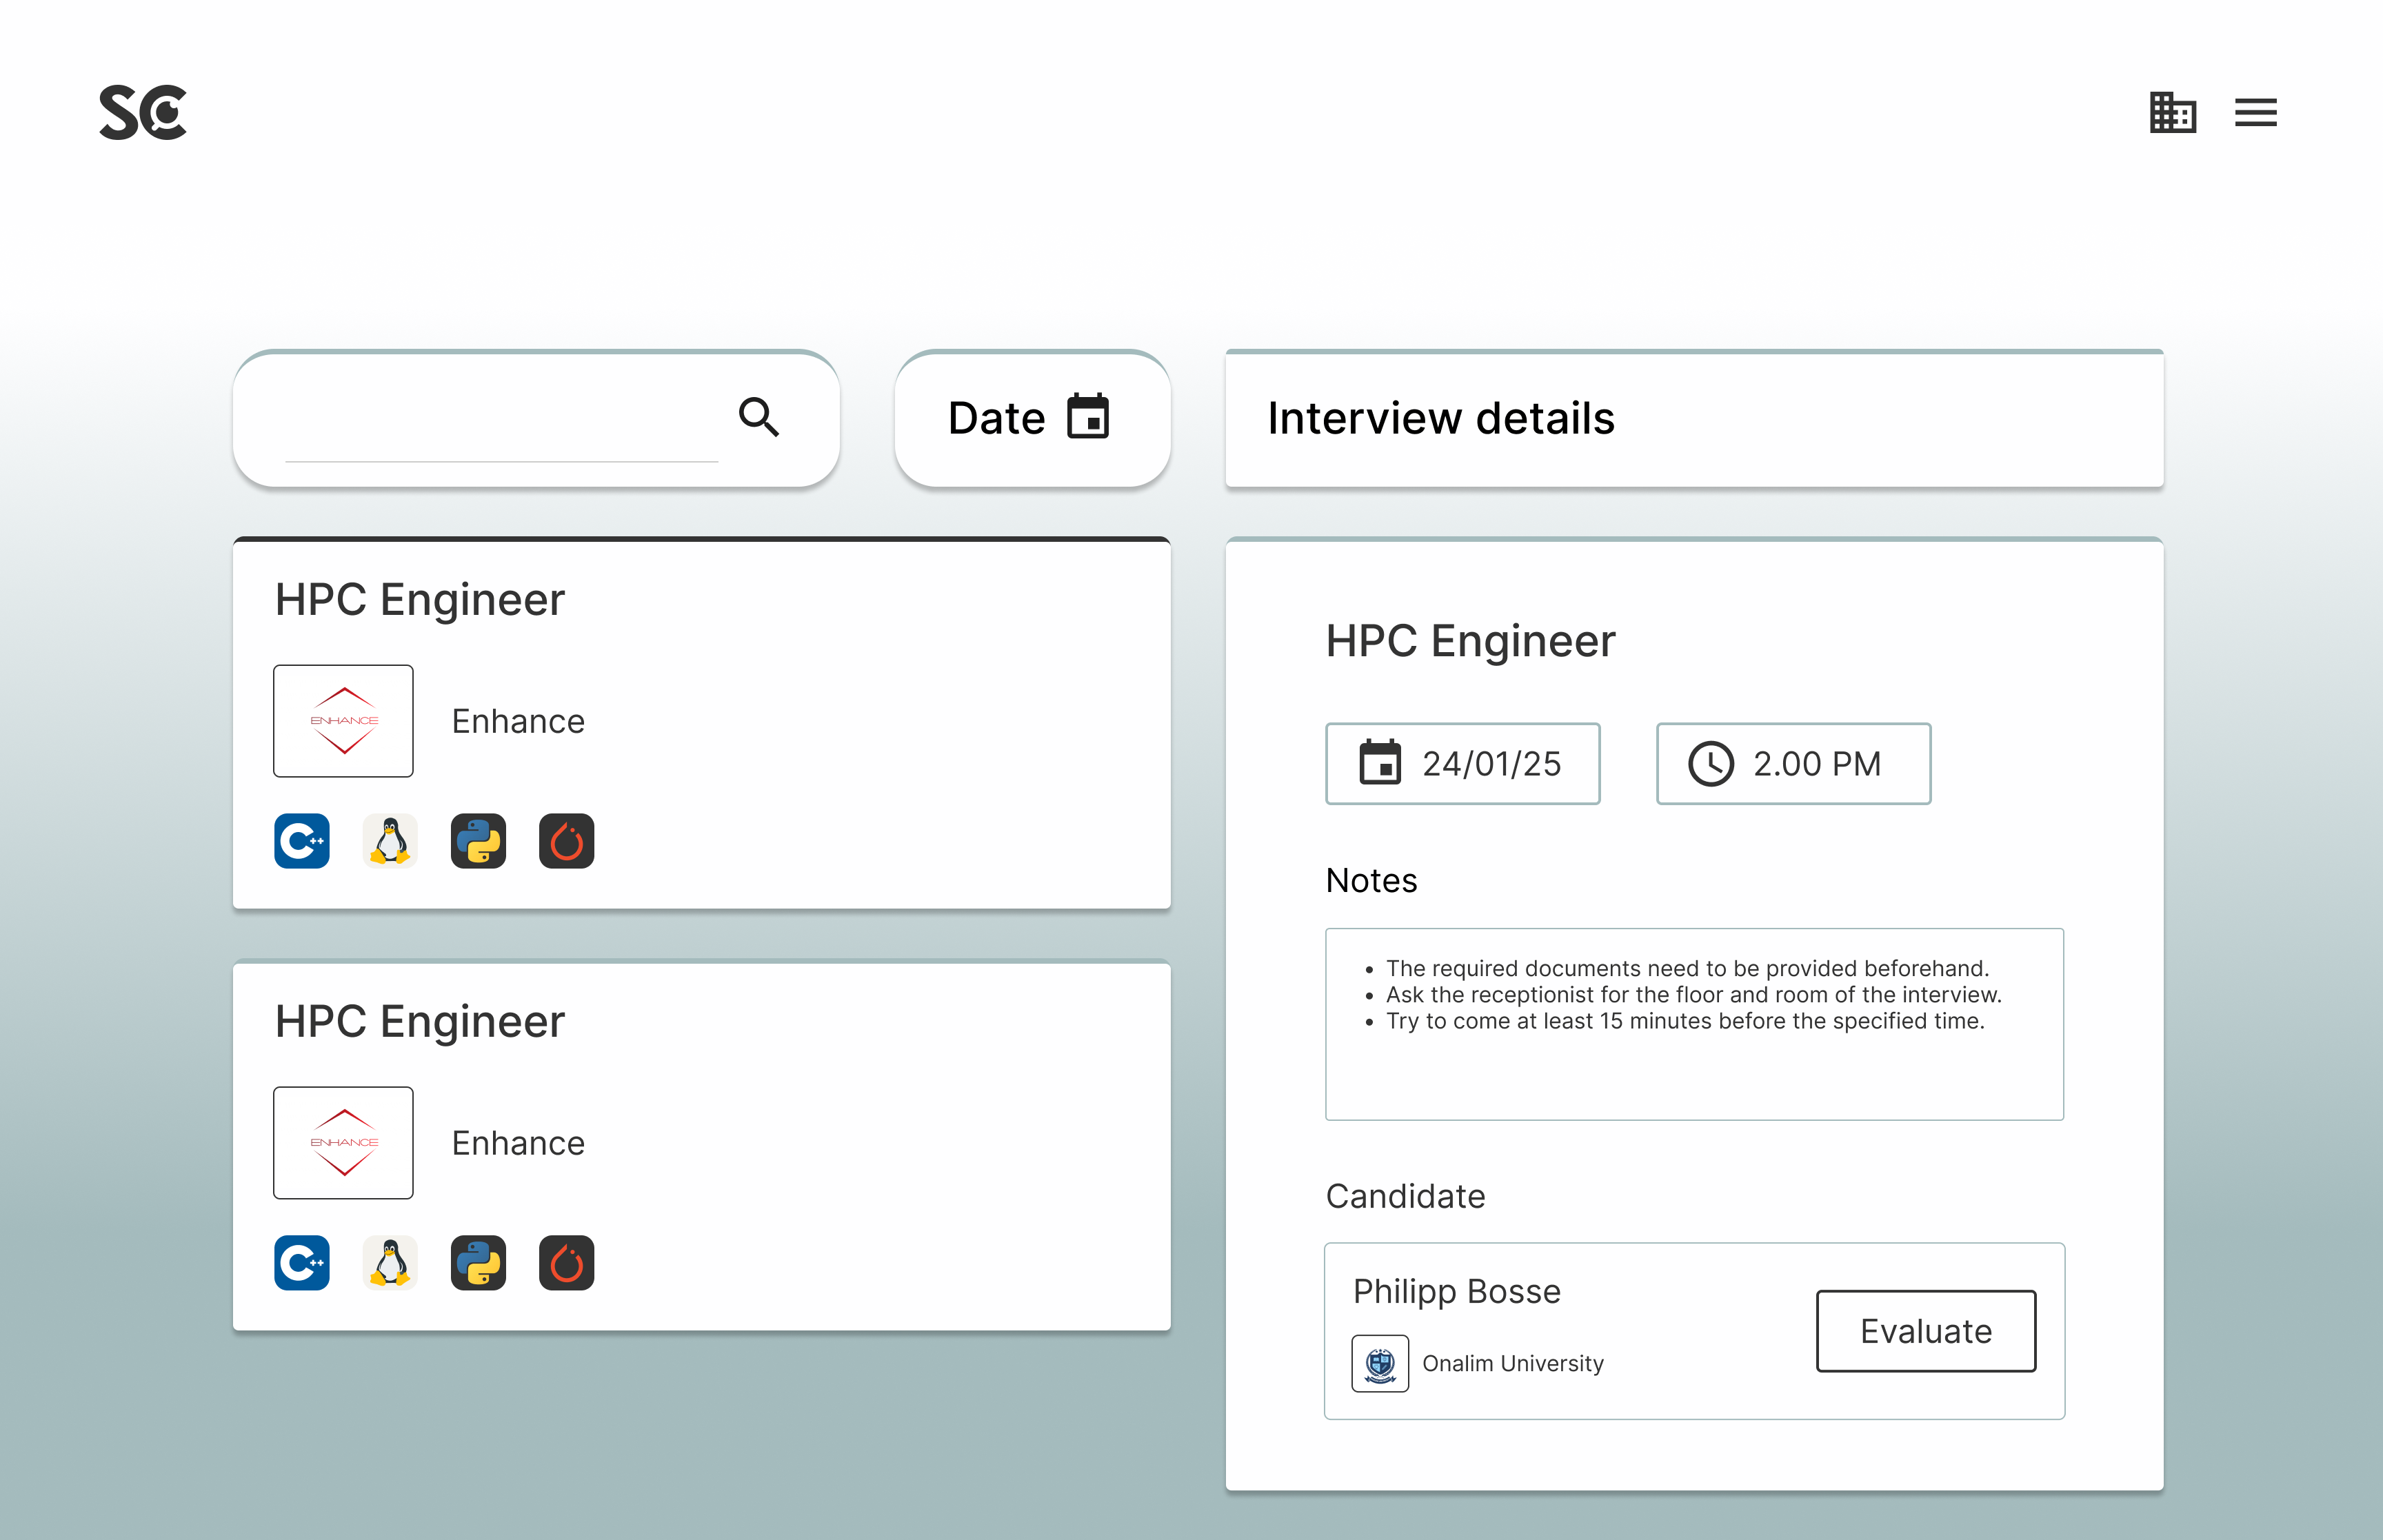
\includegraphics[width=0.8\textwidth]{Images/ui/View Planned interviews Company}
%    \caption{View Planned Interviews}
%    \label{fig:plannedIntCompany}
%\end{figure}
%
%If we actually use the Evaluate button we would be shown the following interface.
%On the left we have the candidate with some basic information, underneath we can assign scores ranging from 1 to 10 to the candidate in three different categories.
%On the right we can write some additional notes regarding the interview evaluation.
%To finish the evaluation process simply click on the Confirm button.
%\begin{figure}[H]
%    \centering
%    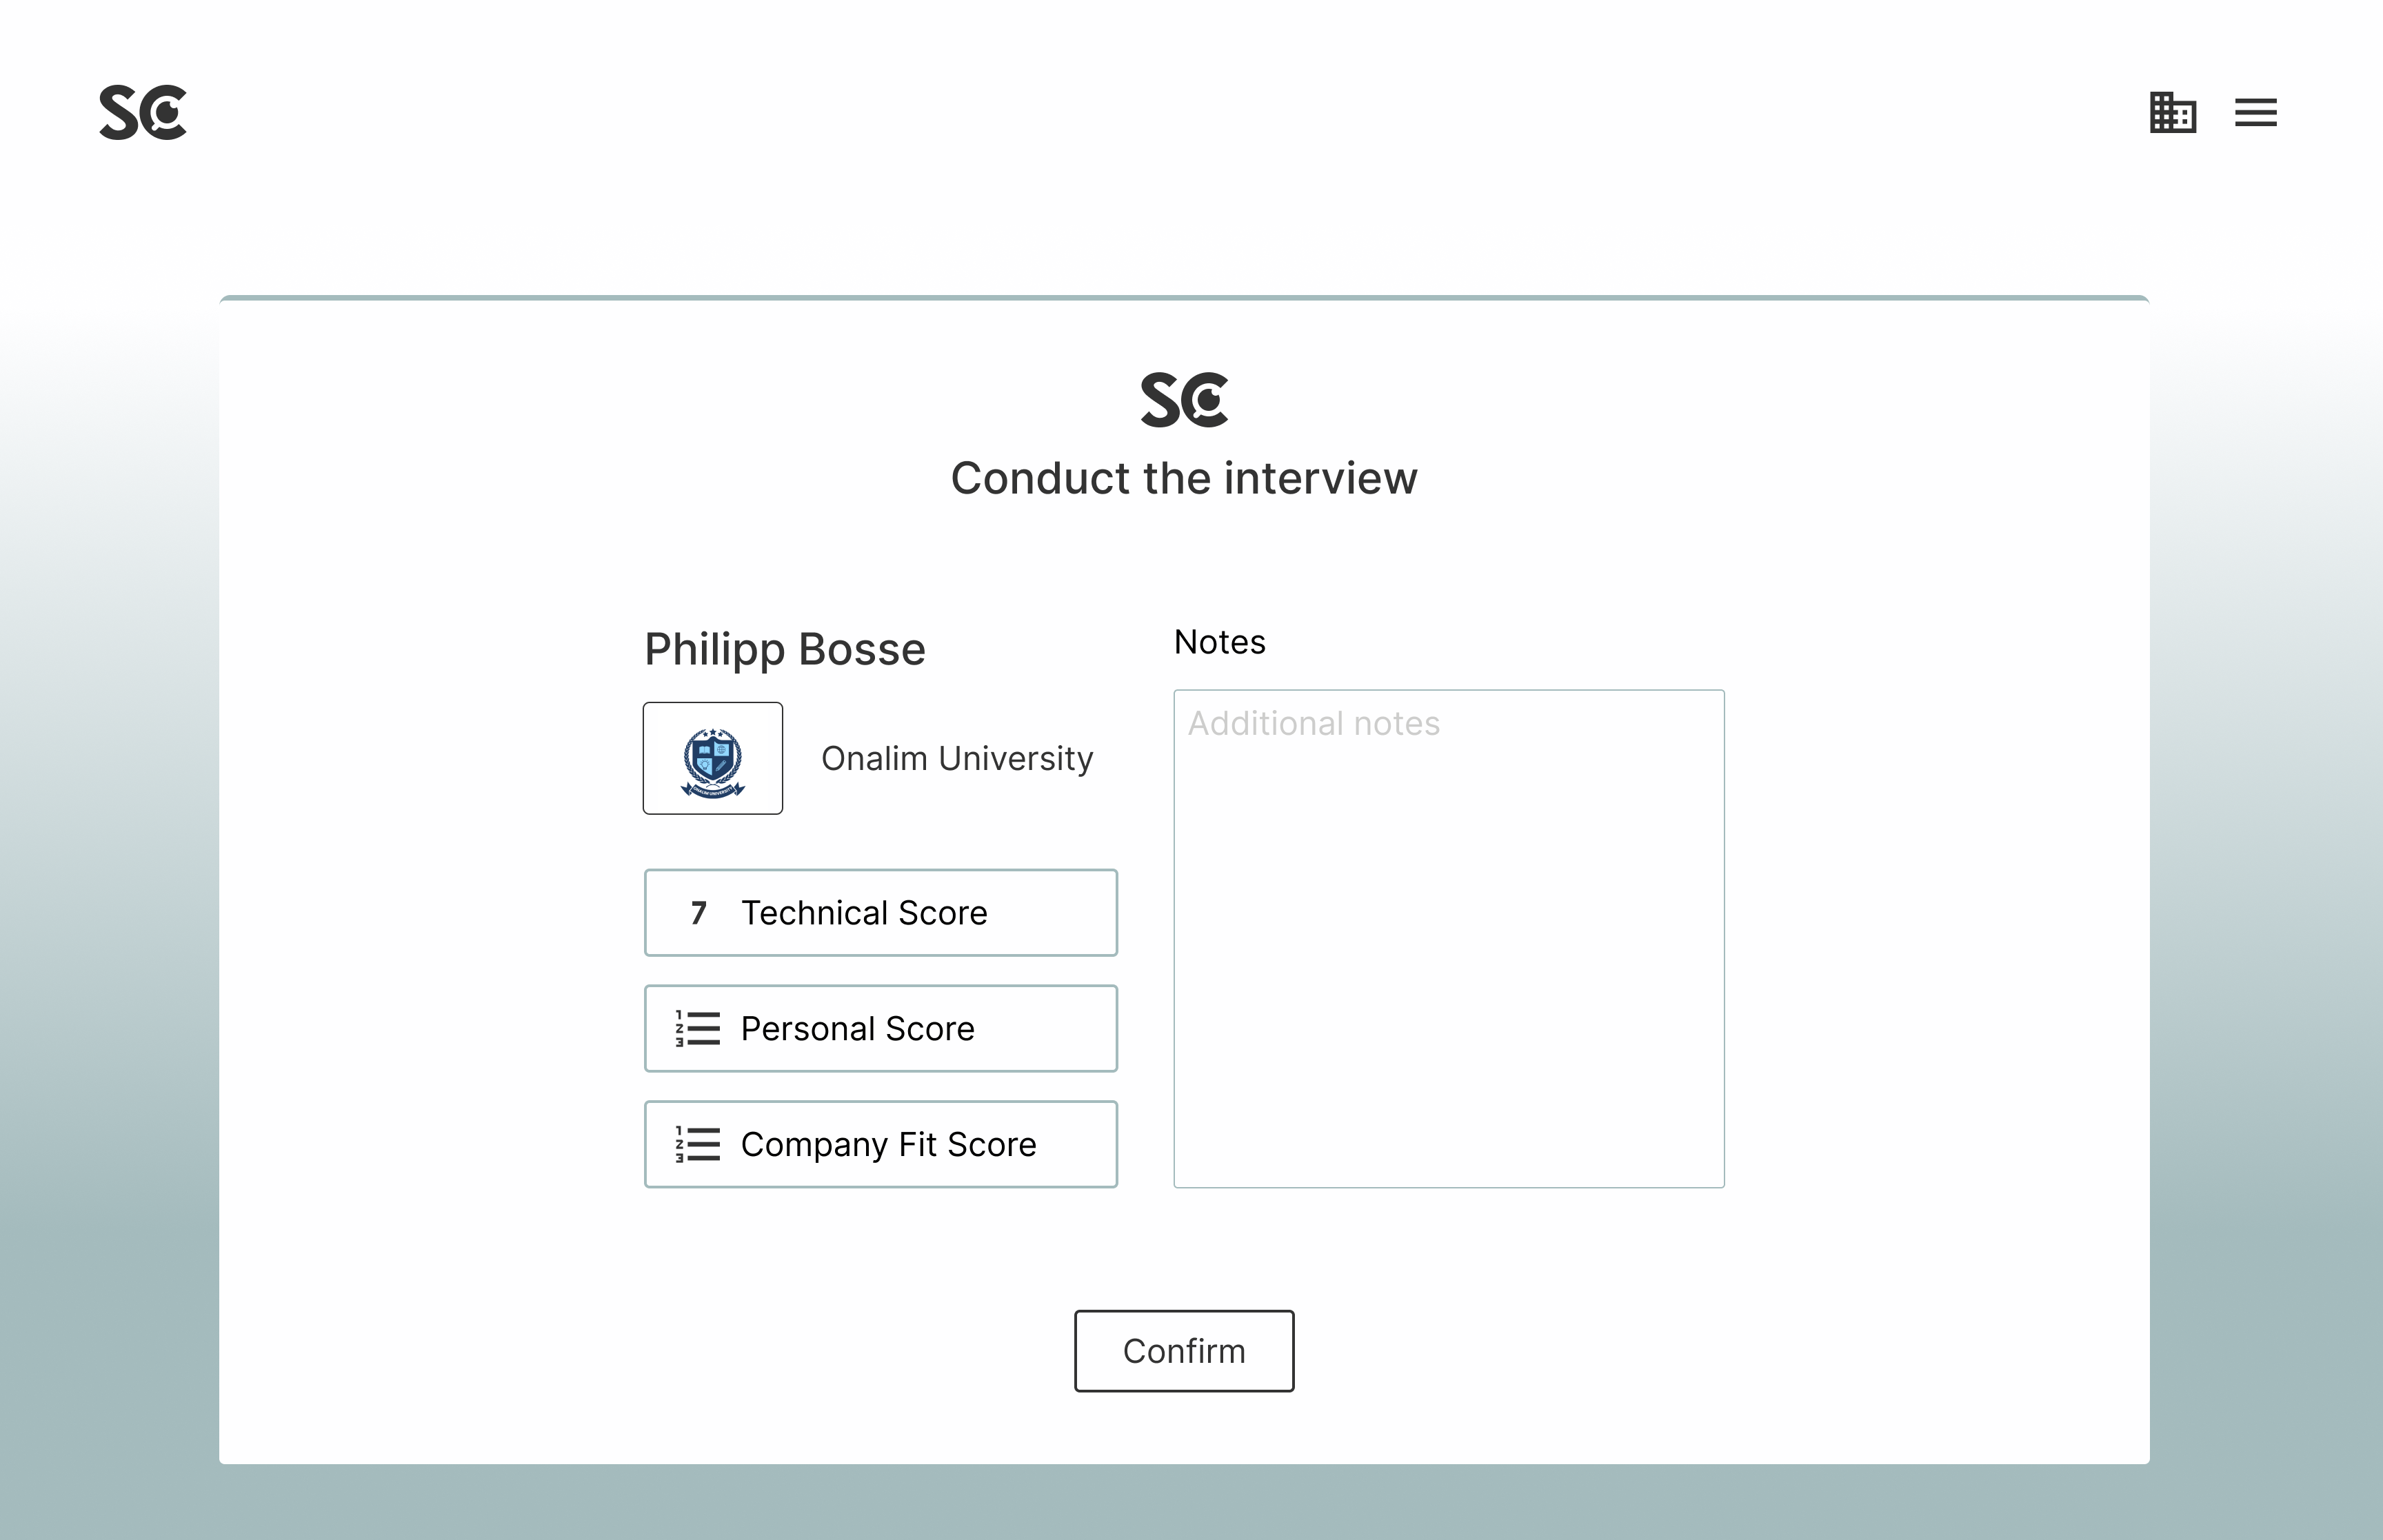
\includegraphics[width=0.8\textwidth]{Images/ui/Conduct Interview}
%    \caption{Conduct Interview}
%    \label{fig:conduct}
%\end{figure}
%
%Once we finished evaluating all the candidates for a position, we can navigate to the View Published Internship page, where by selecting the appropriate internship we can click on the Finalize button.
%This initiates the finalize selection process of the candidates.
%In this interface we can see all the evaluated candidates on the left, sorted by evaluation score.
%If we select one of the students we can see on the right hand side the answers to all the questions posed in the structured questioner, as well as a button that we can use to select the candidate as the chosen one.
%\begin{figure}[H]
%    \centering
%    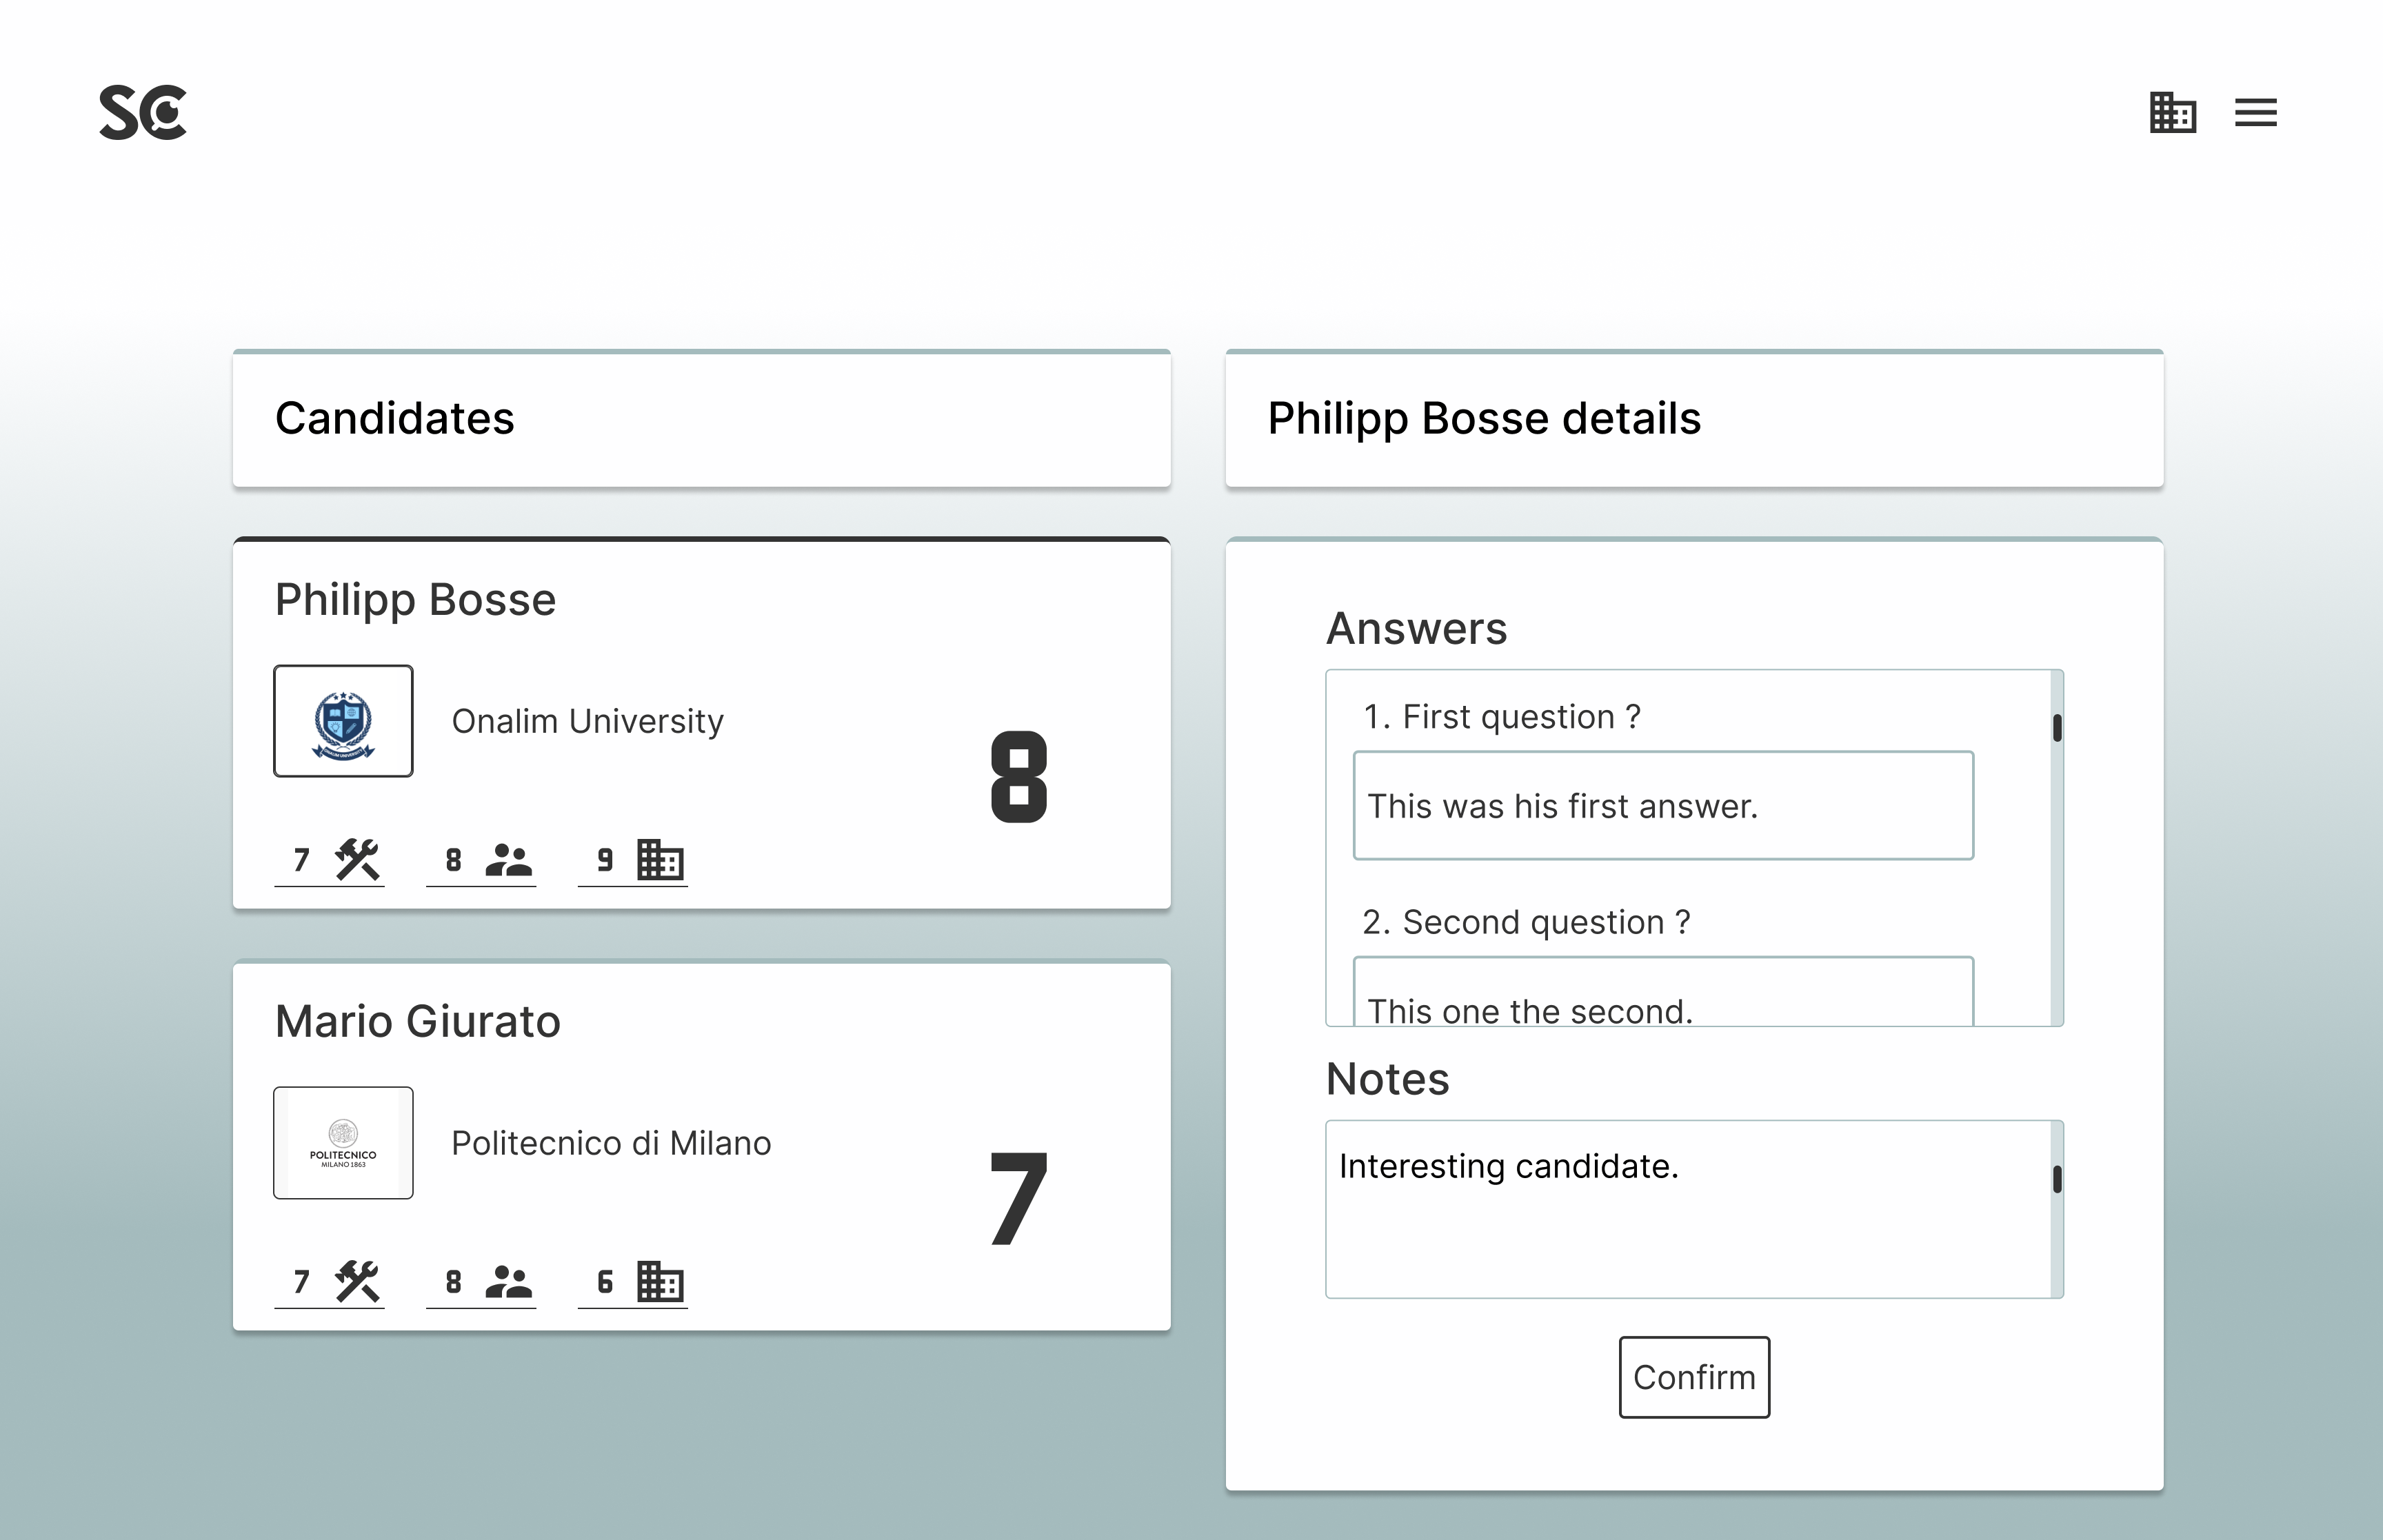
\includegraphics[width=0.8\textwidth]{Images/ui/Finalize Selection}
%    \caption{Finalize Selection}
%    \label{fig:finalize}
%\end{figure}
%
%To access all the previous interfaces we opted for a side menu, as we did with the Student interface, that can be accessed through the hamburger icon in the top right corner of the interface.
%Once the menu is opened, we can simply click on the desired functionality.
%\begin{figure}[H]
%    \centering
%    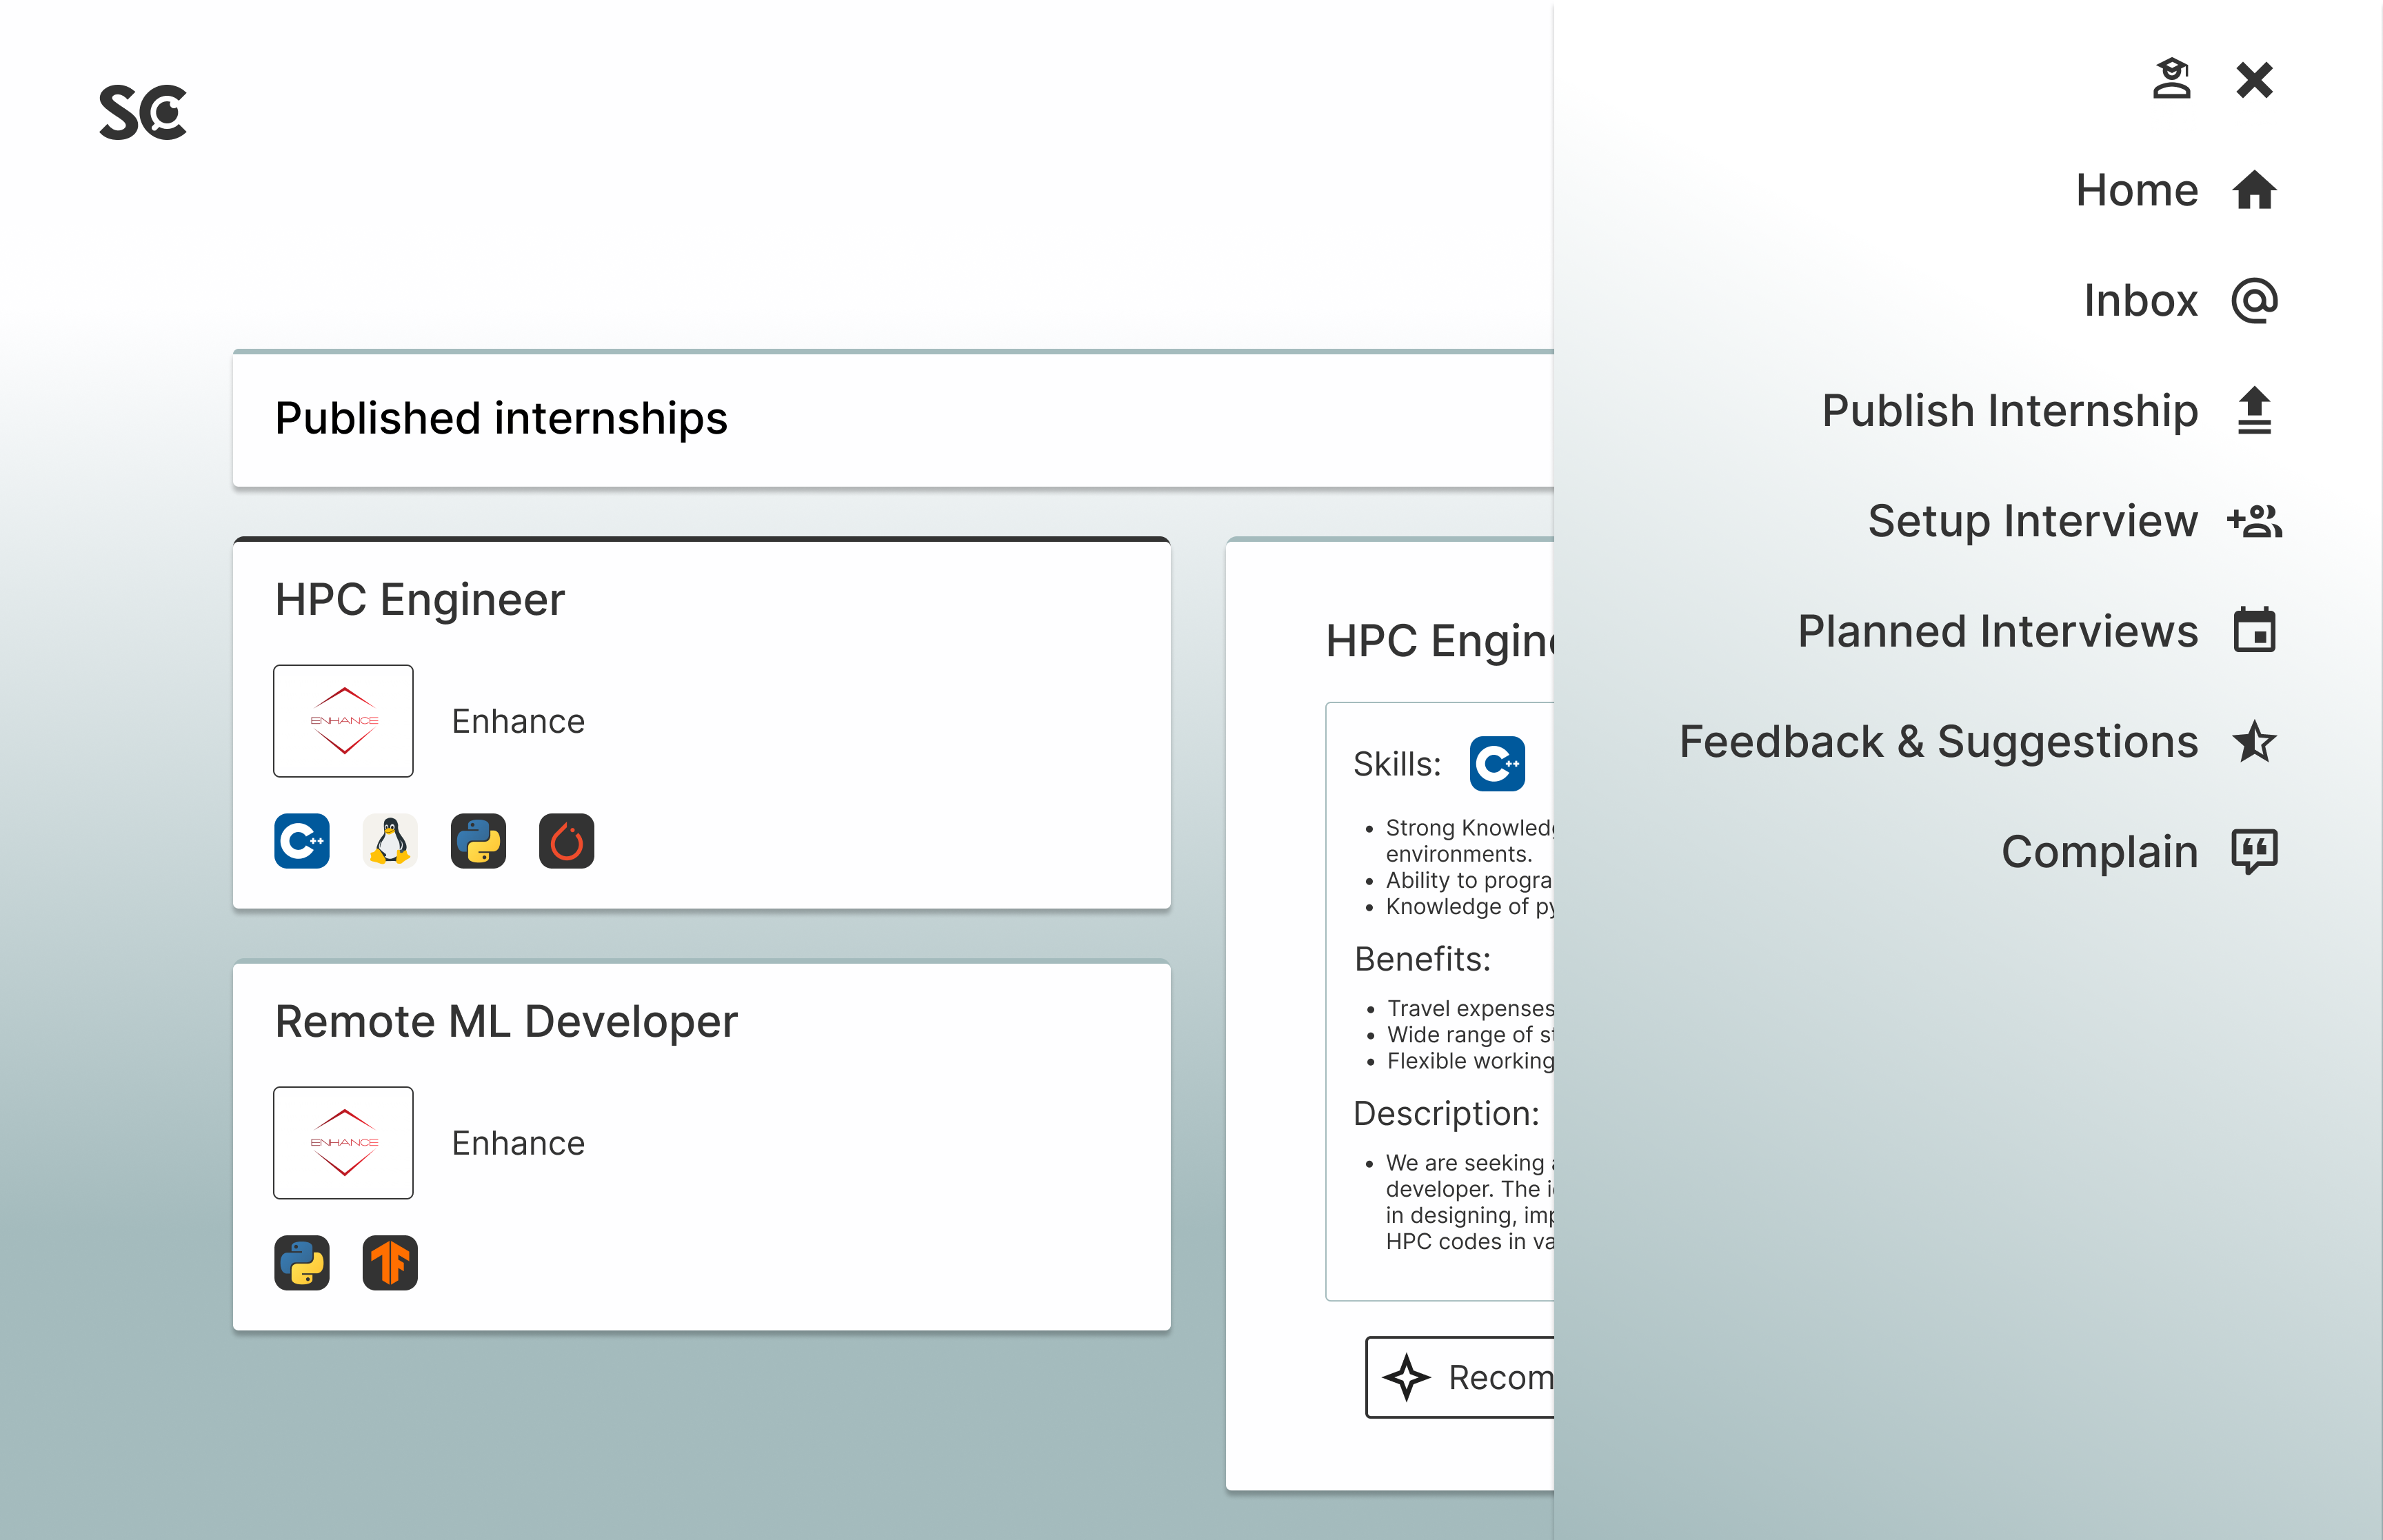
\includegraphics[width=0.8\textwidth]{Images/ui/Sidebar Company}
%    \caption{Company Menu}
%    \label{fig:companyMenu}
%\end{figure}
%
%
%\section{Shared Interfaces}\label{sec:shared-interfaces}
%In this section is provided the description of the shared functionalities of Students and Companies.
%
%The first one is the Complain page, where users can express all the problems and concerns regarding an internship.
%The flow is:
%\begin{itemize}
%    \item Pick the internship via the dropdown menu at the top
%    \item Complete the message
%    \item Click on the publish button
%\end{itemize}
%\begin{figure}[H]
%    \centering
%    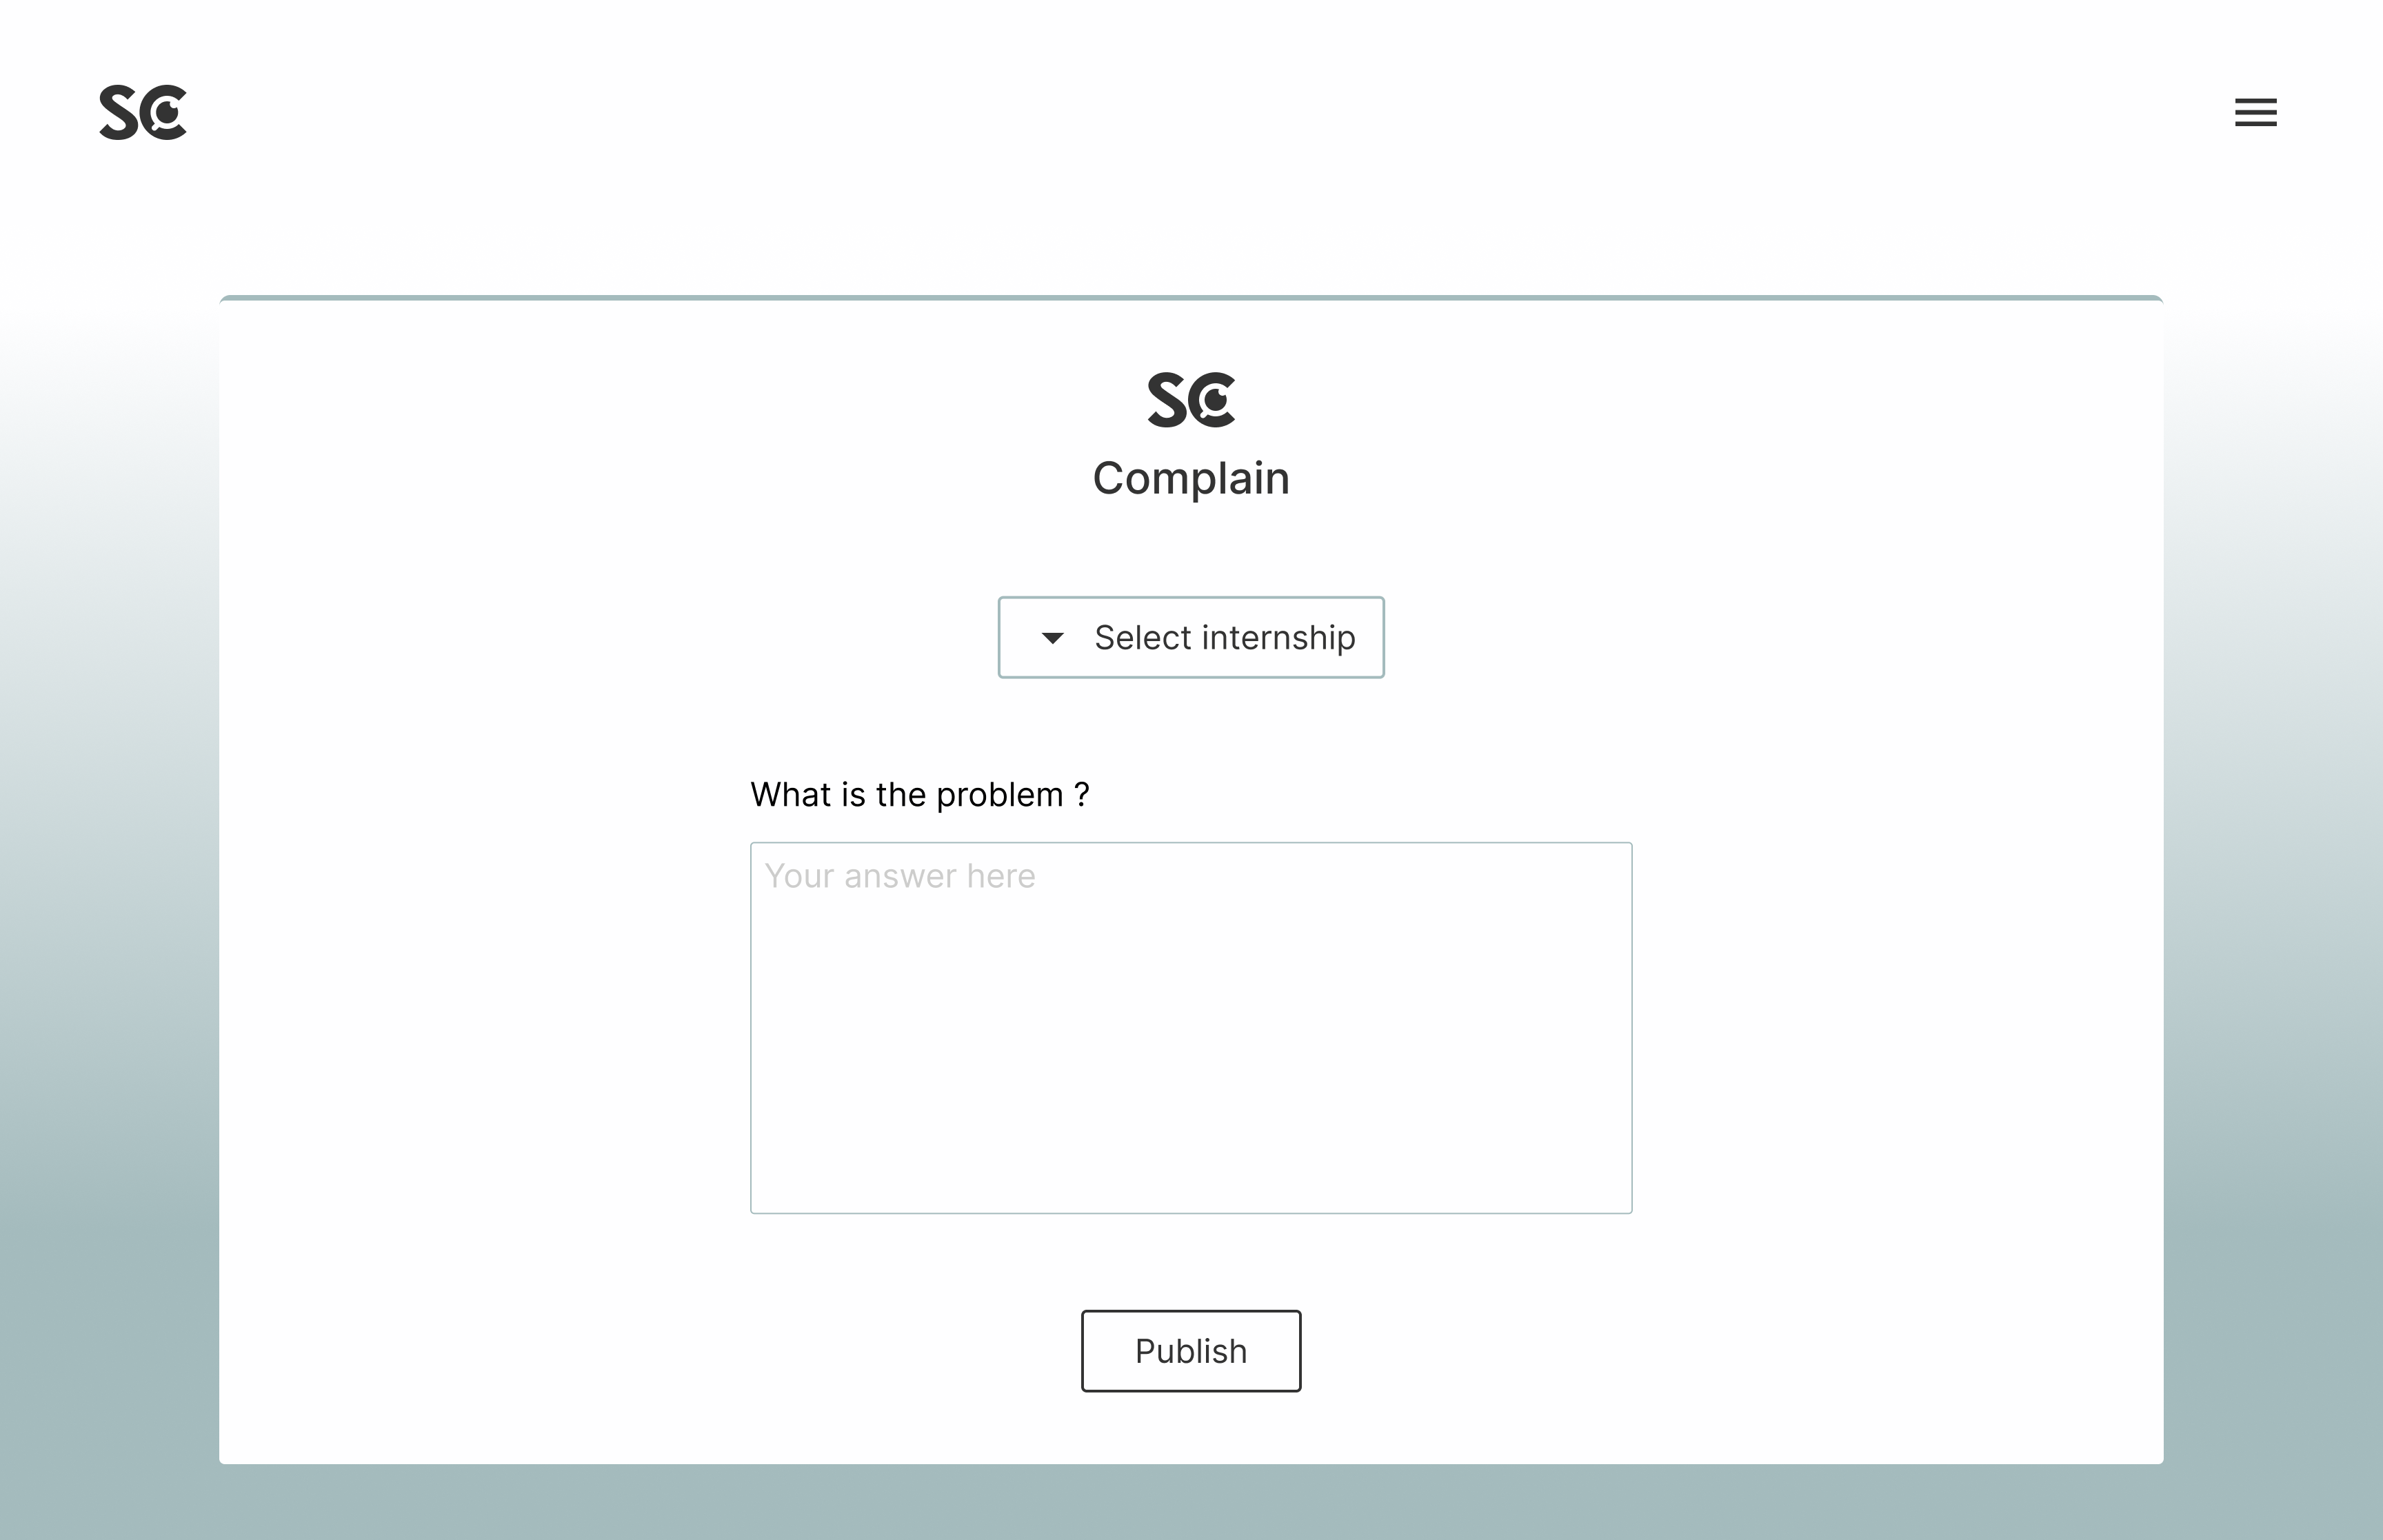
\includegraphics[width=0.8\textwidth]{Images/ui/Complain}
%    \caption{Complain}
%    \label{fig:complain}
%\end{figure}
%
%The second interface is the Feedback and Suggestions page, where the System collects information form Students and Companies to feed the Analysis Tool.
%The required actions are to respond to the question and give a rating out of 5 stars.
%\begin{figure}[H]
%    \centering
%    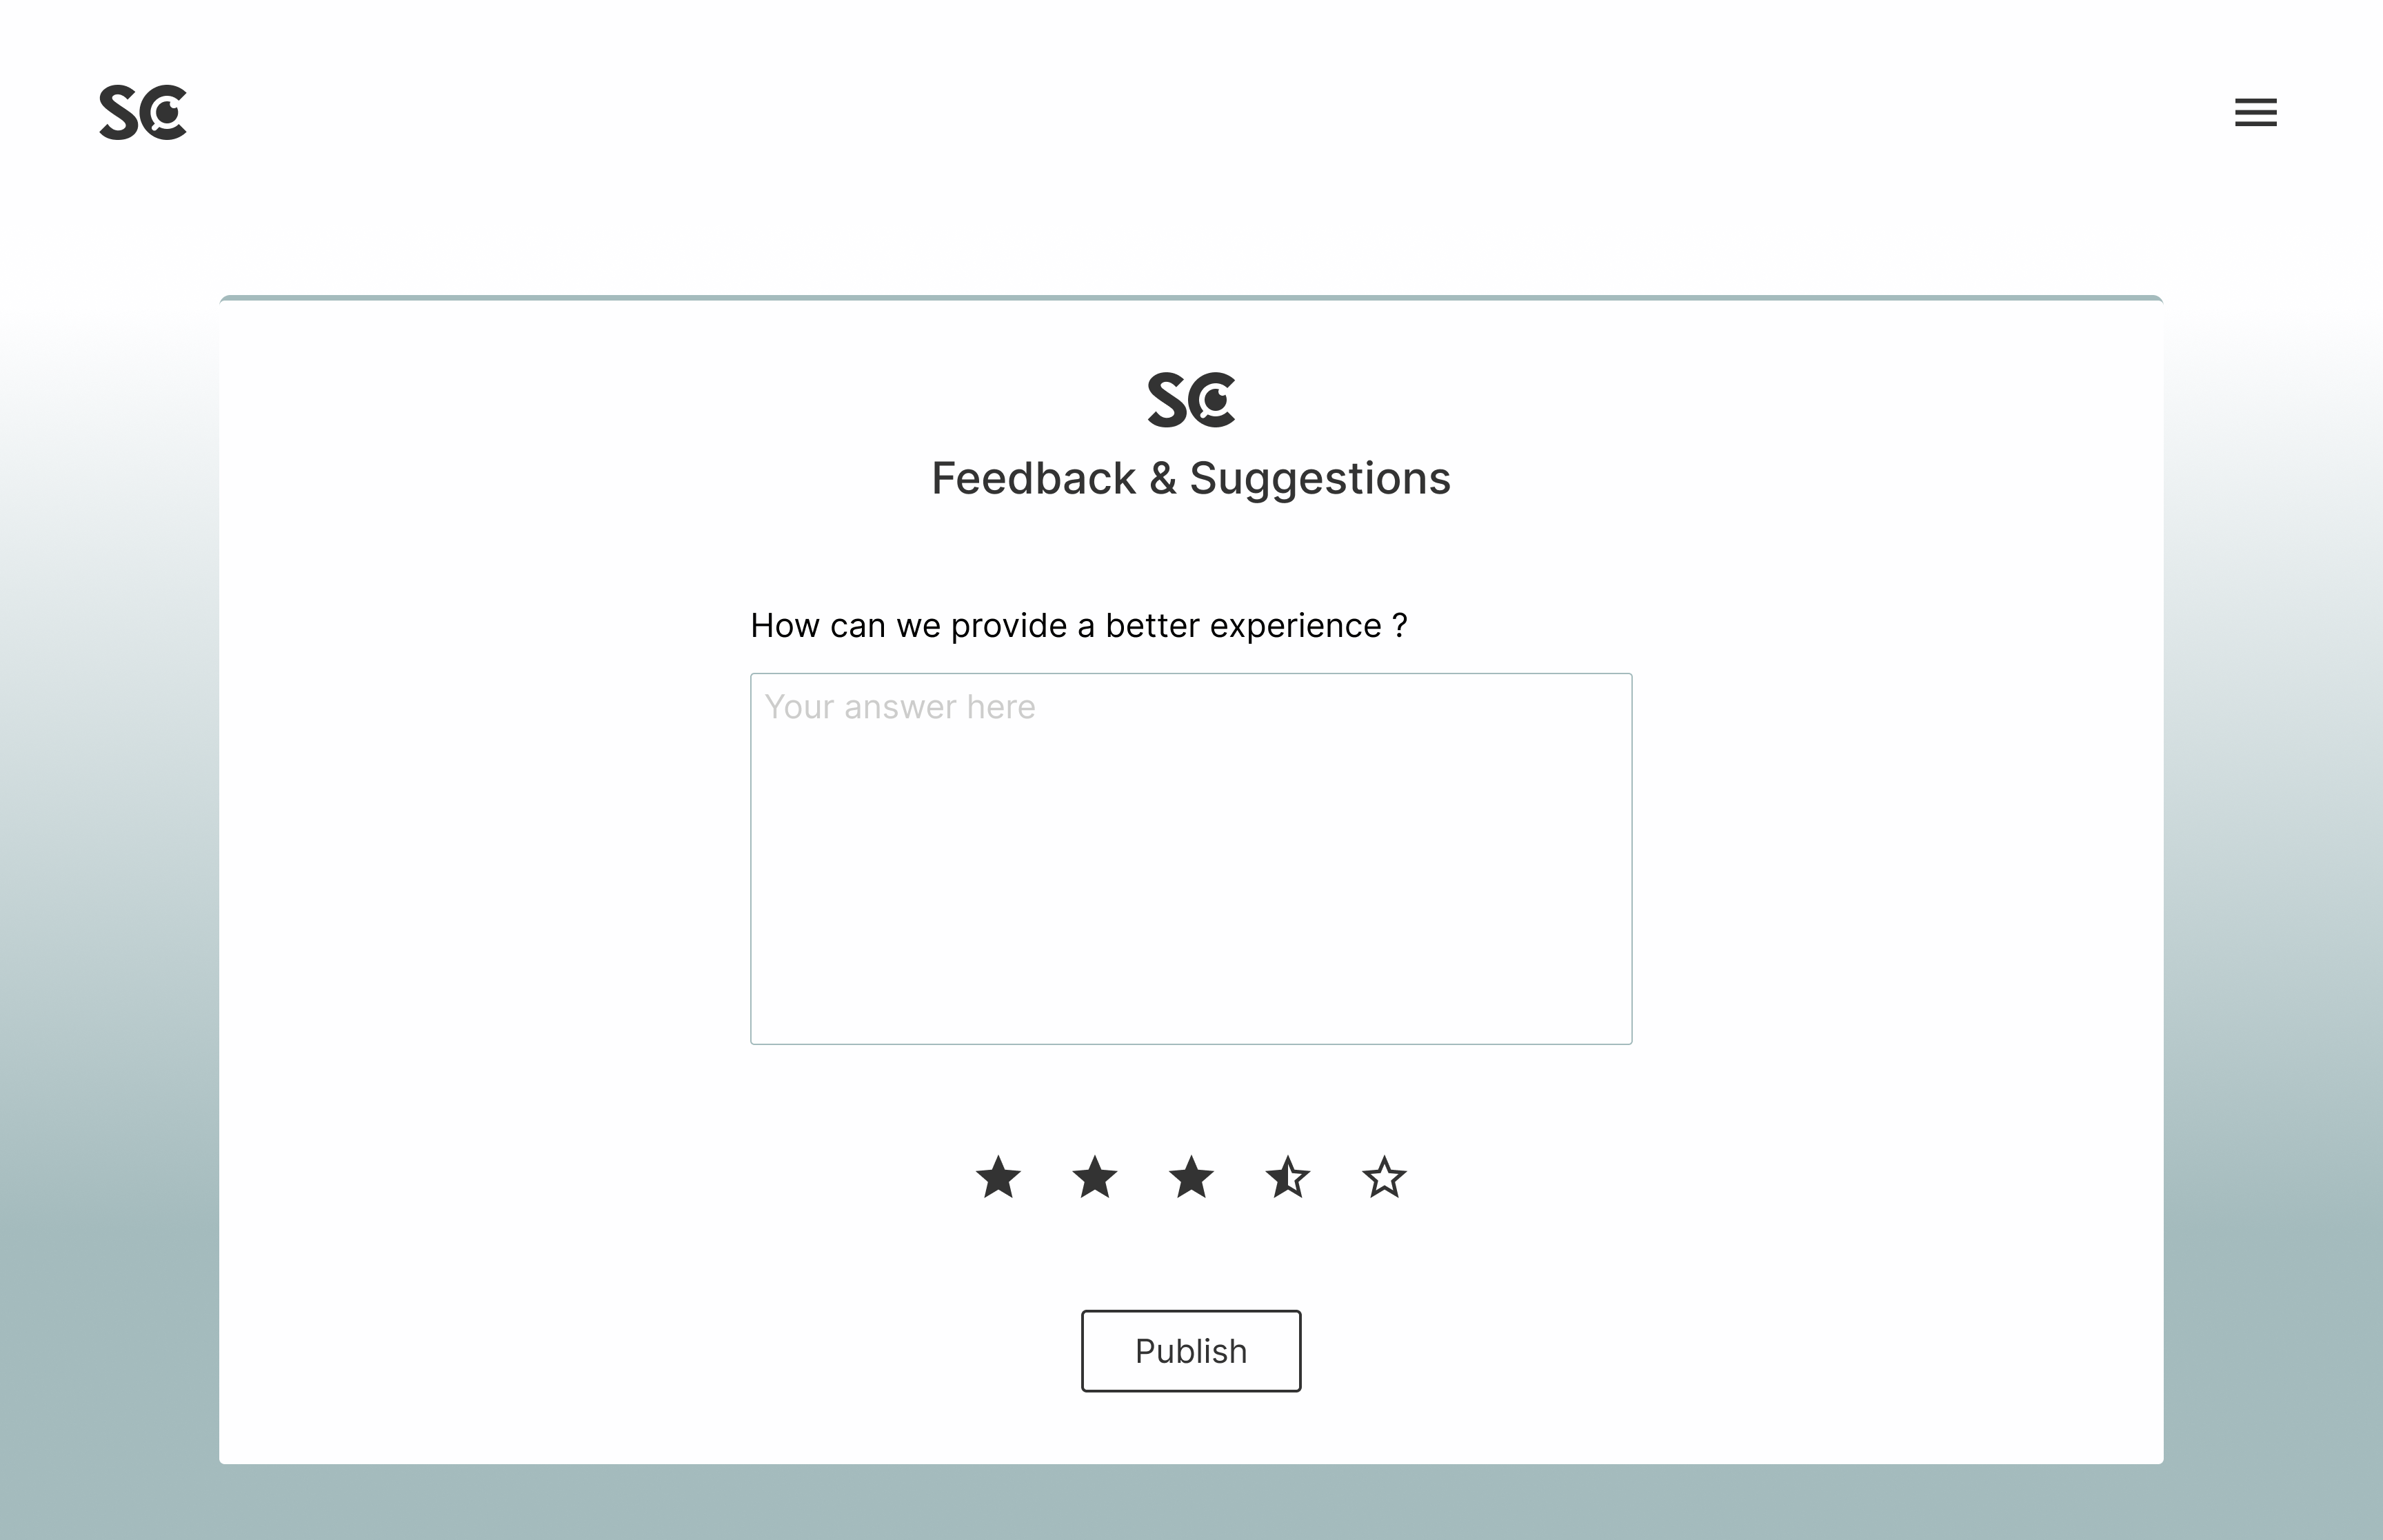
\includegraphics[width=0.8\textwidth]{Images/ui/Feedback & Suggestions}
%    \caption{Feedback and Suggestions}
%    \label{fig:feedback}
%\end{figure}
%
%\section{University Interface}\label{sec:university-interface}
%The main role of universities is to oversee the internships, this can be done via the Handle Complaints page.
%Here we can select on the left side the internship for which we want to see the complaints.
%On the right we can see the Company and Student names, as well as all the relevant complaints for that internship.
%A complaint has the sender, a body  and a message box where the University can provide a response.
%\begin{figure}[H]
%    \centering
%    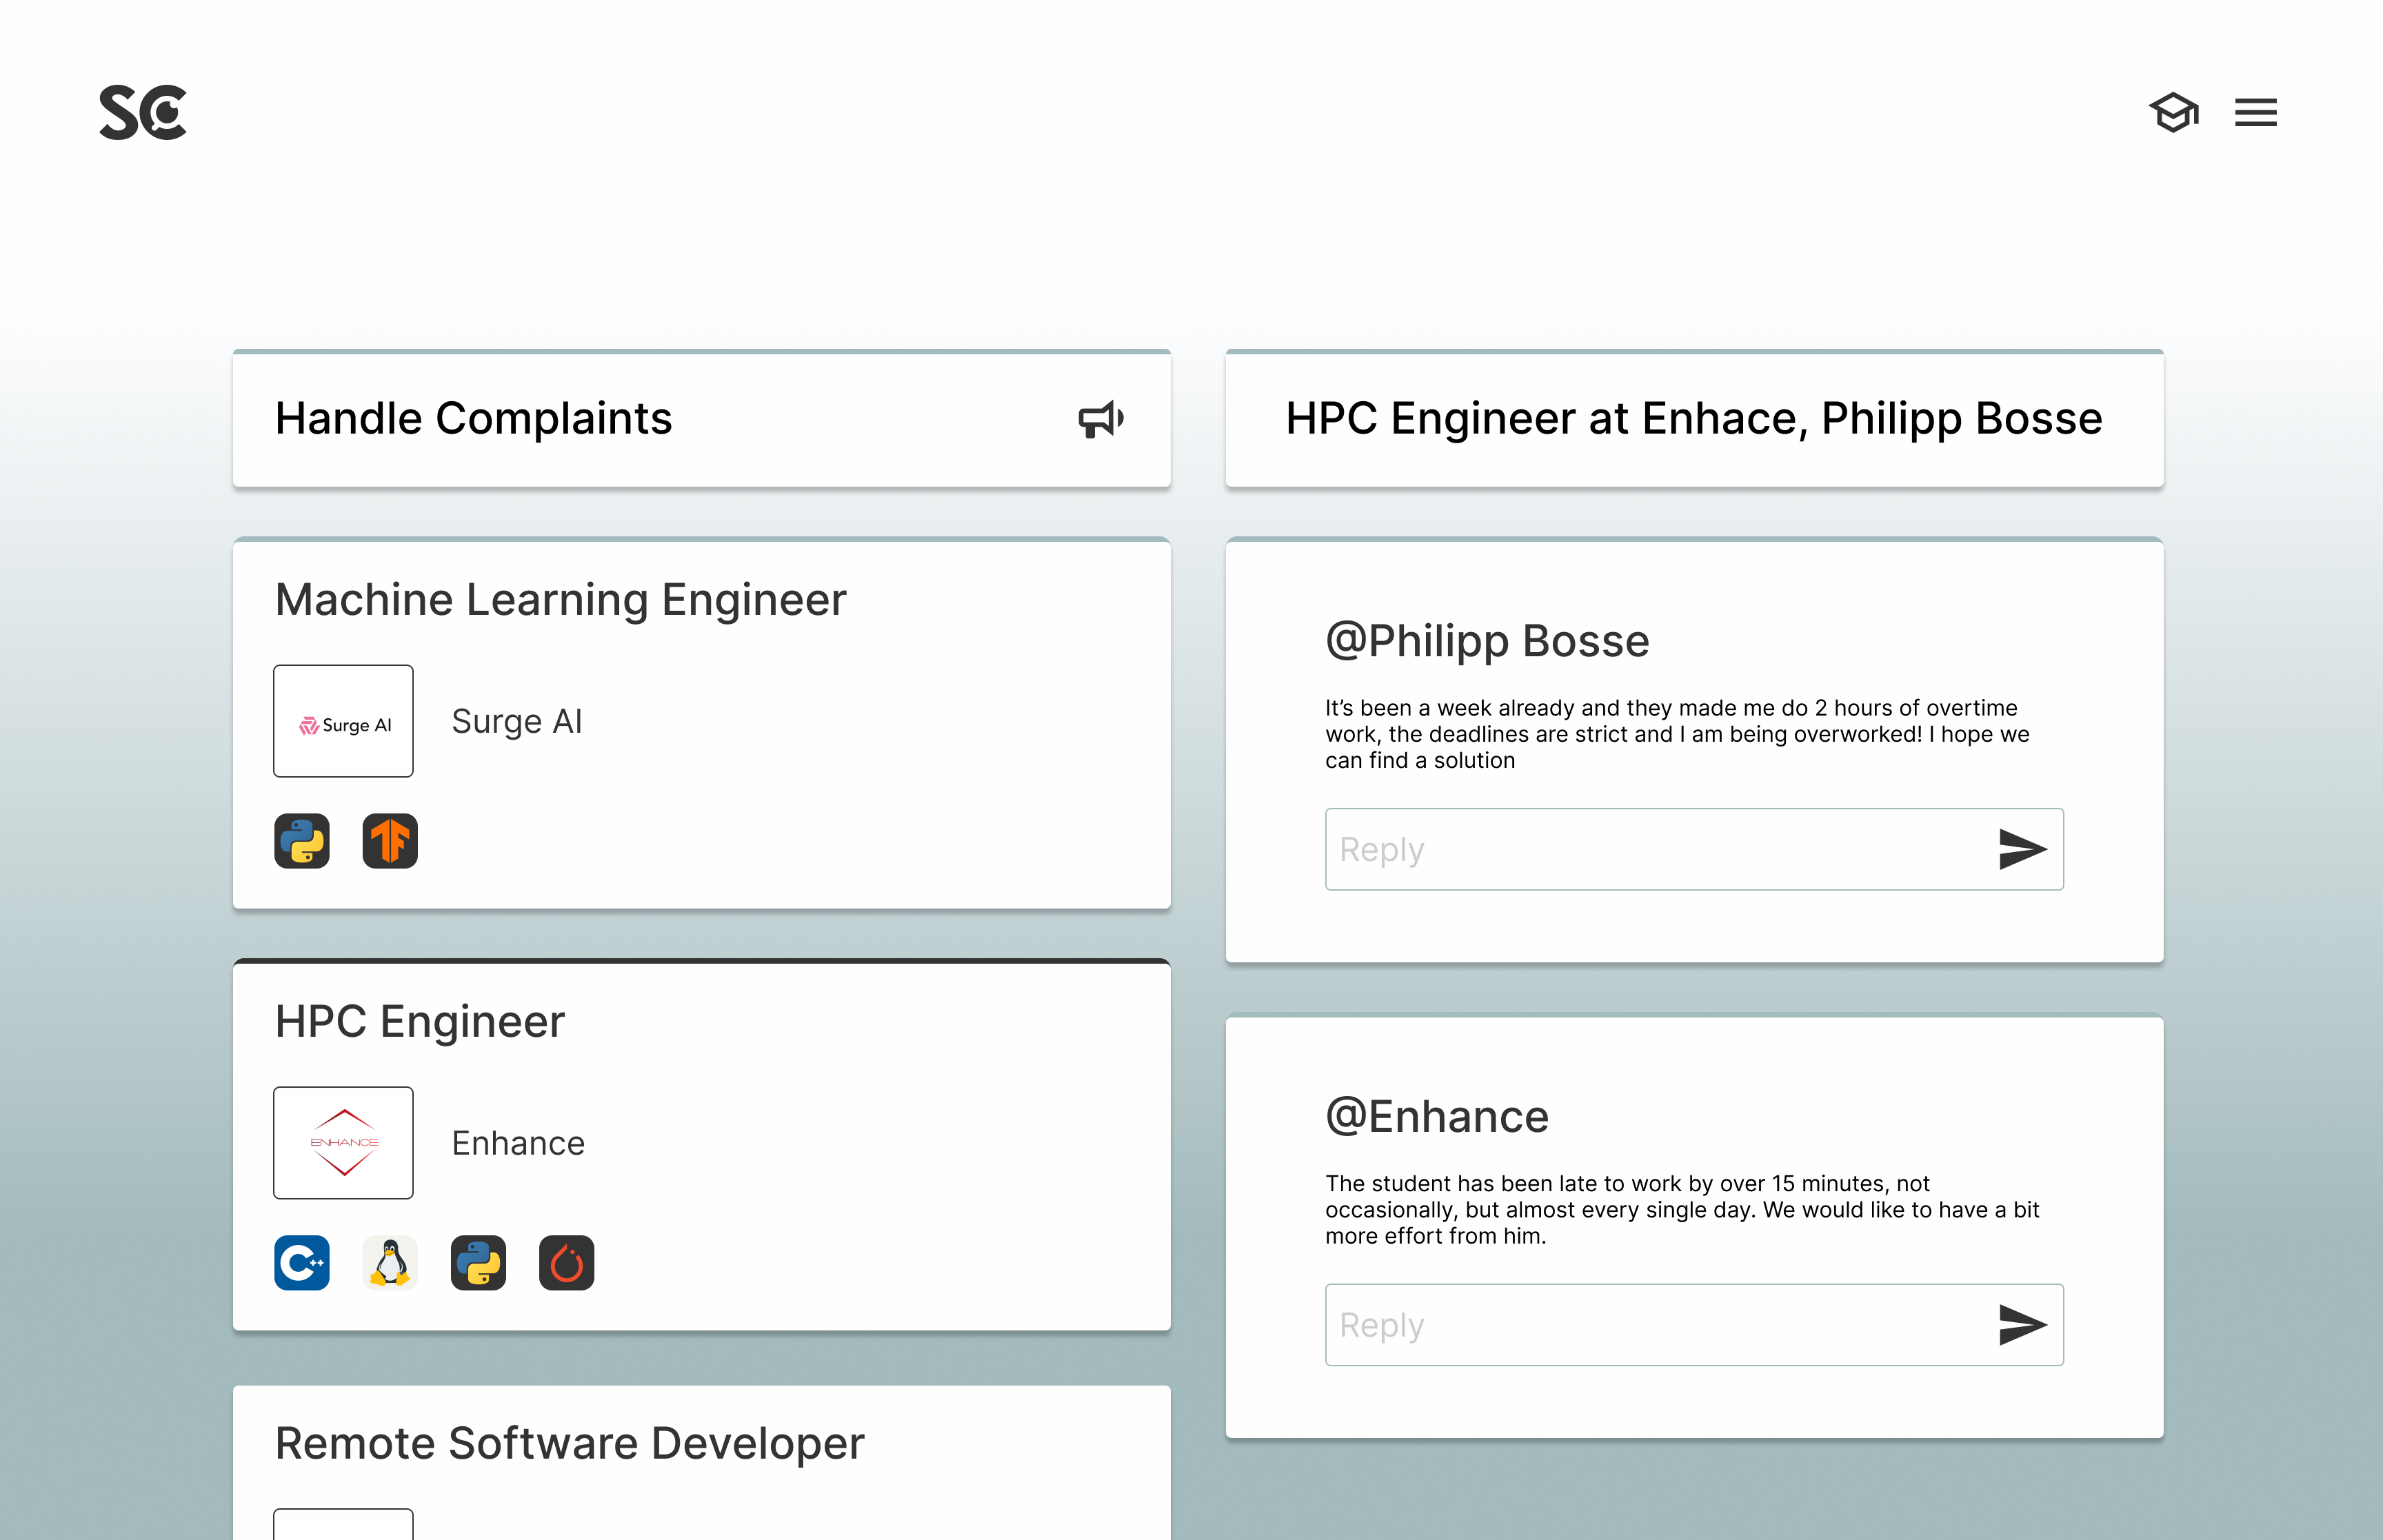
\includegraphics[width=0.8\textwidth]{Images/ui/View Complaints}
%    \caption{Handle Complaints}
%    \label{fig:handleComplaints}
%\end{figure}
%
%The University has also the authority to terminate an internship, and to do so it can navigate to the Terminate Internships page.
%Here the interface is similar to the previous one, but with the difference that once an internship is selected we can provide a reason of termination and click on the button to terminate the internship.
%\begin{figure}[H]
%    \centering
%    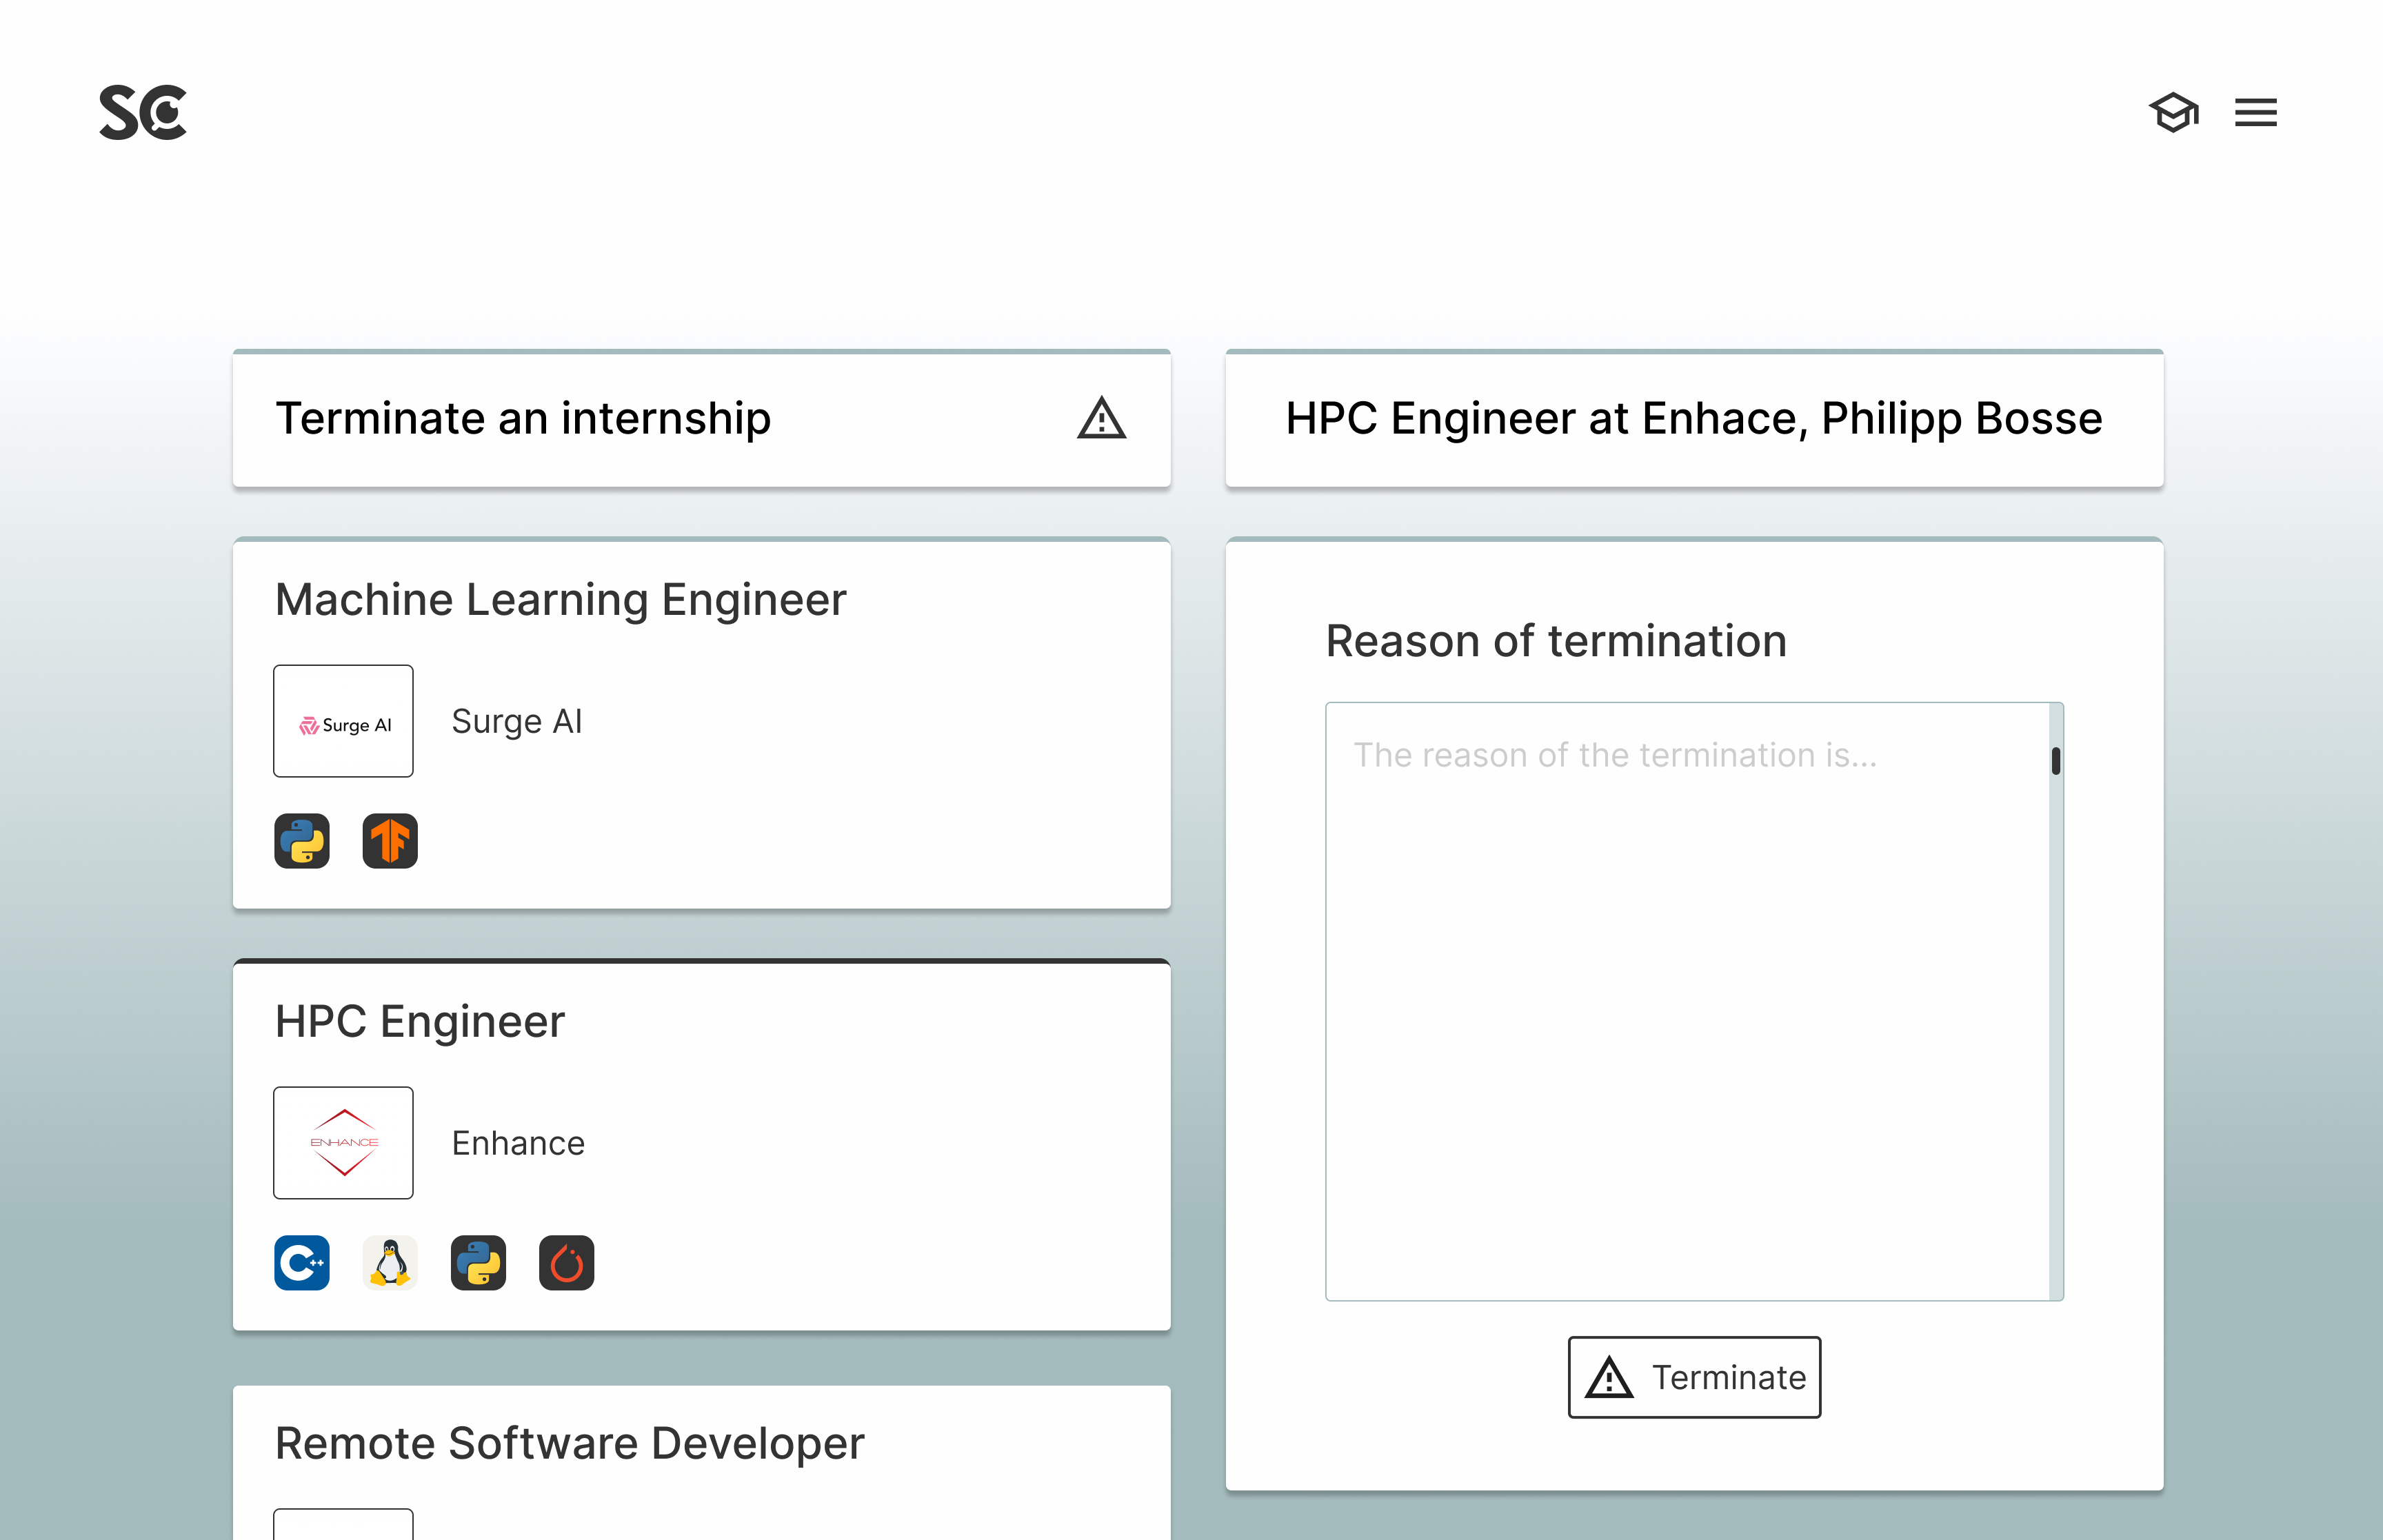
\includegraphics[width=0.8\textwidth]{Images/ui/Terminate Internship}
%    \caption{Terminate Internship}
%    \label{fig:terminate}
%\end{figure}
%
%To access both this functionalities we designed a side menu as we did for Companies and Students.
%\begin{figure}[H]
%    \centering
%    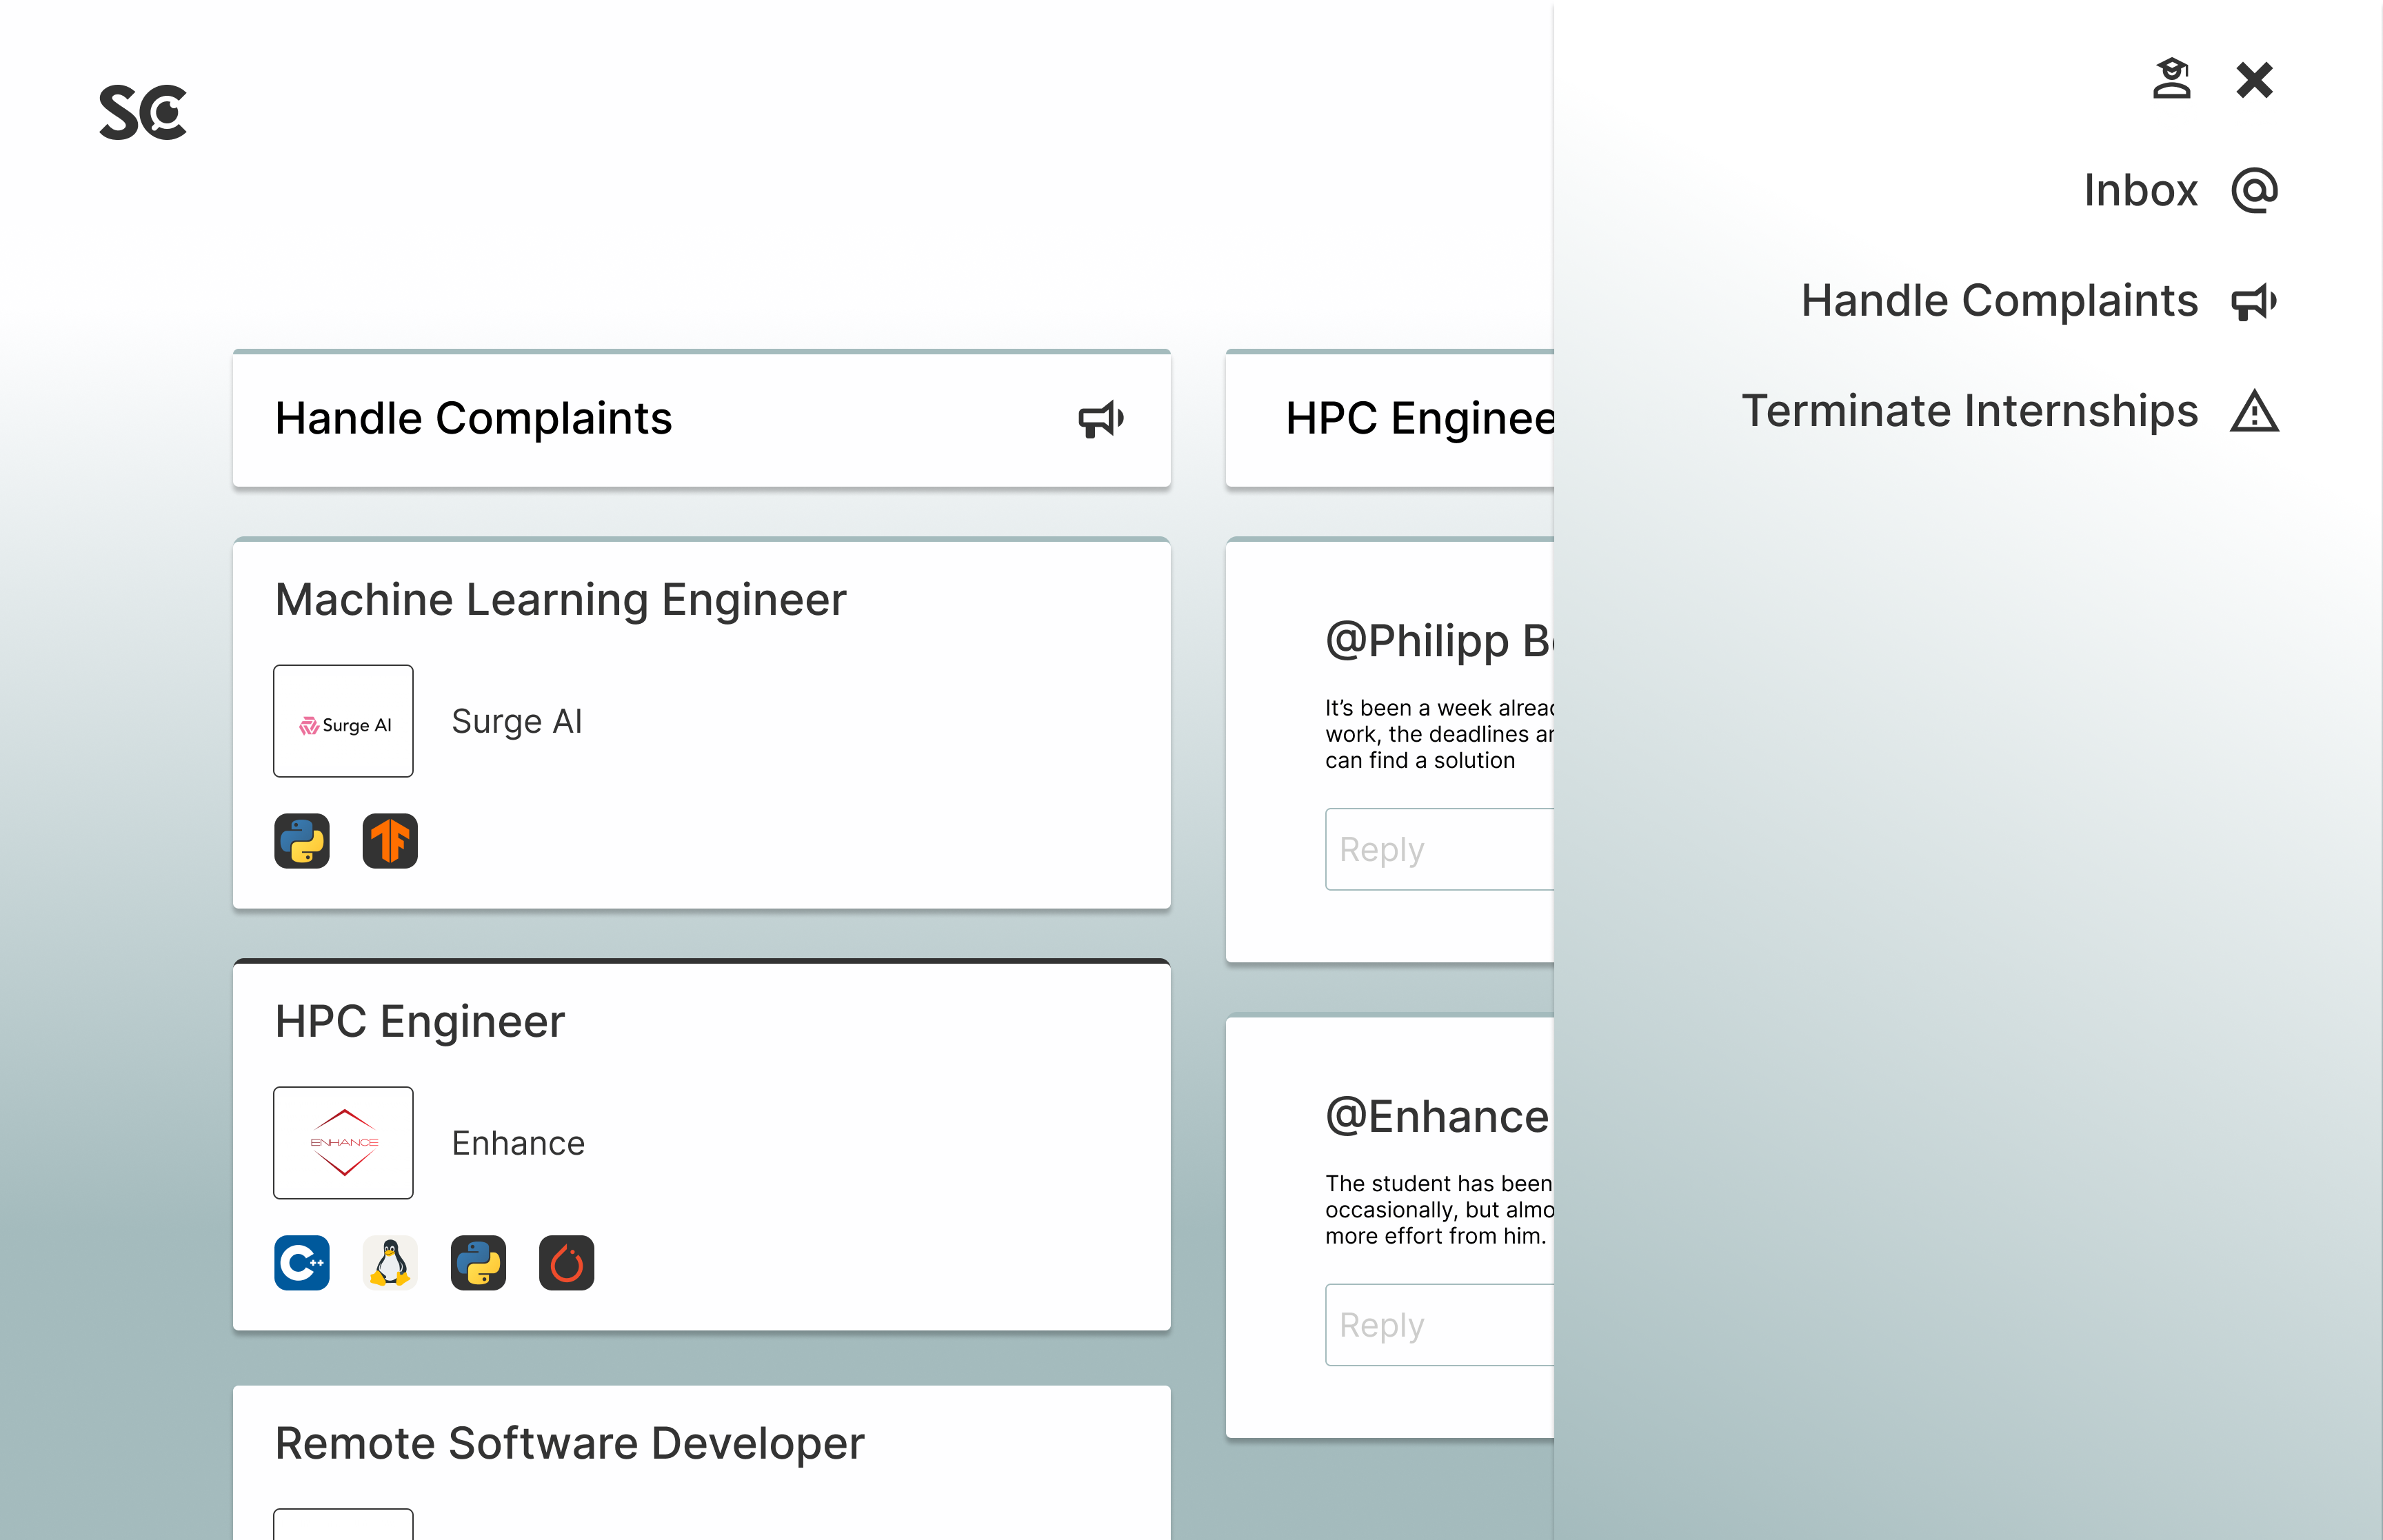
\includegraphics[width=0.8\textwidth]{Images/ui/Sidebar Uni}
%    \caption{University Menu}
%    \label{fig:menuUni}
%\end{figure}